\documentclass[
	a4paper,
	titlepage,
	twoside,
	headinclude=true,
	footinclude=false,
	openright,
	pdfspacing,
	10pt,
	numbers=noenddot,
	manychapters,
	draft
%	final
]{scrbook} %BCOR=5mm
\usepackage[T1]{fontenc}
\usepackage[utf8]{inputenc}
\usepackage[english,italian]{babel}

\usepackage[
	table,
	dvipsnames,
	usenames
]{xcolor}
%\definecolor{halfgray}{gray}{0.55} % chapter numbers will be semi transparent .5 .55 .6 .0
\definecolor{webgreen}{rgb}{0,.5,0}
\definecolor{webbrown}{rgb}{.6,0,0}
\definecolor{Maroon}{cmyk}{0, 0.87, 0.68, 0.32}
\definecolor{RoyalBlue}{cmyk}{1, 0.50, 0, 0}
\definecolor{mygreen}{rgb}{0,0.5,0}

\usepackage[italian]{varioref}

%% ****************************************************************************************************
% classicthesis-config.tex 
% formerly known as loadpackages.sty, classicthesis-ldpkg.sty, and classicthesis-preamble.sty 
% Use it at the beginning of your ClassicThesis.tex, or as a LaTeX Preamble 
% in your ClassicThesis.{tex,lyx} with % ****************************************************************************************************
% classicthesis-config.tex 
% formerly known as loadpackages.sty, classicthesis-ldpkg.sty, and classicthesis-preamble.sty 
% Use it at the beginning of your ClassicThesis.tex, or as a LaTeX Preamble 
% in your ClassicThesis.{tex,lyx} with % ****************************************************************************************************
% classicthesis-config.tex 
% formerly known as loadpackages.sty, classicthesis-ldpkg.sty, and classicthesis-preamble.sty 
% Use it at the beginning of your ClassicThesis.tex, or as a LaTeX Preamble 
% in your ClassicThesis.{tex,lyx} with \input{classicthesis-config}
% ****************************************************************************************************  
% If you like the classicthesis, then I would appreciate a postcard. 
% My address can be found in the file ClassicThesis.pdf. A collection 
% of the postcards I received so far is available online at 
% http://postcards.miede.de
% ****************************************************************************************************

% ****************************************************************************************************
% 1. Configure classicthesis for your needs here, e.g., remove "drafting" below 
% in order to deactivate the time-stamp on the pages
% ****************************************************************************************************
\PassOptionsToPackage{eulerchapternumbers,listings,drafting,%
				 pdfspacing,floatperchapter,%linedheaders,%
				 subfig,beramono,eulermath,parts}{classicthesis}										
% ********************************************************************
% Available options for classicthesis.sty 
% (see ClassicThesis.pdf for more information):
% drafting
% parts nochapters linedheaders
% eulerchapternumbers beramono eulermath pdfspacing minionprospacing
% tocaligned dottedtoc manychapters
% listings floatperchapter subfig
% ********************************************************************

% ********************************************************************
% Triggers for this config
% ******************************************************************** 
\usepackage{ifthen}
\newboolean{enable-backrefs} % enable backrefs in the bibliography
\setboolean{enable-backrefs}{false} % true false
% ****************************************************************************************************


% ****************************************************************************************************
% 2. Personal data and user ad-hoc commands
% ****************************************************************************************************
\newcommand{\myTitle}{Appunti di Laboratorio d'Informatica}
\newcommand{\mySubtitle}{}
\newcommand{\myDegree}{}
\newcommand{\myName}{Paolo Di Giglio}
\newcommand{\myProf}{Bernardinello, Luca}
\newcommand{\myOtherProf}{}
\newcommand{\mySupervisor}{}
\newcommand{\myFaculty}{Fisica}
\newcommand{\myDepartment}{G. Occhialini}
\newcommand{\myUni}{Università degli Studi di Milano Bicocca}
\newcommand{\myLocation}{}
\newcommand{\myTime}{\today}
\newcommand{\myVersion}{}

% ********************************************************************
% Setup, finetuning, and useful commands
% ********************************************************************
\newcounter{dummy} % necessary for correct hyperlinks (to index, bib, etc.)
\newlength{\abcd} % for ab..z string length calculation
\providecommand{\mLyX}{L\kern-.1667em\lower.25em\hbox{Y}\kern-.125emX\@}
\newcommand{\ie}{i.\,e.}
\newcommand{\Ie}{I.\,e.}
\newcommand{\eg}{e.\,g.}
\newcommand{\Eg}{E.\,g.} 
% ****************************************************************************************************


% ****************************************************************************************************
% 3. Loading some handy packages
% ****************************************************************************************************
% ******************************************************************** 
% Packages with options that might require adjustments
% ******************************************************************** 
\PassOptionsToPackage{latin9}{inputenc}	% latin9 (ISO-8859-9) = latin1+"Euro sign"
 \usepackage{inputenc}				

%\PassOptionsToPackage{ngerman,american}{babel}   % change this to your language(s)
% Spanish languages need extra options in order to work with this template
%\PassOptionsToPackage{spanish,es-lcroman}{babel}
 \usepackage{babel}					

\PassOptionsToPackage{square,numbers}{natbib}
 \usepackage{natbib}				

\PassOptionsToPackage{fleqn}{amsmath}		% math environments and more by the AMS 
 \usepackage{amsmath}

% ******************************************************************** 
% General useful packages
% ******************************************************************** 
\PassOptionsToPackage{T1}{fontenc} % T2A for cyrillics
	\usepackage{fontenc}                 
\usepackage{xspace} % to get the spacing after macros right  
\usepackage{mparhack} % get marginpar right
\usepackage{fixltx2e} % fixes some LaTeX stuff 
\PassOptionsToPackage{printonlyused,smaller}{acronym}
	\usepackage{acronym} % nice macros for handling all acronyms in the thesis
%\renewcommand*{\acsfont}[1]{\textssc{#1}} % for MinionPro
\renewcommand{\bflabel}[1]{{#1}\hfill} % fix the list of acronyms
% ****************************************************************************************************


% ****************************************************************************************************
% 4. Setup floats: tables, (sub)figures, and captions
% ****************************************************************************************************
\usepackage{tabularx} % better tables
	\setlength{\extrarowheight}{3pt} % increase table row height
\newcommand{\tableheadline}[1]{\multicolumn{1}{c}{\spacedlowsmallcaps{#1}}}
\newcommand{\myfloatalign}{\centering} % to be used with each float for alignment
\usepackage{caption}
\captionsetup{format=hang,font=small}
\usepackage{subfig}  
% ****************************************************************************************************


% ****************************************************************************************************
% 5. Setup code listings
% ****************************************************************************************************
\PassOptionsToPackage{final}{listings}
	\usepackage{listings}

\lstset{language=[Ansi]C,%[LaTeX]Tex,%C++,
    keywordstyle=\color{RoyalBlue},%\bfseries,
    basicstyle=\small\ttfamily,
    %identifierstyle=\color{NavyBlue},
    commentstyle=\itshape\color{Green}\ttfamily,
    stringstyle=\color{PineGreen},%\color{darkgray},
    numbers=left,% none
    numberstyle=\scriptsize,%\tiny
    stepnumber=2,
    numbersep=8pt,
    showstringspaces=false,
    breaklines=true,
    frameround=ftff,
 %   frame=single,
    belowcaptionskip=.75\baselineskip,
    tabsize=4,
    frame=L,
    escapeinside={£!}{!£}
} 

% in italiano
\addto\captionsitalian{\renewcommand{\lstlistingname}{Codice}}
\addto\captionsitalian{\renewcommand{\lstlistlistingname}{Elenco dei codici}}
% ****************************************************************************************************    		   


% ****************************************************************************************************
% 6. PDFLaTeX, hyperreferences and citation backreferences
% ****************************************************************************************************
% ********************************************************************
% Using PDFLaTeX
% ********************************************************************
\PassOptionsToPackage{pdftex,hyperfootnotes=true,pdfpagelabels}{hyperref}
	\usepackage{hyperref}  % backref linktocpage pagebackref
\pdfcompresslevel=9
\pdfadjustspacing=1 
\PassOptionsToPackage{pdftex}{graphicx}
	\usepackage{graphicx} 

% ********************************************************************
% Setup the style of the backrefs from the bibliography
% (translate the options to any language you use)
% ********************************************************************
\newcommand{\backrefnotcitedstring}{\relax}%(Not cited.)
\newcommand{\backrefcitedsinglestring}[1]{(Cited on page~#1.)}
\newcommand{\backrefcitedmultistring}[1]{(Cited on pages~#1.)}
\ifthenelse{\boolean{enable-backrefs}}%
{%
		\PassOptionsToPackage{hyperpageref}{backref}
		\usepackage{backref} % to be loaded after hyperref package 
		   \renewcommand{\backreftwosep}{ and~} % separate 2 pages
		   \renewcommand{\backreflastsep}{, and~} % separate last of longer list
		   \renewcommand*{\backref}[1]{}  % disable standard
		   \renewcommand*{\backrefalt}[4]{% detailed backref
		      \ifcase #1 %
		         \backrefnotcitedstring%
		      \or%
		         \backrefcitedsinglestring{#2}%
		      \else%
		         \backrefcitedmultistring{#2}%
		      \fi}%
}{\relax}    

% ********************************************************************
% Hyperreferences
% ********************************************************************
\hypersetup{%
    %draft,	% = no hyperlinking at all (useful in b/w printouts)
    colorlinks=true, linktocpage=true, pdfstartpage=3, pdfstartview=FitV,%
    % uncomment the following line if you want to have black links (e.g., for printing)
    %colorlinks=false, linktocpage=false, pdfborder={0 0 0}, pdfstartpage=3, pdfstartview=FitV,% 
    breaklinks=true, pdfpagemode=UseNone, pageanchor=true, pdfpagemode=UseOutlines,%
    plainpages=false, bookmarksnumbered, bookmarksopen=true, bookmarksopenlevel=1,%
    hypertexnames=true, pdfhighlight=/O,%nesting=true,%frenchlinks,%
    urlcolor=webbrown, linkcolor=RoyalBlue, citecolor=webgreen, %pagecolor=RoyalBlue,%
    %urlcolor=Black, linkcolor=Black, citecolor=Black, %pagecolor=Black,%
    pdftitle={\myTitle},%
    pdfauthor={\textcopyright\ \myName, \myUni, \myFaculty},%
    pdfsubject={},%
    pdfkeywords={},%
    pdfcreator={pdfLaTeX},%
    pdfproducer={LaTeX with hyperref and classicthesis}%
}   

% ********************************************************************
% Setup autoreferences
% ********************************************************************
% There are some issues regarding autorefnames
% http://www.ureader.de/msg/136221647.aspx
% http://www.tex.ac.uk/cgi-bin/texfaq2html?label=latexwords
% you have to redefine the makros for the 
% language you use, e.g., american, ngerman
% (as chosen when loading babel/AtBeginDocument)
% ********************************************************************
\makeatletter
\@ifpackageloaded{babel}%
    {%
       \addto\extrasamerican{%
					\renewcommand*{\figureautorefname}{Figure}%
					\renewcommand*{\tableautorefname}{Table}%
					\renewcommand*{\partautorefname}{Part}%
					\renewcommand*{\chapterautorefname}{Chapter}%
					\renewcommand*{\sectionautorefname}{Section}%
					\renewcommand*{\subsectionautorefname}{Section}%
					\renewcommand*{\subsubsectionautorefname}{Section}% 	
				}%
       \addto\extrasngerman{% 
					\renewcommand*{\paragraphautorefname}{Absatz}%
					\renewcommand*{\subparagraphautorefname}{Unterabsatz}%
					\renewcommand*{\footnoteautorefname}{Fu\"snote}%
					\renewcommand*{\FancyVerbLineautorefname}{Zeile}%
					\renewcommand*{\theoremautorefname}{Theorem}%
					\renewcommand*{\appendixautorefname}{Anhang}%
					\renewcommand*{\equationautorefname}{Gleichung}%        
					\renewcommand*{\itemautorefname}{Punkt}%
				}%	
			% Fix to getting autorefs for subfigures right (thanks to Belinda Vogt for changing the definition)
			\providecommand{\subfigureautorefname}{\figureautorefname}%  			
    }{\relax}
\makeatother


% ****************************************************************************************************
% 7. Last calls before the bar closes
% ****************************************************************************************************
% ********************************************************************
% Development Stuff
% ********************************************************************
\listfiles
%\PassOptionsToPackage{l2tabu,orthodox,abort}{nag}
%	\usepackage{nag}
%\PassOptionsToPackage{warning, all}{onlyamsmath}
%	\usepackage{onlyamsmath}

% ********************************************************************
% Last, but not least...
% ********************************************************************
\usepackage{classicthesis} 
% ****************************************************************************************************


% ****************************************************************************************************
% 8. Further adjustments (experimental)
% ****************************************************************************************************
% ********************************************************************
% Changing the text area
% ********************************************************************
%\linespread{1.05} % a bit more for Palatino
%\areaset[current]{312pt}{761pt} % 686 (factor 2.2) + 33 head + 42 head \the\footskip
%\setlength{\marginparwidth}{7em}%
%\setlength{\marginparsep}{2em}%

% ********************************************************************
% Using different fonts
% ********************************************************************
%\usepackage[oldstylenums]{kpfonts} % oldstyle notextcomp
%\usepackage[osf]{libertine}
%\usepackage{hfoldsty} % Computer Modern with osf
%\usepackage[light,condensed,math]{iwona}
%\renewcommand{\sfdefault}{iwona}
%\usepackage{lmodern} % <-- no osf support :-(
%\usepackage[urw-garamond]{mathdesign} <-- no osf support :-(
% ****************************************************************************************************

% ****************************************************************************************************  
% If you like the classicthesis, then I would appreciate a postcard. 
% My address can be found in the file ClassicThesis.pdf. A collection 
% of the postcards I received so far is available online at 
% http://postcards.miede.de
% ****************************************************************************************************

% ****************************************************************************************************
% 1. Configure classicthesis for your needs here, e.g., remove "drafting" below 
% in order to deactivate the time-stamp on the pages
% ****************************************************************************************************
\PassOptionsToPackage{eulerchapternumbers,listings,drafting,%
				 pdfspacing,floatperchapter,%linedheaders,%
				 subfig,beramono,eulermath,parts}{classicthesis}										
% ********************************************************************
% Available options for classicthesis.sty 
% (see ClassicThesis.pdf for more information):
% drafting
% parts nochapters linedheaders
% eulerchapternumbers beramono eulermath pdfspacing minionprospacing
% tocaligned dottedtoc manychapters
% listings floatperchapter subfig
% ********************************************************************

% ********************************************************************
% Triggers for this config
% ******************************************************************** 
\usepackage{ifthen}
\newboolean{enable-backrefs} % enable backrefs in the bibliography
\setboolean{enable-backrefs}{false} % true false
% ****************************************************************************************************


% ****************************************************************************************************
% 2. Personal data and user ad-hoc commands
% ****************************************************************************************************
\newcommand{\myTitle}{Appunti di Laboratorio d'Informatica}
\newcommand{\mySubtitle}{}
\newcommand{\myDegree}{}
\newcommand{\myName}{Paolo Di Giglio}
\newcommand{\myProf}{Bernardinello, Luca}
\newcommand{\myOtherProf}{}
\newcommand{\mySupervisor}{}
\newcommand{\myFaculty}{Fisica}
\newcommand{\myDepartment}{G. Occhialini}
\newcommand{\myUni}{Università degli Studi di Milano Bicocca}
\newcommand{\myLocation}{}
\newcommand{\myTime}{\today}
\newcommand{\myVersion}{}

% ********************************************************************
% Setup, finetuning, and useful commands
% ********************************************************************
\newcounter{dummy} % necessary for correct hyperlinks (to index, bib, etc.)
\newlength{\abcd} % for ab..z string length calculation
\providecommand{\mLyX}{L\kern-.1667em\lower.25em\hbox{Y}\kern-.125emX\@}
\newcommand{\ie}{i.\,e.}
\newcommand{\Ie}{I.\,e.}
\newcommand{\eg}{e.\,g.}
\newcommand{\Eg}{E.\,g.} 
% ****************************************************************************************************


% ****************************************************************************************************
% 3. Loading some handy packages
% ****************************************************************************************************
% ******************************************************************** 
% Packages with options that might require adjustments
% ******************************************************************** 
\PassOptionsToPackage{latin9}{inputenc}	% latin9 (ISO-8859-9) = latin1+"Euro sign"
 \usepackage{inputenc}				

%\PassOptionsToPackage{ngerman,american}{babel}   % change this to your language(s)
% Spanish languages need extra options in order to work with this template
%\PassOptionsToPackage{spanish,es-lcroman}{babel}
 \usepackage{babel}					

\PassOptionsToPackage{square,numbers}{natbib}
 \usepackage{natbib}				

\PassOptionsToPackage{fleqn}{amsmath}		% math environments and more by the AMS 
 \usepackage{amsmath}

% ******************************************************************** 
% General useful packages
% ******************************************************************** 
\PassOptionsToPackage{T1}{fontenc} % T2A for cyrillics
	\usepackage{fontenc}                 
\usepackage{xspace} % to get the spacing after macros right  
\usepackage{mparhack} % get marginpar right
\usepackage{fixltx2e} % fixes some LaTeX stuff 
\PassOptionsToPackage{printonlyused,smaller}{acronym}
	\usepackage{acronym} % nice macros for handling all acronyms in the thesis
%\renewcommand*{\acsfont}[1]{\textssc{#1}} % for MinionPro
\renewcommand{\bflabel}[1]{{#1}\hfill} % fix the list of acronyms
% ****************************************************************************************************


% ****************************************************************************************************
% 4. Setup floats: tables, (sub)figures, and captions
% ****************************************************************************************************
\usepackage{tabularx} % better tables
	\setlength{\extrarowheight}{3pt} % increase table row height
\newcommand{\tableheadline}[1]{\multicolumn{1}{c}{\spacedlowsmallcaps{#1}}}
\newcommand{\myfloatalign}{\centering} % to be used with each float for alignment
\usepackage{caption}
\captionsetup{format=hang,font=small}
\usepackage{subfig}  
% ****************************************************************************************************


% ****************************************************************************************************
% 5. Setup code listings
% ****************************************************************************************************
\PassOptionsToPackage{final}{listings}
	\usepackage{listings}

\lstset{language=[Ansi]C,%[LaTeX]Tex,%C++,
    keywordstyle=\color{RoyalBlue},%\bfseries,
    basicstyle=\small\ttfamily,
    %identifierstyle=\color{NavyBlue},
    commentstyle=\itshape\color{Green}\ttfamily,
    stringstyle=\color{PineGreen},%\color{darkgray},
    numbers=left,% none
    numberstyle=\scriptsize,%\tiny
    stepnumber=2,
    numbersep=8pt,
    showstringspaces=false,
    breaklines=true,
    frameround=ftff,
 %   frame=single,
    belowcaptionskip=.75\baselineskip,
    tabsize=4,
    frame=L,
    escapeinside={£!}{!£}
} 

% in italiano
\addto\captionsitalian{\renewcommand{\lstlistingname}{Codice}}
\addto\captionsitalian{\renewcommand{\lstlistlistingname}{Elenco dei codici}}
% ****************************************************************************************************    		   


% ****************************************************************************************************
% 6. PDFLaTeX, hyperreferences and citation backreferences
% ****************************************************************************************************
% ********************************************************************
% Using PDFLaTeX
% ********************************************************************
\PassOptionsToPackage{pdftex,hyperfootnotes=true,pdfpagelabels}{hyperref}
	\usepackage{hyperref}  % backref linktocpage pagebackref
\pdfcompresslevel=9
\pdfadjustspacing=1 
\PassOptionsToPackage{pdftex}{graphicx}
	\usepackage{graphicx} 

% ********************************************************************
% Setup the style of the backrefs from the bibliography
% (translate the options to any language you use)
% ********************************************************************
\newcommand{\backrefnotcitedstring}{\relax}%(Not cited.)
\newcommand{\backrefcitedsinglestring}[1]{(Cited on page~#1.)}
\newcommand{\backrefcitedmultistring}[1]{(Cited on pages~#1.)}
\ifthenelse{\boolean{enable-backrefs}}%
{%
		\PassOptionsToPackage{hyperpageref}{backref}
		\usepackage{backref} % to be loaded after hyperref package 
		   \renewcommand{\backreftwosep}{ and~} % separate 2 pages
		   \renewcommand{\backreflastsep}{, and~} % separate last of longer list
		   \renewcommand*{\backref}[1]{}  % disable standard
		   \renewcommand*{\backrefalt}[4]{% detailed backref
		      \ifcase #1 %
		         \backrefnotcitedstring%
		      \or%
		         \backrefcitedsinglestring{#2}%
		      \else%
		         \backrefcitedmultistring{#2}%
		      \fi}%
}{\relax}    

% ********************************************************************
% Hyperreferences
% ********************************************************************
\hypersetup{%
    %draft,	% = no hyperlinking at all (useful in b/w printouts)
    colorlinks=true, linktocpage=true, pdfstartpage=3, pdfstartview=FitV,%
    % uncomment the following line if you want to have black links (e.g., for printing)
    %colorlinks=false, linktocpage=false, pdfborder={0 0 0}, pdfstartpage=3, pdfstartview=FitV,% 
    breaklinks=true, pdfpagemode=UseNone, pageanchor=true, pdfpagemode=UseOutlines,%
    plainpages=false, bookmarksnumbered, bookmarksopen=true, bookmarksopenlevel=1,%
    hypertexnames=true, pdfhighlight=/O,%nesting=true,%frenchlinks,%
    urlcolor=webbrown, linkcolor=RoyalBlue, citecolor=webgreen, %pagecolor=RoyalBlue,%
    %urlcolor=Black, linkcolor=Black, citecolor=Black, %pagecolor=Black,%
    pdftitle={\myTitle},%
    pdfauthor={\textcopyright\ \myName, \myUni, \myFaculty},%
    pdfsubject={},%
    pdfkeywords={},%
    pdfcreator={pdfLaTeX},%
    pdfproducer={LaTeX with hyperref and classicthesis}%
}   

% ********************************************************************
% Setup autoreferences
% ********************************************************************
% There are some issues regarding autorefnames
% http://www.ureader.de/msg/136221647.aspx
% http://www.tex.ac.uk/cgi-bin/texfaq2html?label=latexwords
% you have to redefine the makros for the 
% language you use, e.g., american, ngerman
% (as chosen when loading babel/AtBeginDocument)
% ********************************************************************
\makeatletter
\@ifpackageloaded{babel}%
    {%
       \addto\extrasamerican{%
					\renewcommand*{\figureautorefname}{Figure}%
					\renewcommand*{\tableautorefname}{Table}%
					\renewcommand*{\partautorefname}{Part}%
					\renewcommand*{\chapterautorefname}{Chapter}%
					\renewcommand*{\sectionautorefname}{Section}%
					\renewcommand*{\subsectionautorefname}{Section}%
					\renewcommand*{\subsubsectionautorefname}{Section}% 	
				}%
       \addto\extrasngerman{% 
					\renewcommand*{\paragraphautorefname}{Absatz}%
					\renewcommand*{\subparagraphautorefname}{Unterabsatz}%
					\renewcommand*{\footnoteautorefname}{Fu\"snote}%
					\renewcommand*{\FancyVerbLineautorefname}{Zeile}%
					\renewcommand*{\theoremautorefname}{Theorem}%
					\renewcommand*{\appendixautorefname}{Anhang}%
					\renewcommand*{\equationautorefname}{Gleichung}%        
					\renewcommand*{\itemautorefname}{Punkt}%
				}%	
			% Fix to getting autorefs for subfigures right (thanks to Belinda Vogt for changing the definition)
			\providecommand{\subfigureautorefname}{\figureautorefname}%  			
    }{\relax}
\makeatother


% ****************************************************************************************************
% 7. Last calls before the bar closes
% ****************************************************************************************************
% ********************************************************************
% Development Stuff
% ********************************************************************
\listfiles
%\PassOptionsToPackage{l2tabu,orthodox,abort}{nag}
%	\usepackage{nag}
%\PassOptionsToPackage{warning, all}{onlyamsmath}
%	\usepackage{onlyamsmath}

% ********************************************************************
% Last, but not least...
% ********************************************************************
\usepackage{classicthesis} 
% ****************************************************************************************************


% ****************************************************************************************************
% 8. Further adjustments (experimental)
% ****************************************************************************************************
% ********************************************************************
% Changing the text area
% ********************************************************************
%\linespread{1.05} % a bit more for Palatino
%\areaset[current]{312pt}{761pt} % 686 (factor 2.2) + 33 head + 42 head \the\footskip
%\setlength{\marginparwidth}{7em}%
%\setlength{\marginparsep}{2em}%

% ********************************************************************
% Using different fonts
% ********************************************************************
%\usepackage[oldstylenums]{kpfonts} % oldstyle notextcomp
%\usepackage[osf]{libertine}
%\usepackage{hfoldsty} % Computer Modern with osf
%\usepackage[light,condensed,math]{iwona}
%\renewcommand{\sfdefault}{iwona}
%\usepackage{lmodern} % <-- no osf support :-(
%\usepackage[urw-garamond]{mathdesign} <-- no osf support :-(
% ****************************************************************************************************

% ****************************************************************************************************  
% If you like the classicthesis, then I would appreciate a postcard. 
% My address can be found in the file ClassicThesis.pdf. A collection 
% of the postcards I received so far is available online at 
% http://postcards.miede.de
% ****************************************************************************************************

% ****************************************************************************************************
% 1. Configure classicthesis for your needs here, e.g., remove "drafting" below 
% in order to deactivate the time-stamp on the pages
% ****************************************************************************************************
\PassOptionsToPackage{eulerchapternumbers,listings,drafting,%
				 pdfspacing,floatperchapter,%linedheaders,%
				 subfig,beramono,eulermath,parts}{classicthesis}										
% ********************************************************************
% Available options for classicthesis.sty 
% (see ClassicThesis.pdf for more information):
% drafting
% parts nochapters linedheaders
% eulerchapternumbers beramono eulermath pdfspacing minionprospacing
% tocaligned dottedtoc manychapters
% listings floatperchapter subfig
% ********************************************************************

% ********************************************************************
% Triggers for this config
% ******************************************************************** 
\usepackage{ifthen}
\newboolean{enable-backrefs} % enable backrefs in the bibliography
\setboolean{enable-backrefs}{false} % true false
% ****************************************************************************************************


% ****************************************************************************************************
% 2. Personal data and user ad-hoc commands
% ****************************************************************************************************
\newcommand{\myTitle}{Appunti di Laboratorio d'Informatica}
\newcommand{\mySubtitle}{}
\newcommand{\myDegree}{}
\newcommand{\myName}{Paolo Di Giglio}
\newcommand{\myProf}{Bernardinello, Luca}
\newcommand{\myOtherProf}{}
\newcommand{\mySupervisor}{}
\newcommand{\myFaculty}{Fisica}
\newcommand{\myDepartment}{G. Occhialini}
\newcommand{\myUni}{Università degli Studi di Milano Bicocca}
\newcommand{\myLocation}{}
\newcommand{\myTime}{\today}
\newcommand{\myVersion}{}

% ********************************************************************
% Setup, finetuning, and useful commands
% ********************************************************************
\newcounter{dummy} % necessary for correct hyperlinks (to index, bib, etc.)
\newlength{\abcd} % for ab..z string length calculation
\providecommand{\mLyX}{L\kern-.1667em\lower.25em\hbox{Y}\kern-.125emX\@}
\newcommand{\ie}{i.\,e.}
\newcommand{\Ie}{I.\,e.}
\newcommand{\eg}{e.\,g.}
\newcommand{\Eg}{E.\,g.} 
% ****************************************************************************************************


% ****************************************************************************************************
% 3. Loading some handy packages
% ****************************************************************************************************
% ******************************************************************** 
% Packages with options that might require adjustments
% ******************************************************************** 
\PassOptionsToPackage{latin9}{inputenc}	% latin9 (ISO-8859-9) = latin1+"Euro sign"
 \usepackage{inputenc}				

%\PassOptionsToPackage{ngerman,american}{babel}   % change this to your language(s)
% Spanish languages need extra options in order to work with this template
%\PassOptionsToPackage{spanish,es-lcroman}{babel}
 \usepackage{babel}					

\PassOptionsToPackage{square,numbers}{natbib}
 \usepackage{natbib}				

\PassOptionsToPackage{fleqn}{amsmath}		% math environments and more by the AMS 
 \usepackage{amsmath}

% ******************************************************************** 
% General useful packages
% ******************************************************************** 
\PassOptionsToPackage{T1}{fontenc} % T2A for cyrillics
	\usepackage{fontenc}                 
\usepackage{xspace} % to get the spacing after macros right  
\usepackage{mparhack} % get marginpar right
\usepackage{fixltx2e} % fixes some LaTeX stuff 
\PassOptionsToPackage{printonlyused,smaller}{acronym}
	\usepackage{acronym} % nice macros for handling all acronyms in the thesis
%\renewcommand*{\acsfont}[1]{\textssc{#1}} % for MinionPro
\renewcommand{\bflabel}[1]{{#1}\hfill} % fix the list of acronyms
% ****************************************************************************************************


% ****************************************************************************************************
% 4. Setup floats: tables, (sub)figures, and captions
% ****************************************************************************************************
\usepackage{tabularx} % better tables
	\setlength{\extrarowheight}{3pt} % increase table row height
\newcommand{\tableheadline}[1]{\multicolumn{1}{c}{\spacedlowsmallcaps{#1}}}
\newcommand{\myfloatalign}{\centering} % to be used with each float for alignment
\usepackage{caption}
\captionsetup{format=hang,font=small}
\usepackage{subfig}  
% ****************************************************************************************************


% ****************************************************************************************************
% 5. Setup code listings
% ****************************************************************************************************
\PassOptionsToPackage{final}{listings}
	\usepackage{listings}

\lstset{language=[Ansi]C,%[LaTeX]Tex,%C++,
    keywordstyle=\color{RoyalBlue},%\bfseries,
    basicstyle=\small\ttfamily,
    %identifierstyle=\color{NavyBlue},
    commentstyle=\itshape\color{Green}\ttfamily,
    stringstyle=\color{PineGreen},%\color{darkgray},
    numbers=left,% none
    numberstyle=\scriptsize,%\tiny
    stepnumber=2,
    numbersep=8pt,
    showstringspaces=false,
    breaklines=true,
    frameround=ftff,
 %   frame=single,
    belowcaptionskip=.75\baselineskip,
    tabsize=4,
    frame=L,
    escapeinside={£!}{!£}
} 

% in italiano
\addto\captionsitalian{\renewcommand{\lstlistingname}{Codice}}
\addto\captionsitalian{\renewcommand{\lstlistlistingname}{Elenco dei codici}}
% ****************************************************************************************************    		   


% ****************************************************************************************************
% 6. PDFLaTeX, hyperreferences and citation backreferences
% ****************************************************************************************************
% ********************************************************************
% Using PDFLaTeX
% ********************************************************************
\PassOptionsToPackage{pdftex,hyperfootnotes=true,pdfpagelabels}{hyperref}
	\usepackage{hyperref}  % backref linktocpage pagebackref
\pdfcompresslevel=9
\pdfadjustspacing=1 
\PassOptionsToPackage{pdftex}{graphicx}
	\usepackage{graphicx} 

% ********************************************************************
% Setup the style of the backrefs from the bibliography
% (translate the options to any language you use)
% ********************************************************************
\newcommand{\backrefnotcitedstring}{\relax}%(Not cited.)
\newcommand{\backrefcitedsinglestring}[1]{(Cited on page~#1.)}
\newcommand{\backrefcitedmultistring}[1]{(Cited on pages~#1.)}
\ifthenelse{\boolean{enable-backrefs}}%
{%
		\PassOptionsToPackage{hyperpageref}{backref}
		\usepackage{backref} % to be loaded after hyperref package 
		   \renewcommand{\backreftwosep}{ and~} % separate 2 pages
		   \renewcommand{\backreflastsep}{, and~} % separate last of longer list
		   \renewcommand*{\backref}[1]{}  % disable standard
		   \renewcommand*{\backrefalt}[4]{% detailed backref
		      \ifcase #1 %
		         \backrefnotcitedstring%
		      \or%
		         \backrefcitedsinglestring{#2}%
		      \else%
		         \backrefcitedmultistring{#2}%
		      \fi}%
}{\relax}    

% ********************************************************************
% Hyperreferences
% ********************************************************************
\hypersetup{%
    %draft,	% = no hyperlinking at all (useful in b/w printouts)
    colorlinks=true, linktocpage=true, pdfstartpage=3, pdfstartview=FitV,%
    % uncomment the following line if you want to have black links (e.g., for printing)
    %colorlinks=false, linktocpage=false, pdfborder={0 0 0}, pdfstartpage=3, pdfstartview=FitV,% 
    breaklinks=true, pdfpagemode=UseNone, pageanchor=true, pdfpagemode=UseOutlines,%
    plainpages=false, bookmarksnumbered, bookmarksopen=true, bookmarksopenlevel=1,%
    hypertexnames=true, pdfhighlight=/O,%nesting=true,%frenchlinks,%
    urlcolor=webbrown, linkcolor=RoyalBlue, citecolor=webgreen, %pagecolor=RoyalBlue,%
    %urlcolor=Black, linkcolor=Black, citecolor=Black, %pagecolor=Black,%
    pdftitle={\myTitle},%
    pdfauthor={\textcopyright\ \myName, \myUni, \myFaculty},%
    pdfsubject={},%
    pdfkeywords={},%
    pdfcreator={pdfLaTeX},%
    pdfproducer={LaTeX with hyperref and classicthesis}%
}   

% ********************************************************************
% Setup autoreferences
% ********************************************************************
% There are some issues regarding autorefnames
% http://www.ureader.de/msg/136221647.aspx
% http://www.tex.ac.uk/cgi-bin/texfaq2html?label=latexwords
% you have to redefine the makros for the 
% language you use, e.g., american, ngerman
% (as chosen when loading babel/AtBeginDocument)
% ********************************************************************
\makeatletter
\@ifpackageloaded{babel}%
    {%
       \addto\extrasamerican{%
					\renewcommand*{\figureautorefname}{Figure}%
					\renewcommand*{\tableautorefname}{Table}%
					\renewcommand*{\partautorefname}{Part}%
					\renewcommand*{\chapterautorefname}{Chapter}%
					\renewcommand*{\sectionautorefname}{Section}%
					\renewcommand*{\subsectionautorefname}{Section}%
					\renewcommand*{\subsubsectionautorefname}{Section}% 	
				}%
       \addto\extrasngerman{% 
					\renewcommand*{\paragraphautorefname}{Absatz}%
					\renewcommand*{\subparagraphautorefname}{Unterabsatz}%
					\renewcommand*{\footnoteautorefname}{Fu\"snote}%
					\renewcommand*{\FancyVerbLineautorefname}{Zeile}%
					\renewcommand*{\theoremautorefname}{Theorem}%
					\renewcommand*{\appendixautorefname}{Anhang}%
					\renewcommand*{\equationautorefname}{Gleichung}%        
					\renewcommand*{\itemautorefname}{Punkt}%
				}%	
			% Fix to getting autorefs for subfigures right (thanks to Belinda Vogt for changing the definition)
			\providecommand{\subfigureautorefname}{\figureautorefname}%  			
    }{\relax}
\makeatother


% ****************************************************************************************************
% 7. Last calls before the bar closes
% ****************************************************************************************************
% ********************************************************************
% Development Stuff
% ********************************************************************
\listfiles
%\PassOptionsToPackage{l2tabu,orthodox,abort}{nag}
%	\usepackage{nag}
%\PassOptionsToPackage{warning, all}{onlyamsmath}
%	\usepackage{onlyamsmath}

% ********************************************************************
% Last, but not least...
% ********************************************************************
\usepackage{classicthesis} 
% ****************************************************************************************************


% ****************************************************************************************************
% 8. Further adjustments (experimental)
% ****************************************************************************************************
% ********************************************************************
% Changing the text area
% ********************************************************************
%\linespread{1.05} % a bit more for Palatino
%\areaset[current]{312pt}{761pt} % 686 (factor 2.2) + 33 head + 42 head \the\footskip
%\setlength{\marginparwidth}{7em}%
%\setlength{\marginparsep}{2em}%

% ********************************************************************
% Using different fonts
% ********************************************************************
%\usepackage[oldstylenums]{kpfonts} % oldstyle notextcomp
%\usepackage[osf]{libertine}
%\usepackage{hfoldsty} % Computer Modern with osf
%\usepackage[light,condensed,math]{iwona}
%\renewcommand{\sfdefault}{iwona}
%\usepackage{lmodern} % <-- no osf support :-(
%\usepackage[urw-garamond]{mathdesign} <-- no osf support :-(
% ****************************************************************************************************

%\usepackage{classicthesis}
%\usepackage{arsclassica}

\usepackage[%
%	tracking=true,%
%	babel=true%
]{microtype}


\usepackage{scrpage2}
\usepackage{emptypage}
\pagestyle{scrheadings}

%\renewcommand{\sfdefault}{iwona}
% per permettere grassetto in \ttseries
%\renewcommand{\ttdefault}{pcr} % font della famiglia Courier
%\renewcommand{\ttdefault}{fvm} % font di ClassicThesis
%\usepackage[urw-garamond]{mathdesign}

\addto\captionsitalian{\renewcommand{\lstlistingname}{Codice}}
\addto\captionsitalian{\renewcommand{\lstlistlistingname}{Elenco dei codici}}
\usepackage{caption}
\captionsetup[table]{skip=\medskipamount, position=top}
\captionsetup[figure]{position=bottom}
\usepackage{MyMathDef}
\usepackage{siunitx}
\sisetup{
	range-phrase={ a },
	separate-uncertainty,
%	input-decimal-marker={.},
	output-decimal-marker={,},
	exponent-product = \cdot,
}

\usepackage{enumitem}
\usepackage{mparhack}

\usepackage{indentfirst}
\usepackage{multicol}


\usepackage{eurosym}


\usepackage{tikz,fp,ifthen}
\usetikzlibrary{
	positioning,
	shapes,
	calc,
	backgrounds,
	fit
}


%\newcommand{\parencite}{\cite}
% Graffiti as in GKP's book "Concrete Mathematics"
% thanks to Lorenzo Pantieri and Enrico Gregorio
\def\graffito@setup{%
   \slshape\footnotesize%
   \parindent=0pt \lineskip=0pt \lineskiplimit=0pt %
   \tolerance=2000 \hyphenpenalty=300 \exhyphenpenalty=300%
   \doublehyphendemerits=100000%
   \finalhyphendemerits=\doublehyphendemerits}
%\DeclareRobustCommand{\graffito}[1]{\marginpar%
% [\graffito@setup\raggedleft\hspace{0pt}{#1}]%
% {\graffito@setup\raggedright\hspace{0pt}{#1}}}
\let\oldmarginpar\marginpar
\renewcommand{\marginpar}[1]{\oldmarginpar%
 [\graffito@setup\raggedleft\hspace{0pt}{#1}]%
 {\graffito@setup\raggedright\hspace{0pt}{#1}}}

%\renewcommand{\marginpar}{\graffito}

\usepackage{amsmath, amssymb,mathtools}
\usepackage{bm} %bold math, per il neretto matematico: comando \bm

% estensioni
\newcommand{\ext}[1]{\texttt{#1}}
% sistemi operativi
\newcommand{\os}[1]{\textsf{#1}}
% nome algoritmi
\newcommand{\algo}[1]{\textit{#1}}
\newcommand{\lang}[1]{\textsf{#1}}


\newenvironment{sistema}{\left\lbrace\begin{array}{@{}l@{}}}{\end{array}\right.} %definisco l'ambiente "sistema"

\usepackage{multirow}
\usepackage{booktabs}
\usepackage{wrapfig} %immagini incorniciate
\usepackage{subfig}

\usepackage{float}
\floatstyle{ruled}
\newfloat{code}{tbp}{loc}
\floatname{code}{Riquadro}

%%%%%%%%%%%%%%%%%%%%%%%%%%%
%
% codici
%==========
%
\usepackage[
	final,
	savemem
]{listings}
\usepackage{verbatim} % 'verbatim' offre l'ambiente 'comment'
\lstset{
	language=[ISO]C++,%
	keywordstyle=\color{NavyBlue},%\bfseries,
	basicstyle=\small\ttfamily,
	backgroundcolor=\color{blue!10},
%	identifierstyle=\color{NavyBlue},
	commentstyle=\color{darkgray!80},%\color{green}\ttfamily,
	stringstyle=\color{PineGreen},
	emph={NULL},
	emphstyle=\color{Maroon}\bfseries,
	numbers=left,% none
	numberstyle=\scriptsize,%\tiny
	stepnumber=5,
	numbersep=8pt,
	showstringspaces=false,
	breaklines=true,
	frameround=ftff,
	frame=L,
	belowcaptionskip=.75\baselineskip,
	tabsize=4,
%	inputencoding=utf8,
%	extendedchars=false,
%	literate={à}{{\'a}}1 {é}{{\'e}}1,
%    escapeinside={/*}{*/}
}
\makeatletter
\lst@Key{addtobasicstyle}\relax{%
	\toks@=\expandafter{\lst@basicstyle #1}%
	\edef\lst@basicstyle{\the\toks@}}
\def\calc@current@size{%
	\edef\current@size{%
	\noexpand\fontsize{\f@size}{\f@baselineskip}%
	\noexpand\selectfont}}

\renewcommand\lstinline[1][]{%
	\leavevmode\bgroup %
		\calc@current@size
		\def\lst@boxpos{b}\lsthk@PreSet
		\lstset{flexiblecolumns,addtobasicstyle=\current@size,#1}%
		\lsthk@TextStyle
		\@ifnextchar\bgroup{\afterassignment\lst@InlineG
		\let\@let@token}\lstinline@}
\makeatother
% algoritmi
\usepackage[
	slide,	% aggiunge spaziatura verticale per resa migliore
%	nokwfunc,
	algoruled,
	algochapter,
	longend,
	vlined
]{algorithm2e}
% traduco "Algorithm" in italiano
\makeatletter
\renewcommand{\listalgorithmcfname}{Lista degli Algoritmi}%
\renewcommand{\algorithmcfname}{Algoritmo}%
\renewcommand{\algocf@typo}{}%
\renewcommand{\@algocf@procname}{Procedura}
\renewcommand{\@algocf@funcname}{Funzione}
\makeatother
% didascalie in italiano
\addto\captionsitalian{\renewcommand{\lstlistingname}{Codice}}
\addto\captionsitalian{\renewcommand{\lstlistlistingname}{Elenco dei codici}}
%%%%%%%%%%%%%%%%%%%%%%%%%%%%
%
% Indice Analitico
%==========
%
\usepackage{makeidx, multicol}
\makeindex
%%
\let\orgtheindex\theindex
\let\orgendtheindex\endtheindex
\def\theindex{%
	\def\twocolumn{\begin{multicols}{2}}%
	\def\onecolumn{}%
	\clearpage
	\orgtheindex
}
\def\endtheindex{%
	\end{multicols}%
	\orgendtheindex
}
%%%%%%%%%%%%%%%%%%%%%%%%%%%
%
% Con 'openright' è possibile avere una pagina bianca a fine capitolo; 
% per evitare che in questa pagina siano presenti testatine o piè di pagina:
%==========
%
\makeatletter
\def\cleardoublepage{\clearpage\if@twoside
\ifodd\c@page
\else\hbox{}\thispagestyle{empty}\newpage
\if@twocolumn\hbox{}\newpage\fi\fi\fi}
\makeatother
%%%%%%%%%%%%%%%%%%%%%%%%%%%
%
% bibliografia
%=========
%
\usepackage[%
	autostyle,
	italian=guillemets,%
]{csquotes}
\usepackage[%
	style=numeric-comp,%
	useprefix,%
	hyperref,%
	backref,%
	backend=bibtex%
]{biblatex}
\addbibresource{bibliografia.bib}
%%%%%%%%%%%%%%%%%%%%%%%%%%%
%
% Didascalie
%=========
%
\usepackage{caption}
\captionsetup{%
	format=hang,%
	font=small,%
	labelfont={%
		color=darkgray,%
		sf, bf%
	}%
}
\captionsetup[table]{%
%	skip=\medskipamount,%
%	position = top%
}
\captionsetup[figure]{%
%	skip=\medskipamount,
	position = bottom%
}
%%%%%%%%%%%%%%%%%%%%%%%%%%%
%
% Acronimi
%=========
%
\usepackage[
%	printonlyused,%
	smaller,%
%	withpage,%
%	footnote
]{acronym}
% descrizioni degli acronimi giustificate
\makeatletter
\def\bflabel#1{{\textbf{\textsf{#1}}\hfill}}
\renewenvironment{AC@deflist}[1]%
{\ifAC@nolist%
\else%
\begin{list}{}%
{\settowidth{\labelwidth}{\textbf{\textsf{#1}}}%
\setlength{\leftmargin}{\labelwidth}%
\addtolength{\leftmargin}{\labelsep}%
\renewcommand{\makelabel}{\bflabel}}%
\fi}%
{\ifAC@nolist%
\else%
\end{list}%
\fi}%
\makeatother
%
\usepackage{relsize}
\renewcommand*{\acsfont}[1]{\textsmaller{\sf{#1}}}
%%%%%%%%%%%%%%%%%%%%%%%%%%%

\newcommand{\mail}[1]{\href{mailto:#1}{\texttt{#1}}}

\title{
	{\rmfamily\normalfont\color{darkgray}{Appunti di}}\\
	\color{Maroon}\sffamily\normalfont\textsc{Laboratorio d'Informatica}
}
\subtitle{
	\color{gray} Prof. Bernardinello, Luca\\
	a.a. 2010/2011\\
	4 CFU
}
\author{
	\textsc{
		\href{mailto:p.digiglio@campus.unimib.it}{\color{darkgray}Paolo Di Giglio}
	}
}

\date{
	\small Ultima revisione:\\
	\today
}
% abilita la ricerca di ° a documento finito
\usepackage{textcomp}

%\usepackage{pgfpages}
%\pgfpagesuselayout{2 on 1}[
%	a4paper,%
%	border shrink=1mm,
%	landscape%
%]

\usepackage{hyperref}
\hypersetup{
%	draft,
	final,
	colorlinks=true,
	linktocpage=true,
	pdfstartpage=3,
	pdfstartview=FitV,
	breaklinks=true,
	pdfpagemode=UseNone,
	pageanchor=true,
	pdfpagemode=UseOutlines,%
	plainpages=false,
	bookmarksnumbered,
	bookmarksopen=true,
	bookmarksopenlevel=1,%
	hypertexnames=true,
	pdfhighlight=/O,
	urlcolor=webbrown,
	linkcolor=RoyalBlue,
	citecolor=webgreen,
%	pagecolor=RoyalBlue,%
}

% definisco lo spazio per il testo
%\areaset[current]{\textwidth}{691pt}

% spaziatura europea dopo il punto
\frenchspacing
% frequenza di divisione in sillabe (default=100)
% numero più piccolo -> sillabazione più frequente
\pretolerance=2
\begin{document}

\frontmatter

	\pdfbookmark[0]{Titolo}{chap:titolo}
	\maketitle

	\pdfbookmark[0]{\contentsname}{chap:indice}
	\tableofcontents

	\chapter*{Prefazione}
%\phantomsection
\addcontentsline{toc}{chapter}{\texorpdfstring{\spacedlowsmallcaps{prefazione}}{Prefazione}}

Ecco una raccolta di tutti gli appunti che ho preso durante il corso di Laboratorio d'Informatica tenuto dal prof.~Luca Bernardinello, con qualche aggiunta e rivisitazione. 

Sono sicuro che risulterà imprecisa e lacunosa in molte parti, pertanto invito tutti quanti leggano questo documento a segnalare errori, imprecisioni, carenze e quant'altro a \mail{p.digiglio@campus.unimib.it}. Qualora qualcuno avesse a disposizione del materiale aggiuntivo sarà il benvenuto.

Spero che qualcuno possa trarre beneficio dal mio lavoro.
\\[2ex]
Paolo Di Giglio.

\mainmatter
%	\chapter[Lezione I]{Lezione I\newline\small{\emph{24/03/2011}}}
	\section{Introduzione informale all'informatica}
L'\emph{informatica} è una scienza che permette di risolvere per via algoritmica problemi come i seguenti.\footnote{Possiamo assumere, per il momento che l'algoritmo sia un processo meccanico che produca dei risultati a partire da dei dati seguendo dei passaggi prestabiliti.}


Si stabilisca quale percorso deve seguire un aereo per arrivare da un aeroporto ad un altro.
Qualora ci fossero più percorsi, si trovi quello più breve.
Tale problema si può risolvere schematizzando i percorsi e gli aeroporti.
Può tornare utile rappresentare gli aeroporti per mezzo di punti e le eventuali rotte che li collegano con dei segmenti.
Ora, non è più rilevante la struttura geografica dei luoghi o il percorso effettivamente seguito dal mezzo.
Basta conoscere gli aeroporti, le rotte di collegamento e il loro rispettivo ``peso'' (ossia la distanza).
Una rappresentazione come quella qui descritta si chiama \emph{grafo} (vedi il paragrafo~\vref{subsec:grafo});

Si è qui operato un processo di \emph{astrazione}. Esso consiste nell'estrapolare dal problema reale tutti e soli i dati che servano a risolverlo, trascurando dettagli inutili e semplificando così la questione.


Un ladro entra in un magazzino ed ha a disposizione solo uno zaino che riesce a sostenere un peso finito con cui trasportare la refurtiva.
Nel magazzino sono presenti oggetti di diverso valore e diverso peso.
Il suo scopo è di massimizzare il suo guadagno cercando di portare via oggetti del maggior valore possibile.
Tale questione si può esprimere in modo più formale come segue.
Sia dato uno zaino che possa sopportare un determinato peso $W$.
Siano dati inoltre $N$ oggetti, ognuno dei quali caratterizzato da un peso $w_i$ e un valore $c_i$ con $i\in\{1,\dots,N\}$.
Si scelga quali di questi oggetti mettere nello zaino per ottenere il maggiore valore senza eccedere nel peso sostenibile dallo zaino stesso \cite{wiki:zaino}.

Una soluzione possibile consiste nello scegliere gli oggetti da portare via in base al loro valore unitario, cioè al rapporto:
\[
VU_i=\frac{c_i}{w_i}.
\]
Ovviamente, un oggetto avrà priorità tanto maggiore quanto più grande sarà il suo valore unitario.


Si hanno \num{50} schedine numerate, indicizzate da numeri \emph{non} progressivi compresi in un range che va da \numrange{1}{e6}. Bisogna ridisporre tale schedine in ordine crescente. In particolare, ci sono dei vincoli. Supponiamo di avere a disposizione uno spazio che non permetta di vedere i numeri di tutte le schedine contemporaneamente. C'è, però, a abbastanza spazio per appoggiare contemporaneamente due mazzi.

Un procedimento risolutivo potrebbe essere il seguente. Si estrae una schedina $s_1$ dal mazzo non ordinato e la si appoggia accanto al mazzo stesso, in modo che il suo numero sia visibile. Se n'estrae una seconda $s_2$ e la si confronta con la prima. Se $s_1>s_2$, si pone $s_2$ sopra $s_1$. Altrimenti si ripone $s_2$ in fondo al mazzo da cui è stata estratta. Si ripete tale procedimento fino a quando il primo mazzo non finisce. In informatica, tale metodo risolutivo prende talvolta il nome di \emph{bubble sort}.



		\subsection{Efficienza di un algoritmo}
		\label{subsec:eff}
Quando si stende un algoritmo, bisogna cercare di renderlo il più efficiente e performante possibile.
L'efficienza di un algoritmo, come ci si potrebbe aspettare, è inversamente proporzionale al numero di ``calcoli'' che l'esecutore deve compiere per giungere al risultato. 

La \marginpar{bubble sort} tabella~\vref{tab:bubble} mostra il numero massimo di confronti da compiere (in riferimento alla terza tipologia di problema) tramite un algoritmo di bubble sort in relazione al numero di carte che rimangono nel primo mazzo. In generale, supponendo di avere un mazzo non ordinato di $n$ carte, con $n\in\mathbb{N}$, si hanno $(n-1)+(n-2)+\dots+2+1$ confronti $c$, ossia:
\[
c_\textup{bs}(n)=\sum_{i=1}^{n-1}i=\frac{(n-2)(n-1)}{2}
\]
dove, l'ultima uguaglianza è giustificata dall'algoritmo di Gauss per la somma dei primi $n$ numeri naturali. Pertanto, per $n\to+\infty$, si ha che:
\[
c_\textup{bs}(n)
= \sum_{i=1}^{n-1}i=\frac{(n-2)(n-1)}{2}
\overset{n\to\infty}{\thicksim}
\frac{\ n^2}{2}\asymp n^{2}.
\]
Raddoppiando il numero di carte, dunque, il numero di confronti quadruplica.

Esistono \marginpar{merge sort} molti altri metodi d'ordinamento, tra cui l'algoritmo \emph{merge sort}, inventato da John von Neumann nel 1945, che si basa un po' sull'antico detto romano ``divide et impera'' \parencite{wiki:it}.
Come mostrato in figura~\ref{fig:merge}, si dividono progressivamente i dati di partenza (nel nostro caso, le \num{50} schedine) in due gruppi fino ad ottenerne mazzi da due o un dato.
Se il numero di dati non è divisibile per due, non importa: si avrà almeno un mazzo da una schedina.
Dopo aver suddiviso le schedine, si ordinano progressivamente partendo ``dal basso verso l'alto''.

Per quanto riguarda il costo di tale algoritmo, si devono effettuare all'incirca $\log_2(n)$ suddivisioni.
Ad ogni passaggio a ritroso, inoltre, bisogna compiere $n$ confronti.
Il costo dell'algoritmo sarà, quindi, $c_\textup{ms}(n)\thicksim n\log_{2}n$. Per $n\to+\infty$, si ha che:
\[
c_\textup{bs}(n)\overset{n\to+\infty}{\thicksim} n^{2} \gg n\log_{2}(n) \overset{n\to+\infty}{\thicksim} c_\textup{ms}(n).
\]
Si riscontra, quindi, che l'algoritmo merge sort è più efficiente dell'algoritmo bubble sort.
\begin{table}
	\centering
	\caption[Costo dell'algoritmo bubble sort]{Costo computazionale di un algoritmo bubble sort ($n\in\mathbb{N}\sm\Set{0}$).}
	\label{tab:bubble}
	\begin{tabular}{>$c<$ >$c<$}
		\toprule
\emph{n. di carte}	&\emph{n. di confronti}	\\
		\midrule
50			&49				\\
49			&48				\\
48			&47				\\
\vdots 		&\vdots 			\\
n			&n-1				\\
		\bottomrule
	\end{tabular}
\end{table}

\begin{figure}
	\centering
	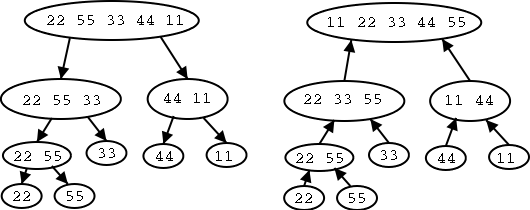
\includegraphics[width=\columnwidth]{immagini/merge_sort}
	\caption[Merge sort]{Rappresentazione dell'algoritmo merge sort.}
	\label{fig:merge}
\end{figure}

	\section{Programma}
Il \emph{programma} è un oggetto che si può presentare sotto varie forme. Le più importanti sono tre:
\begin{description}
	\item[In corso d'esecuzione.] In questo caso, prende il nome di \emph{processo};
	\item[File eseguibile.] Esso è essenzialmente un file (con estensione \ext{.exe} in \os{Windows}) contenente un insieme d'istruzioni comprensibili dall'unità di calcolo. Una volta eseguito, si traduce in un processo. Il linguaggio in cui è scritto tale file prende il nome di \emph{assembly} o \emph{linguaggio macchina}. Quest'ultimo nome lascia intuire che tale file non è fatto per essere letto ed interpretato dall'uomo;
	\item[Codice sorgente.] Questo è un file di testo contenente istruzioni comprensibili anche all'uomo. \`E scritto in un \emph{linguaggio di programmazione} (vedi il paragrafo~\ref{subsec:programmazione} a pagina~\pageref{subsec:programmazione}). Per ottenere un file eseguibile dal codice sorgente, c'è bisogno di ``tradurre'' quest'ultimo tramite un processo che, per ragioni storiche, prende il nome di \emph{compilazione}.\footnote{Per maggiori dettagli, si rimanda a degli appunti sul sito del prof.~Bernardinello all'indirizzo \url{http://www.mc3.disco.unimib.it/lif/Dep/vigcc.pdf}}.
\end{description}
	\chapter[Lezione II]{Lezione II\newline\small{\emph{31/03/2011}}}
	\section{Struttura generale di un calcolatore}
	\label{sec:neu}
\begin{figure}
	\centering
		\subfloat[John Von Neumann][{\em John Von Neumann (Budapest, 28 dicembre 1903 - Washington, 8 febbraio 1957).}\label{fig:vn}]{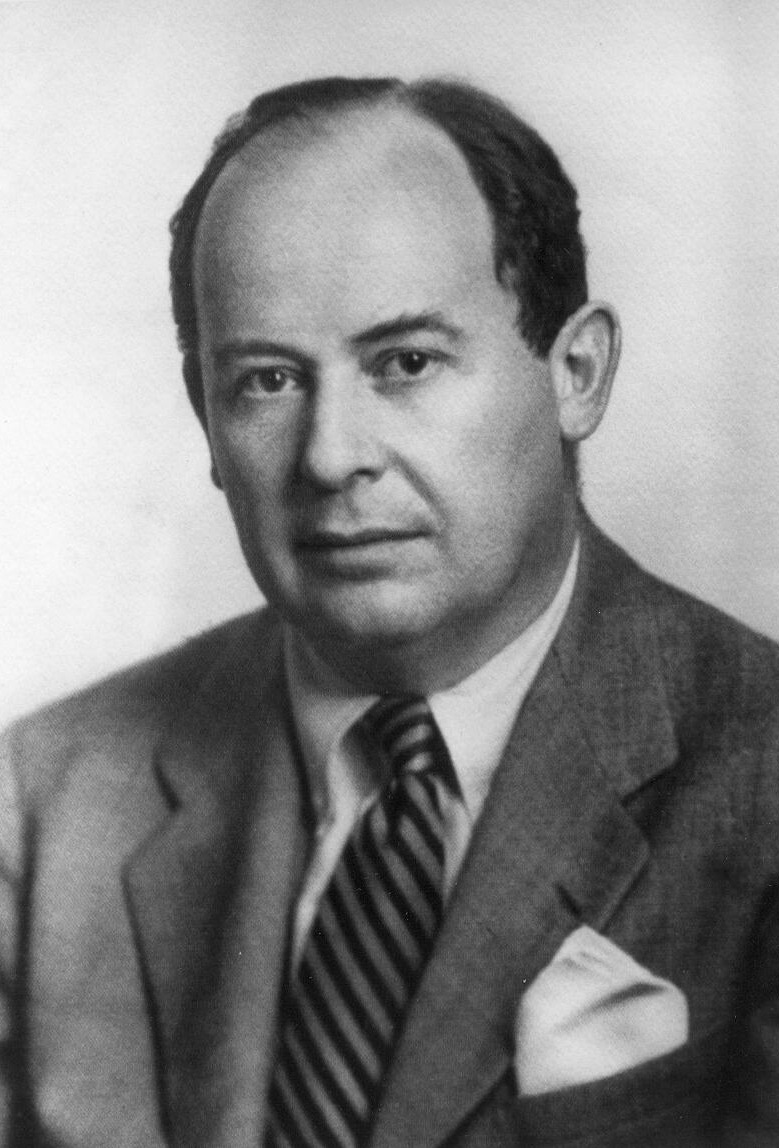
\includegraphics[width=0.45\columnwidth]{immagini/von_neu}} \quad
		\subfloat[Calcolatore di von Neumann][{\em Struttura generale di un calcolatore di von Neumann.}\label{fig:neu}]{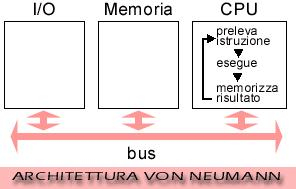
\includegraphics[width=0.45\columnwidth]{immagini/von_neumann}}
	\caption{John Von Neumann}
\end{figure}

La\marginpar{Struttura di John von Neumann} struttura di un calcolatore descritta di seguito è rimasta più o meno immutata nel corso del tempo, sin dagli anni '40. Essa è stata attribuita al matematico e informatico \emph{John von Neumann} (figura~\vref{fig:vn}). Il calcolatore (figura~\vref{fig:neu}) è essenzialmente composto da:
\begin{description}
	\item
[\ac{cpu}] Nella \ac{cpu} (ovvero \emph{Unità Centrale d'Elaborazione}) vengono  trasformati e manipolati i dati;
	\item
[\ac{ram}] La \ac{ram} (ossia la \emph{Memoria di Lavoro}) è una memoria volatile: nel caso di spegnimento del computer, i dati contenuti in essa vanno perduti.
Serve per conservare i dati durante l'esecuzione di un programma (o l'elaborazione degli stessi);
	\item
[\ac{io}] Le unità di \ac{io}, cioè d'\emph{Ingresso/Uscita} consentono di immettere/acquisire dati nel/dal calcolatore e sono, ad esempio, tastiera (input), mouse (input), monitor (output), stampante (output), etc\dots
	\item
[Memoria Permanente] ossia quei supporti che conservano i dati a lungo termine, anche dopo lo spegnimento del calcolatore. Sono, ad esempio, dischi fissi, floppy, Compact Disc, etc\dots
\end{description}


Le prime tre componenti elencate sono assolutamente \emph{necessarie} ai fini del funzionamento del calcolatore e comunicano tra loro per mezzo del \emph{bus}\index{bus}.
Affinché le varie parti lavorino in modo sincrono, inoltre, in ogni macchina è presente il \emph{clock}\index{clock}, un apparecchio simile ad un metronomo che manda dei segnali ad ogni parte del computer.
Il clock, quindi, stabilisce la frequenza di lavoro.



La \ac{cpu} contiene dei registri.
In ognuno di essi si possono conservare dei dati, che la \ac{cpu} è in grado di leggere ed utilizzare.
La \ac{ram}, in modo analogo, è organizzata in celle indicizzate da un numero intero non negativo.
Tali numeri sono progressivi e vanno da $0$ a $n$.
Affinché i programmi vengano eseguiti, è necessario memorizzare informazioni nella memoria di lavoro.
Queste sono composte, in genere, sia dai dati da elaborare, sia dalle istruzioni tramite cui avverrà l'elaborazione.

La \marginpar{Funzionamento della \ac{cpu}} macchina (più strettamente parlando, la \ac{cpu}) per funzionare esegue tre operazioni principali:
\begin{description}[]
	\item
[Fetch\index{fetch}] reperisce nella memoria di lavoro la prossima istruzione da eseguire. Tra i registri della \ac{cpu}, infatti, ve n'è uno dedicato a contenere il numero della cella (chiamato anche \emph{indirizzo}) della \ac{ram} contenente l'istruzione successiva;
	\item
[Decode\index{decode}] una volta trovata l'istruzione da eseguire è necessario che questa venga decodificata dalla \ac{cpu};
	\item
[Execute\index{execute}] avvenuta la decodifica, la \ac{cpu} esegue l'istruzione. In generale, ciò comporta una modifica del contenuto dei registri. In particolare, cambierà almeno il contenuto del \emph{program counter}\index{program counter} (il registro della \ac{cpu} che contiene l'indirizzo dell'istruzione successiva).
\end{description}

	\section{Rappresentazione della memoria del calcolatore e tipi di dato semplici}
	\label{sec:mem}
Può tornare utile immaginare la memoria di un computer come un foglio a quadretti (per gli attuali calcolatori, anche quelli presenti in ambienti domestici, il numero di ``quadretti'' è dell'ordine di \num{e9}). Ogni quadretto può contenere uno ed un solo ``dato semplice'' (ad esempio un carattere, un numero, o un qualsiasi altro \emph{simbolo}).

Ogni dato (qualsiasi) occupa una certa quantità di quadretti (o celle).
Ognuna di queste celle è identificata da un numero progressivo (il suddetto \emph{indirizzo}).\footnote{Il calcolatore non è in grado di ``comprendere'' la numerazione decimale. Esso è in grado di codificare solo istruzioni che gli vengano passate in linguaggio binario.}
Poiché spesso è abbastanza scomodo usare gli indirizzi per individuare la posizione dei dati, possiamo contrassegnare uno o più quadretti consecutivi con un nome simbolico.
In\marginpar{Variabili} questo modo, identifichiamo dei ``blocchi'' di quadretti  chiamati \emph{variabili}\index{variabile}. Le variabili vengono classificate in \emph{tipi}\index{tipo}.

Il concetto di tipo, non è una caratteristica di tutti i \emph{linguaggi di programmazione}.
In linguaggio \lang{C} è necessario specificare il tipo di una variabile ma lo stesso non vale, ad esempio, per linguaggi come il \lang{Python}.
Ad ogni tipo di dato corrisponde una particolare quantità di memoria che il calcolatore \emph{alloca} (alcuni tipi richiedono più celle di altri).

I \marginpar{Tipi primitivi} \emph{tipi primitivi}\index{tipo!primitivo} in linguaggio \lang{C} sono:
\begin{itemize}
	\item
\lstinline!char!: indica un carattere (lettera , cifra, segno…) ed occupa una cella;
	\item
\lstinline!int!: indica un numero intero (anche negativo, cioè appartenente a $\mathbb{Z}$);
	\item

\lstinline!float!: indica un numero decimale. Questa dovrebbe essere la rappresentazione di un numero reale all'interno del calcolatore. Tuttavia, per evidenti motivi, non ci è possibile memorizzare un numero con infinite cifre dopo la virgola. Per cui, il tipo \lstinline!float! fornisce una rappresentazione approssimata di un numero irrazionale (o razionale periodico).
\end{itemize}

	\section{Programmazione imperativa ed assegnamenti}
Esistono diversi \emph{paradigmi}\index{paradigma} (schemi generali) di programmazione.
Qui ci occuperemo della \emph{programmazione imperativa}.
In \marginpar{Assegnamento} questo tipo di programmazione l'operazione principale è l'\emph{assegnamento}\index{assegnamento}, definito come il processo di inserimento dei dati nelle celle.
Un esempio d'istruzione di assegnamento è la scrittura ``\lstinline!x = 5303;!'' (in linguaggio \lang{C}).
Un'istruzione d'assegnamento è formata da tre parti:
\begin{itemize}
	\item
Nome della variabile (ad esempio, ``\lstinline!x!'');
	\item
Operatore di assegnamento ``\lstinline!=!'';
	\item
Valore della variabile (ad esempio \lstinline!5303!) che deve essere \emph{compatibile} con il suo tipo, altrimenti il computer segnalerà che c'è un errore.\footnote{Le variabili di tipo \lstinline!float! ``contengono'' un numero decimale.
Si tenga presente che un assegnamento per una variabile di questo tipo dev'essere, ad esempio, \lstinline!f = 23.934;!.
La virgola è di tipo \emph{anglosassone}.
Il computer non riconoscerà un assegnamento del tipo \lstinline!f = 23,934;!.
}
\end{itemize}
Sono ammessi assegnamenti anche del tipo ``\lstinline!v = x;!'', sempre a patto che le variabili \lstinline!v! e \lstinline!x! abbiano dei tipi compatibili tra di loro.
Con questo assegnamento, anche la variabile \lstinline!v! ora ha il valore \lstinline!5303!.

Le variabili possono anche essere delle funzioni (matematiche) come, ad esempio, ``\lstinline!y = v/10;!''.
Se \lstinline!v! è un intero (poniamo \lstinline!58!), il risultato sarà un intero (\lstinline!5!).
Se, invece, \lstinline!v! è di tipo \lstinline!float!, allora otterremo come risultato \lstinline!5.8!.
Possiamo anche scrivere degli assegnamenti in cui la stessa variabile compare da entrambe le parti.
Ad esempio, ``\lstinline!x = x+1;!'' è un assegnamento valido.
Questo non fa altro che aggiornare il valore della variabile \lstinline!x!.

Supponiamo ora di avere una variabile \lstinline!beta! che sia stata dichiarata, ad esempio, di tipo \lstinline!float!.
Ammettiamo che essa contenga un certo valore e che noi vogliamo triplicare tale valore.
Possiamo, in questo caso, scrivere ``\lstinline!beta = 3 * beta;!''.
Ciò è lecito: anche se \lstinline!3! non è di tipo \lstinline!float!, la quantità \lstinline!3 * beta! lo sarà. 

Per \marginpar{Dichiarazione} comunicare al computer il tipo di variabile che intendiamo usare, dobbiamo effettuare la già citata operazione di \emph{dichiarazione}\index{dichiarazione}.
In \lang{C}, essa assume la forma ``\lstinline!float gamma;!'', oppure:
\begin{lstlisting}
float beta, gamma;
gamma = 1.0;
beta = gamma + 5;
\end{lstlisting}
In generale, tutte le dichiarazioni vanno poste all'inizio del programma

Il \lang{C} dispone anche di operatori aritmetici. I \marginpar{Principali operatori algebrici} principali operatori sono: \lstinline!+! (operatore somma), \lstinline!-! (operatore differenza), \lstinline!*! (operatore prodotto), \lstinline!/! (operatore quoziente), \lstinline!%! (operatore modulo, restituisce il resto di una divisione). Ad esempio:
\begin{lstlisting}
int z;
z = 5%3;
\end{lstlisting}
restituisce un valore \lstinline!z = 2!.

	\section{Strutture di controllo}
	\label{sec:ContStruc}
L'ordine con cui vengono eseguite le istruzioni dipende dalle \emph{strutture di controllo}.
Esse sono, essenzialmente, gli assegnamenti ed altre poche istruzioni ed hanno il compito di ``gestire'' e, appunto, controllare il flusso delle informazioni durante l'esecuzione di un programma.
Qualunque algoritmo può essere espresso per mezzo di tre strutture di controllo:
\begin{itemize}
	\item
Sequenza;
	\item
Scelta;
	\item
Iterazione.
\end{itemize}

		\subsection{Sequenza}
La \emph{sequenza} è determinata dall'ordine in cui vengono scritte le istruzioni. Per convenzione, la ``lettura'' avviene dall'alto in basso e da sinistra verso destra. Così, istruzioni scritte ``in alto'' verranno eseguite prima di istruzioni scritte ``in basso''.

		\subsection{Scelta}
In \lang{C}, la scelta si riconosce dalla preposizione \lstinline!if!. Ad esempio:

\begin{lstlisting}
if ( x < 0 )
	x = -x;
\end{lstlisting}
Sintatticamente, le parentesi tonde sono obbligatorie.
Esse racchiudono la condizione che deve essere verificata affinché il \emph{corpo} della scelta venga eseguito.
La condizione viene talvolta chiamata \emph{test}\index{test}.
Se la condizione non è verificata, l'istruzione ``\lstinline!x = -x;!'' (che nel nostro caso rappresenta il corpo della scelta) non viene eseguita.
Si noti che è possibile trovare corpi che comprendano più di una istruzione.
In questo caso, tali istruzioni vanno incluse tra parentesi graffe.
Se ne vedranno degli esempi in seguito.

Per \marginpar{Operatori relazionali} il test, si dispone dei seguenti operatori relazionali: \lstinline!<! (operatore minore), \lstinline!<=! (operatore minore o uguale), \lstinline!>! (operatore maggiore), \lstinline!>=! (operatore maggiore o uguale), \lstinline!==! (operatore uguale), \lstinline?!=? (operatore diverso\footnote{In generale, il simbolo \lstinline?!? nei test equivale ad una negazione. Quindi \lstinline?!=? starebbe a significare ``non uguale'', cioè diverso.}).


\begin{code}
\begin{minipage}{0.45\columnwidth}
	\begin{lstlisting}[caption={\ },nolol]
if ( x < 0 )
	x = -x;
else
	x = x+3;
	\end{lstlisting}
\end{minipage}	\hfill
\begin{minipage}{0.45\columnwidth}
	\begin{lstlisting}[caption={\ },nolol]
if ( x < 0 )
	x = -x;
else
	x = x+3;
	\end{lstlisting}
\end{minipage}	\hfill
\begin{minipage}{0.45\columnwidth}
	\begin{lstlisting}[caption={\ },nolol,label={code:corpo}]
if ( x < 0 ) {
	x = -x;
	y = 3+z;
	e = y+1;
}
else
	...
	\end{lstlisting}
\end{minipage}	\hfill
\begin{minipage}{0.45\columnwidth}
\begin{lstlisting}[caption={\ },nolol]
if (test1)
	if (test2)
		...
	else
		...
else
	...
	\end{lstlisting}
\end{minipage}	\hfill
\begin{minipage}{0.45\columnwidth}
	\begin{lstlisting}[caption={\ },nolol]
if (test1) 
...
else
	if (test2)
		...
	else
		...
	\end{lstlisting}
\end{minipage}	\hfill
\begin{minipage}{0.45\columnwidth}
	\begin{lstlisting}[caption={\ },nolol]
if (test1) 
...
else if (test2)
		...
	else
		...
	\end{lstlisting}
\end{minipage}
\caption{Sintassi della scelta \lstinline!if (...)  else!}
\label{riq:IfChoose}
\end{code}
È possibile trovare anche scelte che presentano le sintassi elencate nel riquadro~\vref{riq:IfChoose}. Nel codice~\vref{code:corpo}, il corpo della scelta \lstinline!if! è composto da tutte le istruzioni contenute tra parentesi graffe. Il calcolatore le esegue come se fossero una sola istruzione (naturalmente, rispettando la convenzione di eseguire prima quelle scritte  ``in alto'').

In \marginpar{Struttura caratteristica di un programma in \lang{C}} generale, un programma scritto in \lang{C} ha una struttura generale caratteristica. Essa si ripresenta quasi uguale nella maggior parte dei programmi ed è mostrata nel codice~\vref{cod:GenProSyn}.
\begin{lstlisting}[caption={[\em Struttura di un programma in linguaggio \lang{C}.] {Struttura generale di un programma in linguaggio \lang{C}.}},float,label={cod:GenProSyn}]
#include <stdio.h>

int main (void) {
	int x, y;
	float z, f;

	/* istruzioni */

	exit(...);
}
\end{lstlisting}
%	\chapter[Lezione III]{Lezione III\newline\small{\emph{07/04/2011}}}
	\subsection{Iterazione}
	\label{sec:it}

\emph{Iterazione} vuol dire \emph{ripetizione}. Possiamo individuare due tipi di iterazioni. Più esattamente, la condizione verificata la quale un'iterazione continua può essere di due tipi:
\begin{itemize}
	\item
L'iterazione viene ripetuta un numero $n$ di volte fissato a priori;
	\item
Il numero di volte $n$ per cui si ripete l'operazione viene determinato da come procede l'esecuzione (o l'iterazione stessa).
\end{itemize}	
Nel linguaggio C, non esiste una forma che equivalga alla locuzione “"ripeti l'operazione per $n$ volte'', ma bisogna ricorrere ad un'iterazione regolata da una determinata condizione.

Un espediente piuttosto frequente è mostrato nel codice~\vref{cod:conv}. Si dichiara una variabile di tipo \lstinline!int!. Si fa in modo che, ad ogni iterazione, tale variabile venga incrementata di un certo numero (ad esempio, di \lstinline!1!). Tale \marginpar{Contatore} variabile fungerà, effettivamente, da \emph{contatore}. Si fissa la condizione per la continuazione dell'iterazione (o \emph{ciclo}) in modo tale che, quando il contatore raggiunge un dato valore, il ciclo si blocchi.
\begin{lstlisting}[caption={{\em Tabella di conversione \euro{} - \pounds.}}, label={cod:conv}]
...
/* 
** dichiaro la variabile (contatore) e la ini-
** zializzo, assegnandole un  valore iniziale
*/
int i = 0; 
while ( i < 10 ) {
	printf("%d ... %f", i, i*1936.27);
	/* incremento il valore del contatore */
	i = i + 1; 
}
...
\end{lstlisting}
L'iterazione, nel codice esempio~\vref{cod:conv}, procederà finché la variabile \lstinline!i! non avrà assunto il valore \lstinline!10! (quindi, il ciclo si ripeterà 10 volte\footnote{Un errore molto frequente è impostare un ciclo di questo tipo dimenticandosi d'incrementare il contatore. Questo produrrebbe un ciclo infinito. Inoltre, il calcolatore non ha alcun modo di accorgersi di siffatti errori (si veda il paragrafo~\vref{subsec:ins}).}). In questo esempio, \marginpar{Il ciclo \lstinline!while!}il ciclo è stato introdotto introdotto usando la locuzione:
\begin{lstlisting}
while (test) {
	...
}
\end{lstlisting}
Essa inizializza un ciclo che  procede finché il test espresso tra parentesi rimarrà verificato. Quando la condizione \lstinline!i < 10! diventa falsa, l'esecutore salta il blocco \lstinline!while! e procede con il comando che segue.

Le condizioni possono anche essere concatenate, cioè è possibile specificare più test all'interno di una sola coppia di parentesi tonde. Il C dispone degli \emph{operatori logici} elencati nella tabella~\vref{tab:lop}.

\begin{table}[p]
	\centering
	\caption{Operatori logici nel linguaggio C}
	\label{tab:lop}
	\begin{tabular}{lcl}
		\toprule
Condizione &Operatore &Esempio \\
		\midrule
$C_1$ e $C_2$   &\lstinline!&&! &\lstinline!( x >= 0 && x <= 10 )! \\
$C_1$ o $C_2$   &\lstinline!||!   &\lstinline!( x <= 0 || x >= 10 )! \\
Non $C_1$	       &\lstinline?!?    &\lstinline?( !(  x > y ) )? cioè \lstinline?( x < y )?\\
		\bottomrule
	\end{tabular}
\end{table}

Nel codice~\vref{cod:conv} è stato\marginpar{Commenti} introdotto l'uso dei \emph{commenti}. Un programma scritto in C può presentare dei commenti, parti di codice che il compilatore non cerca d'interpretare. Essi sono compresi tra \emph{slash} ed \emph{asterischi} (\lstinline!/* commento */!) ed hanno lo scopo di migliorare la leggibilità del sorgente. Si può commentare il codice anche usando la forma \lstinline$// commento$. La differenza tra le due forme è che, mentre nella prima il commento finisce dopo {\color{green}\lstinline!*/!}, nella seconda tutti i caratteri su una stessa riga (da \lstinline!//! in poi) vengono ignorati al momento dell'esecuzione.

Il frammento di codice~\vref{cod:conv}, se opportunamente completato, stampa a schermo due colonne. A sinistra un numero intero da \lstinline!0! a \lstinline!9!, a destra lo stesso numero moltiplicato per \lstinline!1936.27! (una tabella di conversione tra \euro{} e \pounds). La funzione che stampa a schermo è \lstinline$printf();$\marginpar{\lstinline!printf();!}. Tale funzione può essere usata in diverse forme, riassunte nella tabella~\vref{tab:printf}.
\begin{table}[p]
	\caption{Usi della funzione \lstinline$printf();$.}
	\label{tab:printf}
	\centering
	\begin{tabular}{lp{0.4\columnwidth}}
		\toprule
Sintassi							& Funzione \\
		\midrule
\lstinline!printf("testo \n");!					& Stampa un messaggio letteralmente. La combinazione \lstinline$\n$ equivale al carattere ""a capo''. \\

\lstinline!printf("%d", num);!					& Stampa il valore della variabile \lstinline$num$, che dev'essere di tipo \lstinline$int$. \\

\lstinline!printf("%f", x);!					&  Stampa il valore della variabile \lstinline$x$, che può essere di tipo \lstinline$double$ (in questo caso, la sintassi prevederebbe \lstinline$%lf$ e non \lstinline$%f$ tra virgolette) o \lstinline$float$.\\

\lstinline!printf("testo: %8.2f", x);!		&  Ogni sotto espressione introdotta da \lstinline!%! indica il punto in cui sarà inserito il valore di una variabile. La sequenza compresa tra virgolette è seguita dall'elenco delle variabili cui si fa riferimento, separate da virgole. La combinazione \lstinline$%8.2f$ specifica che il valore della variabile \lstinline$x$ va stampato in modo che occupi almeno otto posizioni, delle quali due devono seguire il punto decimale. \\
		\bottomrule
	\end{tabular}
\end{table}

Per leggere un valore inserito nello \emph{standard input} (\lstinline!stdin!), che nella maggior parte dei casi è la tastiera, si può usare la funzione \lstinline$scanf();$\marginpar{\lstinline!scanf();!}. Tale funzione ammette le sintassi elencate nella tabella~\vref{tab:scanf}. In tutti i casi il carattere \lstinline!&! precede l'identificatore della variabile.
\begin{table}[p]
	\caption{Usi della funzione \lstinline$scanf();$.}
	\label{tab:scanf}
	\centering
	\begin{tabular}{lp{0.6\columnwidth}}
		\toprule
Sintassi							& Funzione \\
		\midrule
\lstinline!scanf("%d", &n);!				& Legge un valore di tipo \lstinline!int! e lo assegna alla variabile \lstinline!n!, che naturalmente dev'essere stata dichiarata di tipo intero. \\

\lstinline!scanf("%f", &x);!				& Legge un valore decimale e lo assegna alla variabile \lstinline!x!, che dev'essere stata dichiarata di tipo \lstinline!float!. \\

\lstinline!scanf("%lf", &y);!				& Legge un valore di tipo decimale e lo assegna alla variabile \lstinline!y!, che dev'essere stata dichiarata di tipo \lstinline!double!. \\
		\bottomrule
	\end{tabular}
\end{table}

\begin{table}[p]
	\centering
	\caption[Opzioni di  \lstinline!printf();! e \lstinline!scanf();!]{Opzioni delle funzioni  \lstinline!printf();! e \lstinline!scanf();!}
	\label{tab:spop}
	\begin{tabular}{l p{0.51\columnwidth}}
		\toprule
Opzione	&Funzione	\\
		\midrule
\lstinline!%d!	& Stampa/legge variabili di tipo \lstinline!int!.		\\
\lstinline!%f!		& Stampa/legge variabili di tipo \lstinline!float!.		\\
\lstinline!%lf!	& Stampa/legge variabili di tipo \lstinline!double!.	\\
\lstinline!%c!		& Stampa/legge variabili di tipo \lstinline!char!.		\\
\lstinline!%s!		& (Con \lstinline!scanf()!)
			    Legge stringhe di caratteri e le salva in un array.			\\
		\bottomrule
	\end{tabular}
\end{table}

	\section{Strutture Dati}
Una \emph{struttura dati}\footnote{L'espressione ""struttura dati'' è grammaticalmente scorretta in italiano. La forma corretta sarebbe ""struttura dei dati''. Tuttavia, essa è una forma ereditata dall'inglese \emph{data structures}, quindi viene accettata anche nella prima forma.} è un'entità usata per organizzare un insieme di dati all'interno della memoria del computer (ed eventualmente per memorizzarli in una memoria di massa). Detto in parole povere, è una rappresentazione schematica dei dati su cui s'intende lavorare.
La scelta delle strutture dati da utilizzare è strettamente legata a quella degli algoritmi.

		\subsection{Vettori}
		\label{subsec:array}
Il \emph{vettore} (o array) è un ""oggetto'' formato da una sequenza di valori omogenei (ossia, dello stesso tipo), una variabile in cui tutti i valori occupano posizioni adiacenti. Se si deve risolvere un problema che viene naturalmente rappresentato sotto forma vettoriale (o matriciale) questa struttura dati risulta estremamente utile. Per dichiarare un vettore, si usa la seguente sintassi: \lstinline!double p[3];!.

Si supponga di aver bisogno di rappresentare la posizione di un punto (rispetto all'origine di un sistema d'assi cartesiani orientato) nello spazio tridimensionale. Risulta comodo usare un vettore che contenga dei valori Reali\footnote{La migliore approssimazione che ottenibile di un numero $n\in\mathbb{R}$, è una variabile di tipo \lstinline!double!.}, come quello dichiarato poc'anzi, di nome \lstinline!p!, che comprende tre variabili.

Di fatto, tale dichiarazione corrisponde a quella di tre variabili: \lstinline!p[0]!, \lstinline!p[1]!, \lstinline!p[2]! (tutte di tipo \lstinline!double!). Esse occupano posizioni contigue in memoria e condividono una parte del nome (oltre ad essere indicizzate). Volendo, possono anche essere usate separatamente come delle normali variabili. L'averle dichiarate sotto forma di un vettore permette di manipolarle meglio per operazioni vettoriali.

Nel seguente codice esempio, dopo aver dichiarato un vettore di lunghezza \lstinline!100!, s'assegna alla sua $e$-esima coordinata il valore $e^2-3e$.
\begin{lstlisting}
int v[100], e;
e = 0;
while ( e <= 99 ) {
	v[e] = e*e-3*e;
	e = e + 1;
}
\end{lstlisting}

	\section{Funzioni}
In matematica, una \emph{funzione} (o \emph{applicazione}) $f$ è una \emph{relaizone} definita da:
\begin{itemize}
	\item
Un insieme $X$ detto \emph{Dominio} della funzione $f$;
	\item
Un insieme $Y$ detto \emph{Codominio} della funzione $f$;
	\item
Una legge tale per cui $\forall x \in X, \exists! \ y \in Y \mid y=f(x)$.
\end{itemize}

Si consideri una funzione tale che:
\[
y=
\begin{sistema}
abs:\mathbb{R}\mapsto\mathbb{R} \\
abs(x)=\abs{x}
\end{sistema}
\]
All'interno di un programma, si possono definire delle parti di codice che eseguono delle operazioni specifiche (\emph{funzioni}, appunto). Per fare ciò, bisogna specificare un Dominio, un Codominio e la forma della funzione (la sequenza di istruzioni che la compongono). Successivamente, la funzione sarà disponibile per essere richiamata in altre parti del programma.

Il codice~\vref{cod:absfunc} mostra la precedente funzione stesa in linguaggio C. Si noti che, dopo averla dichiarata, la si può richiamare come a riga 16. Si tenga inoltre presente che ogni programma in C \emph{deve} contenere una funzione \lstinline!main()!.
\begin{lstlisting}[caption={\em Definizione e chiamata della funzine \lstinline!abs()!.}, label={cod:absfunc}]
/* codominio_nome della funzione_(dominio) */
double abs ( double x ) {
	/*
	** Il corpo di una funzione va sempre posto
	**fra parentesi graffe.
	*/
	if ( x < 0 )
		return -x;
	else
		return x;
}

int main ( int argc, char *argv[] ) {
	double v, y;
	scanf("%lf", &v);
	y = abs(v);
	printf("%lf", y);
	exit(EXIT_SUCCESS);
}
\end{lstlisting}

Si considerino delle funzioni con due (o più) parametri formali, come la seguente:
\[
\begin{sistema}
max:\mathbb{R}\times\mathbb{R}\mapsto\mathbb{R} \\
max(x,y)=
		\begin{cases}
x,	& \text{ se } x>y \\
y,	& \text{ se } x<y
		\end{cases}
\end{sistema}
\]
Essa trova il massimo tra due numeri. Il codice~\vref{cod:MultiArgFunc}, ne mostra la stesura in C.
\begin{lstlisting}[caption={\em Funzione \lstinline!max()!, con due argomenti.}, label={cod:MultiArgFunc}]
double max ( double x, double y ) {
	if ( x < y )
		return y;
	else
		return x;
}
\end{lstlisting}
%	\chapter[Lezione IV]{Lezione IV\newline\small{\emph{14/04/2011}}}
	\section{Esercizio}
Si vuole calcolare il valore di $\pi$. \`E noto che:
\[
\frac{\pi}{4}=\sum_{k=0}^{+\infty}\frac{(-1)^k}{2k+1}=1-\frac{1}{3}+\frac{1}{5}\dots
\]
Questo metodo \emph{non} può essere steso come algoritmo (che è \emph{finito} per definizione).\footnote{Un algoritmo è un procedimento che consente di ottenere un risultato eseguendo, in un determinato ordine, dei passi semplici (scelti da un insieme finito). Pertanto:
\begin{itemize}[noitemsep]
	\item
La sequenza di istruzioni deve essere finita (\emph{finitezza});
	\item
Essa deve portare ad un risultato (\emph{effettività});
	\item
Le istruzioni devono essere eseguibili materialmente (\emph{realizzabilità});
	\item
Le istruzioni devono essere espresse in modo non ambiguo (\emph{non ambiguità});
\end{itemize}   
I passi costituenti di un algoritmo devono essere ``semplici'', nel senso di ``non ambigui''.}
Tuttavia, ci si può accontentare di approssimazioni di $\pi$ che discostino dal valore reale per una quantità finita piccola a piacere facendo eseguire al calcolatore un numero finito (se pur molto grande) di iterazioni.
La sommatoria, allora, diverrà:
\[
\frac{\pi}{4} \thickapprox \sum_{k=0}^{n\in\mathbb{N}}(-1)^k\frac{1}{2k+1}=1-\frac{1}{3}+\frac{1}{5}\dots+\frac{\ (-1)^n}{2n+1}.
\]

Un algoritmo come quello del codice~\vref{cod:pigreco} calcolerà un valore approssimato di $\pi$.
Chiaramente, la precisione del valore calcolato dipenderà dalla grandezza di $n$.
Infatti
\[
\lim_{n\to\infty}\sum_{k=0}^n\frac{\ (-1)^k}{2k+1} =\frac{\pi}{4}.
\]
\begin{lstlisting}[caption={\em Calcolo del valore approssimato di $\pi$.}, label={cod:pigreco}]
#include <stdio.h>
#include <stdlib.h>
#include <math.h>

int main ( int argc, char *argv[] ) {
	int n, i = 0;
	double somma = 0.0;

	/* chiedo di inserire il numero di interazioni */
	printf("Inserisci n: ");
	scanf("%d", &n);

	/* calcolo il valore approssimato di pi / 4*/
	while ( i <= n ) {
		if ( i % 2 == 0 ) /* i pari */
			somma = somma + ( 1 / ( 2 * i + 1 ) );
		else /* i dispari */
			somma = somma - ( 1 / ( 2 * i + 1 ) );

		/* incremento il contatore */
		i = i + 1;
	}

	/* stampo il risultato */
	printf("Pi Greco = %lf", somma * 4);

	exit(EXIT_SUCCESS);
}
\end{lstlisting}

%	\chapter[Lezione V]{Lezione V\newline\small{\emph{21/04/2011}}}
	\section{Ancora sulle funzioni}
	\label{sec:fun2}
La funzione è una specie di ``scatola'' cui si associa un nome simbolico: vi entrano dei dati e ne esce il risultato della loro elaborazione.
Quest'ultima avviene per mezzo delle istruzioni che ne compongono il corpo.

In \marginpar{L'istruzione \lstinline!return!} una funzione, l'istruzione \lstinline!return! è sempre l'ultima ad essere eseguita e ne indica la fine.
Si noti che ciò non vuol dire essa che debba essere l'ultima ad essere scritta.
Se è inclusa in una scelta, ad esempio, non è affatto detto che debba essere eseguita.
\`E lecito, dunque, che dopo ``\lstinline$return $\MyComment{\dots}\lstinline$;$'' vi siano altre righe di codice.

Quando una funzione viene eseguita, il processo principale si ``blocca'' in attesa del suo risultato.
Tutte le variabili create durante questo lasso di tempo vengono cancellate quando essa termina (all'istruzione \lstinline!return!, appunto). 

Nella\marginpar{Argomenti formali e reali} definizione della funzione, le variabili che si trovano all'interno delle parentesi tonde sono dette \emph{argomenti formali}\index{argomento formale}.
Nel momento in cui la si richiama in qualche altra riga del codice, le si passano degli \emph{argomenti reali}\index{argomento reale}.
Il codice~\ref{cod:callfunc} è un esempio di chiamata della funzione \lstinline!flip()! (all'interno della funzione \lstinline!main()!).
Qui, le variabili \lstinline!a!, \lstinline!b! e \lstinline!c! sono gli argomenti reali della chiamata della funzione \lstinline!flip()!.
Si noti che essi sono stati dichiarati in modo da essere compatibili con i tipi richiesti dagli argomenti formali.
\begin{lstlisting}[caption={\em Chiamata della funzione \lstinline!flip()!.}, label={cod:callfunc}]
double flip (int x, double y, int z ) {

	£!\MyComment{istruzioni}!£

	return £!\MyComment{\dots}!£;
}

int main ( int argc, char *argv[] ) {
	int a, c;
	double b, x;

	x = flip( a, b, c );

	£!\MyComment{\dots}!£
}
\end{lstlisting}


Le\marginpar{Variabili locali e globali} variabili definite in qualsiasi funzione prendono il nome di \emph{variabili locali}\index{variabile!locale} della funzione \lstinline!x()! (dove \lstinline!x()! è il nome della stessa: \lstinline!flip()!, ad esempio).
In \lang{C}, esse si distinguono dalle  \emph{variabili globali}\index{variabile!globale} che, dichiarate al di fuori di tutte le funzioni, restano a disposizione di ognuna di esse per tutta la durata del programma---cioè della funzione \lstinline!main()!.
Ogni funzione può modificare il valore di una variabile globale ma non è possibile richiamare direttamente una variabile della funzione \lstinline!flip()! dalla funzione \lstinline!main()!, ad esempio.\footnote{Lo si può però fare tramite i puntatori (vedi il paragrafo~\ref{sec:pointers} a pagina~\pageref{sec:pointers}).}

La\marginpar{Passaggio per valore} comunicazione tra funzioni avviene tramite un procedimento chiamato \emph{passaggio per valore} (descritto nel prossimo esempio).
Una funzione riceve il valore di una variabile come parametro reale, ma \emph{non} può modificare il valore assegnato alla stessa.\footnote{Questo non è sempre vero. A causa della loro stretta relazione coi puntatori, è possibile che il valore di una variabile dichiarata come array passata come argomento reale venga modificata durante l'esecuzione di una funzione (si veda sempre il paragrafo~\ref{sec:pointers} a pagina~\pageref{sec:pointers}).}
Quando una funzione viene eseguita, il calcolatore le riserva uno spazio chiamato \emph{record di attivazione}\index{record di attivazione}.

Si supponga di voler scrivere un programma che calcola la somma dei primi $n$ elementi di un array:
\begin{lstlisting}
double somma ( double v[], int n ) {
	int i = 0;
	double s = 0.0;

	while ( i < n) {
		s = s + v[i];
		i = i + 1;
	}

	return s;
}

int main ( int argc, char *argv[] ) {
	double m[10], p[20], v, w;

	v = somma( m, 10 );
	w = somma( p, 15 );

	£!\MyComment{\dots}!£

}
\end{lstlisting}
Si noti che tale programma funziona se e solo se, quando si chiama la funzione \lstinline!somma()!, il secondo argomento è minore o uguale alla lunghezza del vettore passato come primo argomento. In caso contrario, si otterrà soltanto un \emph{errore di segmentazione}.


\begin{code}
\begin{minipage}{0.45\columnwidth}
	\begin{lstlisting}[caption={\em Il tipo \lstinline!char!.},nolol,label={code:char}]
char x;
char p[10];
p[3] = 'n';
	\end{lstlisting}
\end{minipage}	\hfill
\begin{minipage}{0.45\columnwidth}
	\begin{lstlisting}[caption={\ },nolol,label={code:Printb}]
char x = 'a';
printf("%c", x + 1);
	\end{lstlisting}
\end{minipage}
\caption{I caratteri in \lang{C}.}
\label{riq:char}
\end{code}
Il codice~\ref{code:char} nel riquadro~\ref{riq:char}, introduce ora un nuovo tipo di variabile, che corrisponde al “simbolo”.
I vettori di caratteri costituiscono la rappresentazione delle parole in \lang{C}. 
Le variabili di tipo \lstinline!char! si dichiarano racchiudendo il valore da assegnare tra singoli apici. Anche i numeri possono essere considerati dei caratteri, purché racchiusi tra apici.
Dopo aver dichiarato un numero come carattere, tuttavia, non è possibile eseguire le consuete operazioni algebriche su di esso.

Nel \marginpar{Rappresentazione dei caratteri} calcolatore, ad ogni carattere è assegnata una sequenza di cifre binarie (in genere, \num{8} cifre) che è effettivamente un numero.
Pertanto, l'espressione ``\lstinline!p[3] * 4!'' ha significato, ma non è quello che ci si aspetterebbe.
La codifica numerica dei caratteri, tuttavia, può consentire delle operazioni interessanti.
Le lettere dell'alfabeto, ad esempio, sono numerate in ordine progressivo.\footnote{Le lettere maiuscole sono poste in ordine progressivo tra di loro, così come quelle minuscole. Tuttavia, le rappresentazioni di \lstinline!a! e \lstinline!B! non hanno differiscono tra di loro per un unità.}
Con un programma simile a quello del codice~\ref{code:Printb}, il calcolatore stamperà a schermo il carattere ``b''.
Tale rappresentazione dei caratteri permette, inoltre, di ordinare alfabeticamente le parole.

		\subsection{Filtri}
L'istruzione\marginpar{La funzione \lstinline!getchar()!} ``\lstinline!x = getchar();!''\index{getchar()!\textt{getchar()}} comunica all'esecutore di leggere il carattere successivo dallo standard input (in genere, la tastiera), assegnarlo alla variabile \lstinline!x! e di toglierlo dalle serie dei ``caratteri in entrata''.
La funzione \lstinline!getchar()! non ammette parametri e ha come unico risultato l'assegnamento del carattere letto alla variabile cui è associata (nella fattispecie, \lstinline!x!).
L'\marginpar{La funzione \lstinline!putchar()!}istruzione ``\lstinline!putchar(x);!''\index{putchar()!\textt{putchar()}}, invece, stampa sullo \emph{standard output}\index{standard output} (\lstinline!stdout!\index{stdout@\texttt{stdout}}, in genere il monitor) il valore della variabile \lstinline!x!.

Il programma nel codice~\vref{cod:eco} ``fa l'eco'' di quanto riceve dallo standard input.
Esso appartiene alla famiglia dei \emph{filtri}, cioè programmi che leggono dei caratteri ed eseguono delle operazioni su di essi.
Il valore \lstinline!EOF! è una sequenza di caratteri speciale (del linguaggio \lang{C}) che sta per \emph{End Of File}.
Per i sistemi \os{UNIX}, la sequenza riconosciuta come \lstinline!EOF! è la combinazione di tasti \key{CTRL + D}. 
\begin{lstlisting}[caption={\em Esempio di filtro.}, label={cod:eco}]
#include <stdio.h>
#include <stdlib.h>
#include <ctype.h>

int main ( int argc, char *argv[] ) {
	int c;
	/* leggo il primo carattere */
	c = getchar();
	while ( c != EOF ) { /* fino a quando non premo 'CTRL + D' */
		/* stampo il carattere */
		putchar(c);
		/* leggo il successivo */
		c = getchar();
	}

	exit(EXIT_SUCCESS);
}
\end{lstlisting}
%	\chapter[Lezione VI]{Lezione VI\newline\small{\emph{28/04/2011}}}
	\section{Strutture Dati}
		\subsection{Grafo}
		\label{subsec:grafo}
Un \emph{grafo} (figura~\vref{fig:grafo}) è un oggetto $G = (V, E)$ composto da \emph{vertici} $v_n\in V$ e \emph{lati} $e_m\in E$. Si ha che:
\[
\begin{split}
&V=\{(x_1,y_1),\dots,(x_n,y_n)\} \\
&E\subseteq V\times V
\end{split}
\]
\begin{wrapfloat}{figure}{i}{0pt}{
	\begin{tikzpicture}
		\coordinate (A) at (0,4.5);
		\coordinate (B) at (2,4);
		\coordinate (C) at (4,5.5);
		\coordinate (D) at (4.5,3);
		\coordinate (E) at (3,2);
		\coordinate (F) at (0.5,1.5);
	
		\foreach \a/\b in {A/B, B/C, C/E, E/F, A/F, A/E}
			\draw [line width=0.5pt, color=blue] (\a) -- (\b);
	
		\foreach \n in {A,B,C,D,E,F} 
			\draw [] node [circle,draw,minimum size=1cm,top color=gray] at (\n) {\color{black}{\n}};
	\end{tikzpicture}
}
%	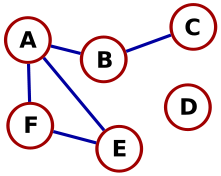
\includegraphics[width=0.5\columnwidth]{immagini/grafo}
	\caption{Esempio di grafo.}
	\label{fig:grafo}
\end{wrapfloat}
L'insieme dei lati è un sottoinsieme del prodotto cartesiano dei punti. Ognuno di essi è \emph{univocamente} determinato da una coppia di punti (se non è orientato). Un lato, quindi, è un segmento non orientato completamente individuato da una coppia di punti. Se consideriamo dei segmenti orientati, probabilmente, il grafo sarà una funzione di grandezze diverse. Bisogna cioè aggiungere altre informazioni.

Supponiamo di avere segmenti non orientati. Siano $v_1,v_2\in V$ per rappresentare un segmento da $v_1$ a $v_2$, allora $\overline{v_{1}v_{2}}$ e $\overline{v_{2}v_{1}}$ coincidono. Nel caso di segmenti orientati, tuttavia, possiamo stabilire, per convenzione, che il primo punto sia l'origine del segmento, il verso sia indicato dal secondo punto e che la differenza tra i vertici permetta di stabilire il modulo del vettore. Quindi, per un vettore orientato da $v_1$ a $v_2$ ci basterà scrivere $\overline{v_{1}v_{2}}$ (oppure $\overrightarrow{v_{1}v_{2}}$).

		\subsection{Strutture}
		\label{subsec:record}
Si supponga di voler creare un programma che tenga traccia della carriera scolastica di alcuni studenti. Innanzitutto, bisogna cercare di selezionare i dati essenziali ai fini del programma. Si può immaginare lo studente come un ente univocamente determinato da tre variabili. Si dichiarano, allora\footnote{Si può anche dichiarare \lstinline!char n_matricola[6];! ma è molto più semplice che a rappresentare la matricola sia un numero (intero).}:
\begin{lstlisting}
char nome[24];
int n_matricola;
int voti[6];
\end{lstlisting}
Queste variabili, tuttavia, sono ancora indipendenti tra di loro. Dal momento che si riferiscono ad una stessa persona, sarebbe più utile poterle trattare come se fossero tutte ""legate''. È\marginpar{Record} questo il concetto di \emph{record}. Un record permette di trattare più variabili non omogenee, come se fossero aggregate tra di loro.
\begin{lstlisting}[caption={[\em Struttura e variabili] {\em Definizione di una struttura e dichiarazione di variabili.}}, label={cod:struct}]
struct studente {
	char nome[24];
	int matricola, voti[6];
} maria, antonio;

int main ( int argc, char *argv[] ) {
	struct studente giuseppe, giovanni;
	...
}
\end{lstlisting}
Nella fattispecie, il record \lstinline!studenti! contiene tre \emph{campi}. Nel linguaggio C, il record prende il nome di \emph{struttura}. La definizione delle strutture segue generalmente le prime direttive in cima al codice sorgente (\lstinline!#include <...>!) in modo che risulti ben visibile. Si noti che dichiarare una struttura equivale, di fatto, a definire un nuovo tipo di variabile.

Nel codice~\vref{cod:struct} \lstinline!studente! è l'\emph{identificatore} (o \emph{tag}) della struttura\footnote{Non è strettamente necessario introdurre la tag ma, per motivi di leggibilità, è fortemente consigliato.}. All'interno delle parentesi graffe (obbligatorie) si dichiarano le variabili che formeranno i campi della struttura. \`E possibile dichiarare delle variabili di tipo \lstinline!struct studente! immediatamente dopo la definizione della struttura (come \lstinline!maria! e \lstinline!antonio! nel codice~\vref{cod:struct}). Alternativamente, è consentito farlo in qualsiasi altra riga di codice, usando la sintassi descritta nel codice~\vref{cod:struct} per la dichiarazione di \lstinline!guseppe! e \lstinline!giovanni!.

Il linguaggio C consente\marginpar{\lstinline!typedef!} di assegnare un ""sinomimo'' a \lstinline!struct studente! tramite la funzione \lstinline!typedef tipo_1 tipo_2;!:
\begin{lstlisting}[caption={\em \lstinline!typedef! e assegnamenti.}, label={cod:strass}]
typedef struct studente Studente;

int main ( int argc, char *argv[] ) {
	Studente maria, antonio;
	maria.matricola = 73659;
	maria.voti[2] = 27;
	...
}
\end{lstlisting}
In questo modo, si possono dichiarare delle variabili di tipo \lstinline!struct studente!, tramite la parola \lstinline!Studente!. Volendo richiamare (o assegnare un valore ad) un campo della struttura, la sintassi è riportata nelle righe 6 e 7 del codice~\vref{cod:strass}. La regola è: \emph{nome}.\emph{campo}\texttt{ = }\emph{valore}\texttt{;}.

Si tenga presente che, avendo dichiarato due record, \lstinline!a! e \lstinline!b!, è lecito operare un assegnamento nel modo usuale \lstinline!a = b;!. Tuttavia, non si possono confrontare due strutture con la scrittura \lstinline!a == b;!: bisogna confrontare le strutture campo per campo.

Spesso \marginpar{Direttiva \lstinline!#define!} può risultare conveniente specificare una direttiva\footnote{Le direttive \emph{non} sono istruzioni, quindi non bisogna concludere la riga con \lstinline!;!.} \lstinline!#define! all'inizio del codice sorgente come mostrato nel codice~\vref{cod:def}. Dopo aver specificato questa direttiva, il compilatore sostituirà il valore \lstinline!30! ogni qualvolta incontrerà il carattere \lstinline!L!\footnote{Il carattere deve essere una \emph{unità logica}, cioè, il compilatore non sostituirà il valore \lstinline!30! a \lstinline!L! se esso è (ad esempio) all'interno di una parola.}. Tale direttiva renderà il programma molto più facile da modificare.

Si supponga di voler creare una struttura che rappresenti un punto nello spazio bidimensionale. Oltre alla rappresentazione vettoriale, è possibile utilizzare un record composto da due campi, come nel codice~\vref{cod:ptrt}. Inoltre, poiché un rettangolo (parallelogramma retto) è univocamente individuato dagli estremi della sua diagonale, ci bastano due punti.
\begin{code}
\begin{minipage}{0.45\columnwidth}
	\begin{lstlisting}[caption={\em La direttiva \lstinline?\#define?.}, label={cod:def}]
#include <...>
#define L 30

struct nome {
	char name[L];
};
	\end{lstlisting}
\end{minipage}	\hfill
\begin{minipage}{0.45\columnwidth}
	\begin{lstlisting}[caption={\em Punto e rettangolo.}, label={cod:ptrt}]
struct punto {
	double x;
	double y;
}
struct rettangolo {
	struct punto a_sx;
	struct punto b_dx;
}
	\end{lstlisting}
\end{minipage}

\end{code}

	\section{Stringhe}
In C non esiste un tipo di variabile specifico per gestire le \emph{stringhe}\footnote{In Informatica, una stringa è una sequenza di caratteri (ad esempio, una parola).}. Le stringe vengono trattate come sequenze di caratteri. Per memorizzarle, quindi, si renderà necessario dichiarare un array di caratteri. In C, ogni stringa termina con un carattere speciale detto \emph{terminatore} (rappresentato con  \lstinline!\0!). Si noti che anch'esso occupa lo spazio di un carattere in memoria.

La\marginpar{La funzione \lstinline!strcpy();!} funzione \lstinline!strcpy(dest[], sorg[]);! copia una stringa da un array di caratteri, specificato come secondo argomento reale (\lstinline!sorg[]!), ad un altro, indicato dal primo parametro reale (\lstinline!dest[]!). Si può sfruttare tale funzione anche per effettuare un assegnamento, come nel codice~\vref{cod:strcpy}. In alternativa, è possibile usare la funzione \lstinline!scanf();! con l'opzione \lstinline!%s!
(vedi la tabella~\vref{tab:spop}) per assegnare ad un array di tipo \lstinline!char! stringhe immesse nello dallo \lstinline!stdin!.
\begin{lstlisting}[caption={\em \lstinline!strcpy();! e \lstinline!scanf();!.}, label={cod:strcpy}]
struct studente {
	char nome[24];
	int matricola, voti[6];
} maria, antonio;

int main ( int argc, char *argv[] ) {
	strcpy(maria.nome, "Maria");
	scanf("%s", &antonio.nome);
	...
}
\end{lstlisting}


	\section{Puntatori}
	\label{sec:pointers}
Come già accennato nel paragrafo~\vref{sec:mem}, ogni variabile occupa una determinata porzione di spazio e una posizione identificata da un indirizzo (che è praticamente un numero). Ora, è possibile manipolare delle variabili in due modi differenti ma equivalenti:
\begin{description}
	\item [Direttamente:]
tramite assegnamenti che operino su di esse;
	\item [Indirettamente:]
conoscendo i loro indirizzi\footnote{L'operatore \lstinline!&! restituisce l'indirizzo di una variabile. L'operatore \lstinline!*!, invece, ci permette di modificare il valore di una variabile conoscendo il suo indirizzo.}.
\end{description}
Nel codice d'esempio seguente, si è dapprima assegnato alla variabile \lstinline!p! l'indirizzo di \lstinline!x!. Successivamente si dà ad \lstinline!y! il valore di \lstinline!x! usando il suo indirizzo. Nella terza istruzione \lstinline!x! assume il valore \lstinline!0!, sempre per mezzo del suo indirizzo memorizzato nella variabile \lstinline!p!.
\begin{lstlisting}
p = &x;
y = *p;
*p = 0;
\end{lstlisting}

Si badi che nella dichiarazione di un vettore, sia esso \lstinline!int p[10];!,la lettera \lstinline!p! è, in sostanza, un puntatore alla prima variabile del vettore. In altre parole \lstinline!p! equivale a \lstinline!&p[0]!.

\begin{code}
\centering
\caption{Passaggio per valore}
\label{code:ValPass}
	\begin{minipage}{0.45\columnwidth}
\begin{lstlisting}[caption={\em \lstinline!x! non viene modificato.},label={cod:NoMod},nolol]
int function (int a, int b) {
	a = 2*b;
	...
}
int x, y;
c = function(x, y);
\end{lstlisting}
	\end{minipage}	\hfill
	\begin{minipage}{0.5\columnwidth}
\begin{lstlisting}[caption={\em \lstinline!x! viene modificato.},label={cod:Mod},nolol]
int function (int *a, int b) {
	*a = 2*b;
	...
}
int x, y;
c = function(&x, y);
\end{lstlisting}
	\end{minipage}
\end{code}
Com'è stato già detto nel paragrafo~\vref{sec:fun2}, una funzione non può modificare il valore del suo parametro reale tramite il passaggio per valore. Si consideri il riquadro~\vref{code:ValPass}.
Nel codice~\ref{cod:NoMod}, la funzione non modificherà il valore di \lstinline!x!. Nel~\ref{cod:Mod}, invece, il valore di \lstinline!x! verrà modificato anche quando la funzione sarà terminata perché la funzione ""ha accesso'' al valore di \lstinline!x! tramite il suo indirizzo.

Per quanto detto sui vettori, passando come parametro il nome di un vettore in una funzione simile il valore della variabile verrà modificato.
%	\chapter[Lezione VII]{Lezione VII\newline\small{\emph{05/05/2011}}}
	\section{Notazioni algebriche}
Si consideri una qualsiasi operazione algebrica. Fino ad ora, si sono adoperate soltanto sintassi in cui l'operatore s'inserisce tra i due operandi (ad esempio, ``$3 + 4$'').
Questo tipo di notazione si dice \emph{infissa}\index{notazione infissa}.
In questa forma, espressioni complicate o lunghe, come ``$5\cdot(3+4)$'', richiedono l'uso di parentesi.

Si prenda l'espressione ``$5\cdot\{[(9+8)\cdot(4+6)]+7\}$ in notazione infissa.
Esiste un altro modo di rappresentarla in forma \emph{postfissa}\index{notazione postfissa} (o polacca) e riscriverla come $5\ 9\ 8 + 4\ 6 + \cdot 7 + \cdot$. 
a notazione postfissa prevede, come si evince dall'esempio, che l'operatore algebrico segua i due operandi.
Nel caso più semplice, $3+4$ diventa $3\ 4 +$. L'espressione si risolve nel modo usuale:
\begin{equation*}
\begin{aligned}
5\ 9\ 8 + 4\ 6 + \cdot\, 7 + \cdot &= \\
5\ 17\ 10 \cdot 7 + \cdot &= \\
5\ 170\ 7 + \cdot &= \\
 5\ 177\, \cdot &= 885
\end{aligned}
%\end{array}
\end{equation*}


	\section{Strutture Dati}
		\subsection{Stack}
		\label{subsec:stack}
Gli aspetti caratteristici di una struttura dati dati sono:
\begin{itemize}
	\item
I valori che riesce ad assumere (quindi le grandezze che può rappresentare);
	\item
Le operazioni che posso compiere sulla struttura.

\end{itemize}
Per i tipi primitivi, le operazioni definite sono piuttosto implicite e date per scontate fino a questo momento.
In ogni caso, si tratta di operazioni algebriche di base (somma, prodotto, resto, etc\dots).
Sfruttando la notazione postfissa, è possibile creare una struttura dati che definisce un particolare procedimento per risolvere un espressione.

Si immagini \marginpar{Operazioni \lstinline!pop! e \lstinline!push!} di avere una \emph{pila}\index{pila} (in inglese, \emph{stack}\index{stack}) di dischetti.
Ogni dischetto può memorizzare uno ed un solo numero.
Sulla pila è possibile compiere solo due operazioni (vedi la figura~\ref{fig:poppush}):
\begin{itemize}
	\item
\lstinline!push:! mettere un dischetto in cima alla pila;
	\item
\lstinline!pop:! togliere un dischetto dalla cima della pila.
\end{itemize}
Questo procedimento definisce, per i dati, una disciplina del tipo \acs{lifo}, che sta per \emph{\acl{lifo}}: l'ultimo elemento inserito è il primo ad essere prelevato.

Ora, si vuole creare un algoritmo che permetta di risolvere espressioni scritte in notazione postfissa sfruttando le operazioni concesse dagli stack.
Si potrebbe immaginare di memorizzare nei dischetti i numeri immessi (\lstinline!push!) finché non si legge un operatore matematico.
A questo punto, si estraggono i due dischetti in cima alla pila (\lstinline!pop!) e si esegue su di essi l'operazione descritta dall'operatore immesso.
Successivamente, si memorizza il risultato dell'operazione su un dischetto e lo si mette in cima alla pila (\lstinline!push!).
\begin{wrapfloat}{figure}{i}{0pt}
	\centering
%	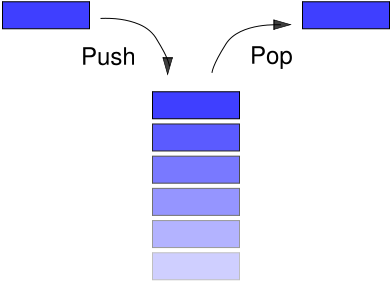
\includegraphics[width=0.4\columnwidth]{immagini/pop_push}
\begin{tikzpicture}[
	scale = 1.5,
	x={(1 cm,0 cm)},
	z={(-.35cm,-.22cm)},
	y={(0cm,1cm)}
]
\tikzset{zxplane/.style={canvas is zx plane at y=#1,very thin}}
\tikzset{yxplane/.style={canvas is yx plane at z=#1,very thin}}

%\begin{scope}[]
			\node[rotate = 90] () at (-1.3,.5) {stack};
		\begin{scope}[canvas is yx plane at z=0]
			\draw [->, shorten >=4pt] (2.5,-1.1) arc (0:90:1) node [at start,above] {\algo{pop}};
			\draw [<-,shorten >=4pt] (2.5,1.1) arc (0:-90:1) node [at start,above] {\algo{push}};

		\end{scope}

		\begin{scope}[zxplane=1.5]
			\draw[fill=black!50!blue, opacity=.3] (1,0) arc (0:360:1) ;
		\end{scope}

	\foreach \x in {0,1,...,10} {
		\begin{scope}[zxplane=\x/10]
			\draw[fill=black!50, opacity=.3] (1,0) arc (0:360:1) ;
		\end{scope}
	}
%\end{scope}

\end{tikzpicture}
	\caption[Stack]{Funzioni \algo{pop} e \algo{push} su uno stack.}
	\label{fig:poppush}
\end{wrapfloat}
\begin{table}
	\centering
	\caption[Stack]{La tabella mostra il contenuto dello stack ad ogni iterazione (tempo).}
	\label{tab:stack}
	\begin{tabular}{ l | l l l l l l l l l l l }
		\toprule
Tempo 			&0	&1 	&2 	&3 	&4 	&5 	&6 	&7 	&8 	&9 	&10	\\
		\midrule
\multirow{4}*{Pila}   	&5 	&9 	&8 	&17 	&4	&6	&10	&170	 &7 	&177	&855  \\
				&	&5	&9	&5	&17	&4	&17	&5	&170	&5	&	\\
				&	&	&5	&	&5	&17	&5	&	&5	&	&	\\
				&	&	&	&	&	&5	&	&	&	&	&	\\
	\end{tabular}
\end{table}
In questo modo\marginpar{Prototipi delle funzioni \lstinline!pop()! e \lstinline!push()!} è possibile calcolare l'espressione precedente in notazione postfissa; la tabella \ref{tab:stack} mostra i valori presenti nello stack durante l'esecuzione dell'algoritmo.

Si supponga che sia stato definito un tipo di dato \lstinline!stack! in linguaggio \lang{C}.
Si crea, allora, un prototipo della funzione \lstinline!push!: \lstinline!stack push (stack s, int v )!.
Si può assumere che la funzione \lstinline!push! riceva come argomento un numero (nella fattispecie, un intero) e lo stack su cui inserirlo, e restituisca uno stack diverso.
La funzione \lstinline!pop!, produrrebbe un nuovo stack e un intero.
Tuttavia, in \lang{C}, una funzione può produrre un solo valore.
Allora, si ricorre ad un piccolo ``trucchetto'': definendo un solo stack, tutte le funzioni possono solo lavorare su di esso e non c'è più bisogno d'inserirlo né tra gli argomenti della funzione, né nel suo codominio.

Ora, bisogna costruire un tipo di dato che permetta di rappresentare uno stack.
Esistono diverse opzioni: una delle più comode, per il momento, è costruire un array (vedi anche il paragrafo~\ref{sec:vari:stack} a pagina~\pageref{sec:vari:stack}) che, tuttavia, è una struttura dati non dinamica perché la sua lunghezza non cambia.
Si tratterà questo problema più avanti (nel paragrafo~\ref{sec:malloc()} a pagina~\pageref{sec:malloc()}).
Per ora, si assuma di aver dichiarato un array di dimensioni sufficienti per contenere tutti i dati inseriti.
Si può pensare di riempire il vettore dalla posizione più piccola (\lstinline!0!) e continuare progressivamente verso quella più grande.
Per tenete traccia del primo elemento vuoto del vettore, c'è bisogno di dichiarare una variabile ausiliaria (in questo caso di tipo \lstinline!int!).
Il codice~\ref{cod:stack} esemplifica quanto detto finora.
È importare tenere presente, tuttavia, che la funzione \lstinline!push! dà errore (di \emph{segmentazione}) se \lstinline!valori.indice! è uguale o maggiore della quantità \lstinline!N!.
Analogamente, la funzione \lstinline!pop! dà errore se il vettore \lstinline!valori.val! è vuoto.
Infatti, se \lstinline!valori.indice == 0!, la funzione \lstinline!pop! dà errore (ancora di segmentazione).
Vi si può rimediare semplicemente introducendo delle scelte.

\begin{lstlisting}[caption={[{\em Costruzione di uno stack.}]{\em Costruzione di uno stack. In questo esempio s'è usato un record per raggruppare la pila e l'intero che punta al primo elemento vuoto.}}, label={cod:stack}]
/* stack */
struct pila {
	char val[N];
	int indice;
} valori;

void push (char v) {
	valori.val[valori.indice] = v;
	valori.indice++;
}

/* senza argomenti */
char pop (void) {
	valori.indice--;
	return valori.val[valori.indice];
}
\end{lstlisting}

	\section{Allocazione dinamica della memoria}
	\label{sec:malloc()}
Si è già detto che il vettore, come tutte le strutture dati viste finora, è un modello di dati \emph{statico}. Una volta dichiarato, ha una lunghezza fissa.
In \lang{C}, tuttavia, è possibile riservare più spazio ad una o più variabili durante l'esecuzione di un programma.

La\marginpar{La funzione \lstinline!malloc()!} funzione \lstinline!malloc(size_t N)! permette di riservare \lstinline!N! \si{byte} per l'assegnamento di una variabile.
La locuzione \lstinline!size_t N! si riferisce al numero di byte che si chiede di riservare.\footnote{Un \si{byte} può contenere un carattere, con \lstinline!N! sempre strettamente maggiore di zero.
Generalmente---ma non sempre---un intero occupa \SI{4}{\byte}.}
La funzione \lstinline!malloc()! restituisce un puntatore di tipo speciale \lstinline!void! (infatti il prototipo della funzione è \lstinline!void * malloc(size_t N)!).
Questo crea un'inconsistenza formale, poiché tale tipo non corrisponde a quello del puntatore che si è dichiarato.
Anche se il calcolatore tollera tale inconsistenza, è sempre meglio operare un \emph{cast}\index{cast}, come nel codice~\ref{cod:malloc()}, specificando tra parentesi il tipo del puntatore:
\begin{lstlisting}
£!\MyComment{tipo}!£ n;
n = (£!\MyComment{tipo}!£ *) malloc( sizeof( £!\MyComment{tipo}!£ ) );
\end{lstlisting}
La funzione \lstinline!sizeof(!\MyComment{tipo}\lstinline!)!, alle righe~\ref{riga:9} e~\ref{riga:14} nel codice~\ref{cod:malloc()}, restituisce il numero di \si{byte} occupato dal \MyComment{tipo} di dato specificato come argomento.
Ad esempio, spesso si ha che \lstinline!sizeof( int )! restituisce il valore \num{4}.

La\marginpar{\lstinline!malloc()! e gli array} funzione \lstinline!malloc()! assume una forma particolarmente comoda per la dichiarazione e l'uso di array.
Nel codice~\ref{cod:malloc()}, alla riga~\ref{riga:14}, ad esempio, si chiede riservare lo spazio per \num{100} interi.
Esso sarà contiguo e quindi adatto ad essere indicizzato tramite un vettore.
La stretta relazione tra il nome di un array e i puntatori cui si è accennato in precedenza permette di effettuare degli assegnamenti come quelli nell'ultima riga.
\begin{lstlisting}[caption={[\em Uso della funzione \lstinline!malloc()!.]{\em Uso della funzione \lstinline!malloc()!. Si  faccia particolare attenzione a non dimenticare d'inserire la scelta immediatamente dopo aver richiamato tale funzione.}}, label={cod:malloc()}]
struct nodo {
	int val;
	char c;
} x, *p, *n;
int *pn;

p = &x; /* assegno a p l'indirizzo di x */
(*p).val = 0; /* assegno 0 a x.val */

n = (struct nodo *) malloc( sizeof( struct nodo ) ); £!\label{riga:9}!£
/* controllo che l'indirizzo sia valido */
if ( n == NULL )
	exit( EXIT_FAILURE );

(*n).val = 10;

pn = (int *) malloc( 100 * sizeof( int ) ); £!\label{riga:14}!£
if ( pn == NULL )
	exit(EXIT_FAILURE);

pn[10] = 1;
\end{lstlisting}
Qualora la funzione \lstinline!malloc()! non trovi abbastanza spazio contiguo da allocare, ritorna il valore \lstinline!NULL!, \marginpar{Valore NULL} valido come puntatore ma non come indirizzo.
Allora, si fa seguire ad ogni istruzione \lstinline!malloc()! la scelta mostrata nel codice~\vref{cod:malloc()}.%\footnote{Il professor Bernardinello ha tenuto a specificare che la mancata introduzione della scelta dopo tale funzione verrà considerata errore.}

	\section{Strutture dati}
		\subsection{Liste Concatenate}
		\label{subsec:liste}
%\begin{wrapfloat}
\begin{figure}
%{i}{0pt}
	\centering
	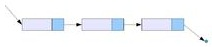
\includegraphics[width=0.4\columnwidth]{immagini/lista}
	\caption[Lista concatenata monodirezionale]{Lista concatenata monodirezionale. I campi in blu sono puntatori.}
	\label{fig:mlist}
\end{figure}
%{wrapfloat}
Con questi strumenti è possibile costruire qualcosa che somigli più di un array ad uno stack.
L'idea è di comporre una \emph{lista concatenata}, ossia una sequenza di strutture (record) con gli stessi campi che dal punto di vista logico sono ordinate tramite un dato criterio.
Esse sono generalmente ``collegate'' da puntatori (vedi la figura~\ref{fig:mlist}).
Le strutture che compongono una lista, infatti, non occupano posizioni contigue in memoria ma, nella maggior parte dei casi, sono sparpagliate.
Qui intervengono i puntatori: ogni struttura dovrà contenere un campo che punti all'elemento successivo della lista.
L'ultimo elemento avrà il campo puntatore contenente convenzionalmente il valore \lstinline!NULL! per segnare la fine della lista.
Questi accorgimenti consentono d'inserire altri record in qualsiasi posizione della lista.

Si può ora rappresentare uno stack tramite una lista concatenata.
Servirà un puntatore esterno (non contenuto in alcun record) chiamato generalmente \lstinline!*testa! che punti al nodo che si trova in alto nella pila.
Questa operazione è analoga alla dichiarazione di un contatore per segnalare il primo elemento dello stack nell'implementazione tramite gli array.
\begin{lstlisting}
struct nodo {
	int v;
	char c;
	struct nodo *next;
}
\end{lstlisting}
%	\chapter[Lezione VIII]{Lezione VIII\newline\small\emph{12/05/2010}}
	\section{Costruzione di una lista concatenata}
Come già accennato, una lista concatenata è una sequenza di oggetti, chiamati anche \emph{nodi}\index{nodo}, nella quale è definita una relazione d'ordine data dalla successione dei puntatori.
In una lista concatenata, per raggiungere l'$n$-esimo elemento bisogna percorrere tutti gli $n-1$ elementi precedenti.

Per costruire concretamente una lista concatenata c'è bisogno, oltre che degli elementi della lista, di una variabile (puntatore) che contenga l'indirizzo del primo elemento.
In generale, risulta comodo chiamare questa variabile \lstinline!*testa!, come nel codice~\ref{cod:ListaConc}.
All'inizio la lista è vuota ma \lstinline!testa! deve avere un valore legittimo: per convenzione si assegna, in questo caso, \lstinline!testa = NULL!.
Si noti che l'assegnamento \lstinline!(*pn).next = testa! equivale a \lstinline!pn->next = testa!: usare una delle due sintassi è indifferente ai fini della compilazione del programma.
\begin{lstlisting}[caption={\em Costruzione di una lista concatenata.}, label={cod:ListaConc}]
struct nodo {
	int v;
	char c;
	struct nodo *next;
} *testa, *pn;

typedef struct nodo Nodo;
testa = NULL;

/* alloco la memoria per il primo record */
pn = ( Nodo * ) malloc( sizeof( Nodo ) );
/* assegno al contatore l'indirizzo del primo record */
testa = pn;

int i = 1;
while ( i < 10 ) {
	/* alloco memoria per record successivi */
	pn = ( Nodo * ) malloc( sizeof( Nodo ) );	
	if ( pn == NULL )
		exit( EXIT_FAILURE );

	/* collego il record al precedente */
	(*pn).next = testa;
	/* modifico la testa dello stack */
	testa = pn;

	i++;
} 
\end{lstlisting}

A differenza dei vettori, i nodi della lista concatenata non sono indicizzati tramite dei numeri ma, come già accennato, tramite dei puntatori. Volendo, allora, scorrere tutti gli oggetti presenti fino all'ultimo, si scriverà un codice simile al seguente:
\begin{lstlisting}
pn = testa;
while ( pn != NULL ) {
	/* eventuali istruzioni */
	pn = pn->next;
}
\end{lstlisting}
Si tenga presente che, se la lista è vuota, il ciclo fallisce perché il test ``\lstinline!pn == NULL!'' è verificato fin dal primo elemento.

	\section{Esempi}
I codici~\ref{tab:begin},~\ref{tab:end} e~\ref{tab:middle} sono esempi di come inserire nodi in una lista concatenata rispettivamente all'inizio, alla fine ed in una posizione intermedia.
Nell'esempio~\ref{tab:middle} non sono state inserite le \MyComment{altre condizioni} perché dipendono dal criterio che si vuole usare per inserire il nodo.
	
\begin{lstlisting}[caption={\emph{Inserimento in testa}}, label={tab:begin}]
pn = ( Nodo * ) malloc( sizeof( Nodo ) );
if ( pn == NULL )
	exit( EXIT_FAILURE );

pn->next = testa;
testa = pn;
\end{lstlisting}

\begin{lstlisting}[caption={\emph{Inserimento in coda}}, label={tab:end}]
/* pi funge da contatore */
pi = testa;
/* scorro la lista finche' non finisce */
while( pi->next != NULL )
	pi = pi->next;

/* assegno all'ultimo puntatore l'indirizzo di pn (creato con malloc()) */
pi->next = pn;
/* pn e' l'ultimo, quindi il suo campo .next dev'essere NULL */
pn->next = NULL;
\end{lstlisting}

\begin{lstlisting}[caption={\emph{Inserimento intermedio}}, label={tab:middle}]
pi = testa;
while( pi->next £!\MyComment{altre condizioni}!£ )
	pi = pi->next;

pn->next=pi->next;
pi->next = pn;
\end{lstlisting}
	


%	\chapter[Lezione IX]{Lezione IX\newline\small{\emph{19/05/2011}}}
	\section{Rappresentazione dei numeri nel calcolatore}
Un sistema di rappresentazione numerica può essere \emph{posizionale} o \emph{non posizionale}.
Nel primo caso, ogni cifra assume un peso diverso a seconda della posizione in cui è scritta.
Una rappresentazione numerica è anche caratterizzata dalla \emph{base}\index{base}, che fissa il numero massimo di simboli differenti che consentiti per rappresentare le cifre; il sistema numerico occidentale è \emph{decimale posizionale}. Pertanto:
\begin{itemize}
	\item
La base stabilisce il numero di simboli differenti consentiti per rappresentare le cifre, nel nostro caso $\Set{0, \dots , 9}$.
	\item
Il fatto che sia posizionale ci garantisce che, ad esempio, $123=1\cdot 10^2+2\cdot 10^1+3\cdot 10^0 \neq 321=3\cdot 10^2+2\cdot 10^1+1\cdot 10^0$.
Ciò accade proprio perché le cifre hanno pesi differenti a seconda della loro posizione, infatti, ad esempio
\[
4814=4\cdot10^3+8\cdot10^2+1\cdot10^1+4\cdot10^0.
\]
In generale, essendo $b$ la base della rappresentazione e $c_i$ (con $i\in\{1,\dots,b\}\cap\mathbb{N}$) i rappresentatori delle cifre, dato $z\in\mathbb{N}$  si ha che, $\forall i,\dots,j\in\Set{1,\dots,b}\cap\mathbb{N}$:
\[
c_{i_z}\dots c_{j_1}=c_{i_z}10^{z-1}+\dots+c_{j_1}10^{0}=\sum_{e=1}^z c_{\{i,\dots,j\}_e}\cdot b^{e-1}.
\]
\end{itemize}

		\subsection{Esempi}
		\label{subsec:BasiExamp}
Si considerino i seguenti esempi. Le basi \emph{ottale}, \emph{esadecimale} e \emph{binaria} non sono scelte a caso; esse, infatti, sono molto usate nel campo dell'informatica. Si noti che, nel caso di rappresentazioni non decimali, è buona norma specificare la base a pedice.
\begin{description}
\item[Base] \lstinline!8!
	\begin{itemize}
		\item
Simboli: \lstinline!0, 1, 2, 3, 4, 5, 6, 7!
		\item
$523_8=5\cdot8^2+2\cdot8^1+3\cdot8^0=339_{10}$
	\end{itemize}
\item[Base] \lstinline!16!
	\begin{itemize}
		\item
Simboli: \lstinline!0, 1, 2, 3, 4, 5, 6, 7, 8, 9, A, B, C, D, E, F!
		\item
$3A2_{16}=3\cdot16^2+A\cdot16^1+2\cdot16^0=930_{10}$
	\end{itemize}
\item[Base] \lstinline!2!
	\begin{itemize}
		\item
Simboli: \lstinline!0, 1!
		\item
$101101_{2}=1\cdot2^5+0\cdot2^4+1\cdot2^3+1\cdot2^2+0\cdot2^1+1\cdot2^0=45_{10}$
	\end{itemize}
\end{description}

		\subsection{Passare in base \lstinline!2!}
Per passare da una base, ad esempio \num{10}, in base \num{2}, si può utilizzare il seguente metodo, che è il procedimento inverso di quelli mostrati nel paragrafo~\ref{subsec:BasiExamp}.\footnote{Si noti che per passare ad una base $b$ qualsiasi, si può usare lo stesso procedimento sostituendo a \num{2} il numero $b$.}

S'individua la massima potenza di \num{2} che non supera il numero $m$ di partenza, sia essa $n$.
Se $2^n-m\eqqcolon z_1=0$, il numero binario si ottiene ponendo $1$ nella posizione $n+1$ e zero nelle posizioni da $n$ in giù.
In caso contrario, se $z_1\neq0$, si trova la massima potenza di \num{2} che non superi $z_1$ e si ripete il procedimento finché non s'individua un indice $i\in\{1,\dots,\log_2n+1\}\cap\mathbb{N} \mid z_{i}=0$.
Ad esempio:
\[
45_{10}=\underbrace{32+8+4+1}_{2^5+2^3+2^2+2^0}=101101_{2}
\]


Tale algoritmo, tuttavia, è piuttosto scomodo da stendere come programma e risulterebbe onerebbe per il calcolatore. Si può allora pensare ad un altro procedimento: un'alternativa è la seguente.
Si divide il numero $m$ di partenza per \num{2}.
Il resto $r_1$ di tale operazione è la prima cifra (quella con il peso minore) del numero binario.
Si divide ora il quoziente $q_1$ (intero) per \num{2}.
Come prima,  il resto è la seconda cifra del numero.
Il procedimento termina quando s'individua un indice $i\in\{1,\dots,\log_2n+1\}\cap\mathbb{N} \mid q_{i}=0$.
Ecco un esempio:
\[
\dfrac{45}{2}=22+\mathbf{1};\ 
\dfrac{22}{2}=11+\mathbf{0};\ 
\dfrac{11}{2}=5+\mathbf{1};\ 
\dfrac{5}{2}=2+\mathbf{1};\ 
\dfrac{2}{2}=1+\mathbf{0};\ 
\dfrac{1}{2}=0+\mathbf{1}.\ 
\]
Chiaramente, tale algoritmo è molto più semplice da tradurre in un programma in \lang{C} e risulta molto più efficiente del precedente.

	\subsection{bit e byte}
L'unità di misura della memoria in un calcolatore è il \si{\bit}\index{bit} (\emph{Binary Digit}, cioè \emph{Cifra Binaria}).
Il suo primo multiplo è il \si{byte}\index{byte} (dove si ha che $\SI{1}{\byte} = \SI{8}{\bit}$), corrispondente a quello che veniva chiamato ``quadretto'' nel paragrafo~\ref{sec:mem} a pagina~\pageref{sec:mem}.
Con un \si{byte} si ottengono $2^8=256$ combinazioni differenti, quindi, in teoria, \num{256} caratteri diversi.
In realtà, la combinazione \lstinline!00000000! non viene considerata un carattere pertanto le rappresentazioni effettivamente ammesse sono $2^8-1=255$: i caratteri \acs{ascii}.
In generale, $n\,\si{\bit}$ danno $2^n$ combinazioni e $2^n-1$ rappresentazioni di caratteri.

Nel calcolatore normalmente una variabile di tipo \lstinline!int! occupa \SI{4}{\byte}, ossia $(2^8)^4=2^{8\cdot4}=\num{4294967296}$ combinazioni.
Se gli interi fossero soltanto non negativi, dunque, il più grande numero rappresentabile sarebbe \num{4294967295}.
Tuttavia, variabili di tipo \lstinline!int! possono assumere valori sia positivi che negativi.
Si stabilisce, allora, di destinare il primo \si{bit} di un intero al segno del numero: per convenzione, si associa \num{0} al segno negativo e  il valore \num{1} al segno positivo.

Assumiamo, per semplicità, che un intero sia rappresentato da \SI{4}{\bit}.
Allora, le rappresentazioni \lstinline!1000! e \lstinline!0000! corrispondono (infatti $\num[parse-numbers=false]{-0_{10}}=\num[parse-numbers=false]{+0_{10}}$).
Avendo destinato un \si{bit} al segno, restano soltanto $2^{\textup{num.~di \si{\bit}}}-1$ rappresentazioni differenti, \num{255} nella fattispecie.
Per ovviare a questo problema, si ricorre al metodo del \emph{complemento a due}.

	\subsection{Complemento a due}

\begin{figure}
	\centering
	\begin{tikzpicture}[scale=0.8]
\foreach \ang/\dl/\bl in {90/0/0000,67.5/1/0001, 45/2/0010,
22.5/3/0011,0/4/0100,-22.5/5/0101,-45/6/0110,-67.5/7/0111,
-90/-8/1000,-112.5/-7/1001, -135/-6/1010,-157.5/-5/1011,
-180/-4/1100,-202.5/-3/1101,-225/-2/1110,-247.5/-1/1111} {
	\draw [black] node [circle,draw,minimum size=1cm,label=below:{\color{blue}$\mathtt{\bl}$},top color=gray] at (\ang:5) {$\dl$};
}
	\end{tikzpicture}
	\caption[Complemento a due]{Rappresentazione del complemento a due con numeri di \SI{4}{\bit}.}
	\label{fig:2comp}
\end{figure}

S'immagini di sistemare sul bordo di un anello tutte le combinazioni date da un certo numero di \si{\bit} (se ne considerino sempre quattro, per comodità) come in figura \ref{fig:2comp}.
Ora, s'interpretino nel modo usuale i numeri che hanno come prima cifra (partendo da sinistra) \num{0}.
Cominciando da \lstinline!0000! e spostandosi in senso orario, dunque, si hanno numeri interi crescenti fino al numero \lstinline!1000!.
Si stabilisce, altresì, di assegnare ai numeri che hanno \lstinline!1! come prima cifra valori progressivamente più piccoli partendo da $-1$ (\lstinline!1111!) e proseguendo in senso antiorario.

Si ha che, ad esempio, considerando la somma delle rappresentazioni binarie dei numeri \num[parse-numbers=false]{-6_{10}} e \num[parse-numbers=false]{-2_{10}}:
\[
	\begin{array}{r l}
\mathtt{1010}	&+	\\
\mathtt{1110}	&=	\\
		\midrule
\mathtt{11000}
	\end{array}
\]
Siccome un numero è composto di \SI{4}{\bit}, il calcolatore memorizzerà solo \lstinline!1000! che corrisponde a \num[parse-numbers=false]{-8_{10}}.
Si prendano altri casi:
\[
\mathtt{
3+(-5)=
	\begin{array}{r l}
\mathtt{0011}	&+	\\
\mathtt{1011}	&=	\\
		\midrule
\mathtt{1110}
	\end{array}
\quad \rightarrow-2_{10}
}
\]
Si noti che non c'è stato bisogno d'introdurre l'operazione di differenza.
Una volta definita la somma, non serve altro.
Ancora:
\[
\mathtt{
5+(-3)=
	\begin{array}{r l}
\mathtt{0101}	&+	\\
\mathtt{1011}	&=	\\
		\midrule
\mathtt{10010}
	\end{array}
\quad \rightarrow2_{10}
}
\]
Tuttavia:
\[
\mathtt{
3+6=
	\begin{array}{r l}
\mathtt{0111}	&+	\\
\mathtt{0110}	&=	\\
		\midrule
\mathtt{1101}
	\end{array}
\quad \rightarrow-3_{10}
}
\]
Ciò accade perché il numero \num{13} non può essere rappresentato con \SI{4}{\bit}.
Infatti, tale metodo è corretto solo per numeri $n\in\{-8,-7,\dots,7\}$ (o, in generale, essendo $m$ il numero di \si{\bit}, $-2^{m-1}-1\le n \le 2^{m-1}-1$).
Questo è un errore comunemente chiamato \emph{overflow}\index{overflow} o \emph{tracimazione}\index{tracimazione}.

		\subsection{Virgola mobile}
Finora, è stata trattata soltanto la rappresentazione di un intero ($n\in\mathbb{Z}$) in un calcolatore.
Si considerino ora dei numeri $q\in\mathbb{Q}$.
Affinché essi siano rappresentati in memoria si deve introdurre il concetto di \emph{virgola mobile} (o, in inglese, \emph{floating point}).
Siano dati i seguenti numeri decimali:
\[
	\begin{split}
&\num[parse-numbers=false]{2,718_{10}}=2\cdot10^0+7\cdot10^{-1}+1\cdot10^{-2}+8\cdot10^{-3};	\\
&101,01_2=1\cdot2^2+0\cdot2^1+1\cdot2^0+0\cdot2^{-1}+1\cdot2^{-2}.
	\end{split}
\]
Nella sua rappresentazione più semplificata, un numero in virgola mobile è composto da:
\begin{itemize}
	\item
Mantissa;
	\item
Esponente;
	\item
Base.
\end{itemize}
Bisogna tenere conto che, come in precedenza, anche qui il primo \si{bit} viene riservato al il segno.
Le cifre significative sono rappresentate dalla \emph{mantissa}\index{mantissa}.
Si ha che:
\[
2,718_{10}=\underbrace{2718}_{\textup{Mantissa}}\cdot{\underbrace{10}_{\textup{Base}}}^{(-3)\ \rightarrow\textup{Esponente}}
\]
Tra le infinite rappresentazioni in virgola mobile, si stabilisce una forma ``canonica''.
Essa prevede che:
\begin{itemize}
	\item
Siano $m, b$ rispettivamente la mantissa e la base, allora si deve avere che: $0<m<b$;
	\item
L'esponente della base dev'essere il più piccolo possibile.
\end{itemize}

In memoria, un numero in virgola mobile è rappresentato secondo il seguente schema:
\begin{center}
\textit{
	\begin{tabular}{|c|c|c|}
		\toprule
segno	&esponente	&mantissa	\\
		\bottomrule
	\end{tabular}
}
\end{center}


Se un numero in virgola mobile occupa \SI{32}{bit}, a segno, esponente e mantissa vengono assegnati rispettivamente \SI{1}{\bit}, \SIrange[range-phrase={ e }]{8}{23}{\bit}.
Se invece occupa \SI{64}{\bit} sono assegnati \SI{1}{\bit} per il segno, \SI{11}{\bit} per la mantissa e \SI{52}{\bit} per l'esponente.

Si tenga presente che nelle operazioni algebriche, il calcolatore interpreta la mantissa $m$ come se fosse $m+1$.

	\section{Strutture di controllo}
Durante \marginpar{Il ciclo \lstinline!for()!} tutta la trattazione è stata introdotta una sola notazione per le iterazioni: il ciclo \lstinline!while()! (vedi il paragrafo~\ref{sec:it} a pagina~\pageref{sec:it}).
Esiste, tuttavia, un altra sintassi che risulta in parecchie occasioni più conveniente: il ciclo \lstinline!for()!.

		\subsection{Ancora sulle iterazioni}

Il riquadro~\ref{cod:for()} mostra un ciclo \lstinline!while()! e il suo equivalente ciclo \lstinline!for()!.
Il secondo prevede una sintassi molto più contenuta e, nella maggior parte dei casi, rende il codice molto più leggibile.



La sintassi del ciclo \lstinline!for()! è:
\begin{lstlisting}
for( £!\MyComment{prima istruzione}!£; £!\MyComment{test}!£; £!\MyComment{ultima istruzione}!£ ) {
	£!\MyComment{corpo}!£
}
\end{lstlisting}

Il compilatore esegue la \MyComment{prima istruzione}, che in generale è un assegnamento, \emph{una sola volta} all'inizio del ciclo e poi:
\begin{enumerate}
	\item\label{for:test}
Controlla il risultato del \MyComment{test}:
	\begin{enumerate}
		\item\label{test:true}
Se è \lstinline!true!, esegue il corpo del ciclo;
		\item\label{test:false}
 Se è \lstinline!false! lo interrompe.
\end{enumerate}
	\item
Nel caso~\ref{test:true}, esegue il \MyComment{corpo} e infine l'\MyComment{ultima istruzione};
	\item
Riparte da~\ref{for:test} e continua finché non si verifica~\ref{test:false}.
\end{enumerate}

\begin{code}
\centering
	\caption{Confronto tra il ciclo \lstinline!while()! ed il ciclo \lstinline!for()!.}
	\label{cod:for()}
\begin{minipage}{0.45\columnwidth}
	\begin{lstlisting}
#define N 10

int i = 0;
while ( i < N ) {
	s = s + p[i];
	i ++;
}
	\end{lstlisting}
\end{minipage}	\hfill
\begin{minipage}{0.45\columnwidth}
	\begin{lstlisting}
#define N 10

int i;
for ( i = 0; i < N; i ++ ) {
	s = s + p[i];
}
	\end{lstlisting}
\end{minipage}
\end{code}
%	\chapter[Lezione X]{Lezione X\newline\small{\emph{26/05/2011}}}
	\section{Breve storia dell'informatica}
L'\emph{informatica} è una disciplina che si fonda su due pilastri fondamentali:
\begin{description}
	\item[Teoria della computazione;] (Turing, Church, Post nel 1936) che si occupa di studiare il concetto di ""algoritmo'' e tutto ciò che ne consegue;
	\item[Teoria dell'informazione;] (Shannon nel 1949) che nasce essenzialmente dal problema di trasportare messaggi da un luogo ad un altro nel modo più sicuro ed efficiente possibile.
\end{description}

		\subsection{Teoria della computazione}
La \emph{teoria della computazione} nasce dalla domanda: cosa è possibile calcolare meccanicamente?

Parte della teoria si spende nello specificare innanzitutto il significato della parola ""meccanicamente''. Data la generalità di questa trattazione, si può assumere che significhi ""seguendo delle istruzioni fisse''.

		\subsection{La macchina di Turing}
		\label{subsec:mturing}
Negli anni '30 esistevano già le calcolatrici, ma la tecnologia non rendeva ancora disponibile alcunché di più avanzato. C'erano,\marginpar{Computer e contabili} tuttavia i \emph{computer} che, in lingua inglese, erano i contabili. Alan Mathison Turing (vedi il paragrafo~\vref{subsec:turing}) s'ispirò proprio al modo di lavorare del contabile per mettere a punto la sua idea si calcolatore. Il contabile, infatti, è chiamato ad eseguire dei calcoli applicando formule date a priori, una matita ed un foglio. Non ha bisogno di usare la creatività o l'inventiva. Svolge solo dei calcoli e, di tanto in tanto, si serve del foglio e della matita per appuntare dei risultati intermedi. Il contabile ha inoltre a disposizione una quantità finita di segni differenti da poter usare. Riesce a riconoscere ed interpretare solo un numero finito di simboli. Anche il foglio (a quadretti) di cui dispone ha una dimensione limitata. Inoltre, in ogni quadretto c'è lo spazio per uno ed un solo simbolo. Egli può anche trovarsi in un numero finito di quelli che Turing denominò ""stati mentali'', ossia delle ""condizioni interne'' che lo fanno reagire in modo diverso a degli stimoli provenienti dall'esterno.

\begin{wrapfloat}{figure}{i}{0pt}
	\centering
	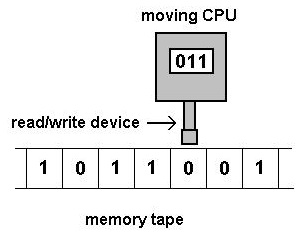
\includegraphics[width=0.5\columnwidth]{immagini/turing}
	\caption{Macchina di Turing.}
	\label{fig:tm}
\end{wrapfloat}
Partendo \marginpar{Macchina di Turing} da quanto detto finora, Turing immaginò la cosiddetta \emph{Macchina di Turing} (figura~\vref{fig:tm}). Molto schematicamente, si tratta di una scatola che può trovarsi in un numero finito di stati interni differenti. Dalla scatola si protende un braccio che dà su un nastro scorrevole. Quest'ultimo contiene dei numeri, dei caratteri alfanumerici o niente. Tale nastro può essere allungato indefinitamente, pur restando di lunghezza finita. Il braccio è in grado sia di leggere dal nastro che di scrivervi sopra. Il cuore dell'apparecchio è la \emph{tabella delle istruzioni}.

Sia $S$ l'insieme degli stati interni assumibili dalla macchina e $A$ l'insieme dei simboli che essa riesce a riconoscere:
\[
\left[
	\begin{aligned}
S &= \{ \sigma_1, \dots, \sigma_n \}; \\
A &= \{ \alpha_1, \dots, \alpha_m \};
	\end{aligned}
\right.
\text{ con } m,n \in \mathbb{N}.
\]
Le istruzioni della macchina, allora, hanno la forma:
\begin{quote}
""se (il tuo stato è $\sigma_i$) e se (leggi $\alpha_e$ nella casella); allora (cambia stato in $\sigma_r$, sposta la testina a destra e scrivi\dots)''
\end{quote}
Ad un certo punto, la macchina troverà un'istruzione di \lstinline!stop! e si fermerà. Allora si possono fissare gli insiemi dell'alfabeto $A$ e degli stati interni $S$ (delle istruzioni):
\begin{itemize}
	\item
\emph{Alfabeto}: codice binario;
	\item
\emph{Istruzioni:}
		\begin{itemize}
			\item
Se (la testina legge un numero) $\rightarrow$ (va a destra);
			\item
Se (la testina legge una casella vuota) $\rightarrow$ (scrive nella prima casella vuota ""$0$'').
		\end{itemize}
\end{itemize}
In pratica, tale funzione aggiunge uno \lstinline!0! ad un numero binario, che corrisponde a raddoppiarlo.

		\subsection{Problemi insolubili}
		\label{subsec:ins}
Con questo tipo di macchine è possibile calcolare funzioni $f:\mathbb{N}\mapsto\mathbb{N}$ come, ad esempio, $f(n)=2n;\ f(n)=\sqrt{n}$ (purché ci si accontenti della sola parte intera)$; f(n)=n^2+n+1 \dots$ Esistono, tuttavia, delle funzioni che non possono essere calcolate con una macchina di Turing dal momento che non esiste un processo meccanico (algoritmo) che porti alla loro soluzione\footnote{Questo si può dimostrare provando che l'insieme funzioni aritmetiche calcolabili è un sottoinsieme di quello delle funzioni aritmetiche. Dal momento che una funzione aritmetica è calcolabile se e solo se esiste un algoritmo che la calcola \parencite{fp:comp}, segue la tesi.}.

Non \marginpar{Polinomio di grado qualsiasi} esiste un algoritmo che, dato un polinomio a coefficienti interi di grado non fissato a priori, sia in grado di stabilire se esistano o meno delle radici intere. Tale risultato è ottenibile solo conoscendo in anticipo il grado del polinomio.

Un'altra \marginpar{Problema dell'arresto} questione non risolubile è il cosiddetto \emph{problema dell'arresto}. Si consideri un codice del tipo:
\begin{lstlisting}
i = 1;
while( i > 0 )
	i++;
\end{lstlisting}
Esso genera un ciclo teoricamente infinito. Una volta avviato non può arrestarsi, tranne che per cause esterne\footnote{Vedi: ""black out'', oppure ""utente incavolato che sfascia il computer perché il suo programmino non funziona''\dots}. Dopo aver compilato il programma, non c'è alcuna possibilità d'individuare un errore di questo tipo durante l'esecuzione. Non si può dimostrare di aver scritto un ciclo infinito (anche se ad un certo punto, cominciano a sorgere forti sospetti\dots). Si potrebbe pensare, allora, di scrivere un programma che verifichi il codice di un altro dal punto di vista logico. Lo stesso Turing dimostrò che un siffatto programma non può essere steso.

		\subsection{La macchina universale}
Presa una macchina di Turing tale che:
\[
	\begin{aligned}	
	&\left[
		\begin{aligned}
&S=\{\sigma_1, \sigma_2, \sigma_3\}; \\
&A=\{1, 0\};	\\
		\end{aligned}
	\right .	\\
&\sigma_1, 0 \rightarrow 1, \sigma_2, \text{ destra};	\\
&\vdots
	\end{aligned}
\]
Si possono tradurre gli stati interni del computer usando il suo alfabeto (il codice binario). Nello specifico, ci sono tre (11) stati , e due (10) simboli. Adottando le convenzioni delle tabelle~\vref{tab:istr} e~\vref{tab:stat} è possibile tradurre le istruzioni in linguaggio binario.
\begin{table}
	\centering
\subfloat[][{\em Rappresentazione binaria delle istruzioni.}\label{tab:istr}]{
	\begin{tabular}{l c}
		\toprule
\emph{Istruzione}			&\emph{Numero}	\\
		\midrule
Sposta la testina a destra		&\lstinline!0!	\\
Sposta la testina a sinistra		&\lstinline!1!	\\
		\bottomrule
	\end{tabular}
}\quad
\subfloat[][{\em Rappresentazione binaria degli stati interni.}\label{tab:stat}]{%}
	\begin{tabular}{l c}
		\toprule
\emph{Stato}			&\emph{Numero}	\\
		\midrule
$\sigma_1$				&\lstinline!01!	\\
$\sigma_2$				&\lstinline!10!	\\
$\sigma_3$				&\lstinline!11!	\\
		\bottomrule
	\end{tabular}
}
	\caption[Macchina di Turing]{Convenzioni binarie per la macchina di Turing}
\end{table}
Si ha che:
\[
	\begin{aligned}	
	&\left[
		\begin{aligned}
&\mathtt{01\ 10\ 11} 		\\
&\mathtt{1\ 0} 			\\
		\end{aligned}
	\right .	\\
&\mathtt{1\_0\_1\_10\_0}	\\
&\vdots
	\end{aligned}
\]
Il problema di distinguere i numeri da elaborare dalle istruzioni è facilmente risolvibile.

Ora, una macchina di Turing può essere descritta con un numero. Si consideri, allora, una macchina $U$ che riesca a riconoscere parti di codice di altre macchine. Si hanno due macchine $E$ e $D$ tali che:
\[
\left\{
	\begin{aligned}
&E:\,f(x)=2 		\\
&D:\,f(x)=x^2-1
	\end{aligned}
\right.
\]
Se alla macchina $E$ corrisponde il codice \lstinline!1_0_11_0_1!, allora la macchina $U$ riesce ad interpretarlo come istruzione ed applicarlo su un numero $x$ (\lstinline!101!, ad esempio). Tale macchina $U$ è una cosiddetta \emph{macchina Universale}. In questo modo non si deve progettare un apparecchio specifico per ogni algoritmo da eseguire, ma ne basta uno solo. 

Da \marginpar{La tesi di Church-Turing} quanto detto finora, discende la \emph{tesi\footnote{Si noti che \emph{non} è un teorema perché discende direttamente da tutta la teoria ""costruita'' da Turing.} di Church-Turing}:
\begin{quotation}
"<Le funzioni calcolabili dalla macchina di Turing sono \emph{tutte e sole} quelle calcolabili meccanicamente.">
\end{quotation}
Gli studi di John von Neumann negli anni '40 (vedi il paragrafo~\vref{sec:neu}) si basavano proprio sulle osservazioni di Turing.

	\section{Algoritmo di Dijkstra per i cammini minimi}
Un \emph{grafo} (vedi il paragrafo~\vref{subsec:grafo}) è un oggetto composto di vertici (o \emph{nodi}) e lati (o \emph{archi}). Un arco ""unisce'' due nodi. Siano V ed E rispettivamente gli insiemi dei vertici e lati, allora:
\[
\begin{split}
&V=\{(x_1,y_1),\dots,(x_n,y_n)\} \\
&E\subseteq V\times V
\end{split}
\]
Se si associa ad ogni lato $e_{i}\in E$ un numero $z_i\in\mathbb{R^{+}}$, è naturale interpretare $z_i$ come la distanza che intercorre tra i due nodi collegati dall'arco $e_i$.Dato un grafo, è lecito chiedersi quale sia il \emph{cammino minimo} (o cammino di minimo costo) tra due suoi punti qualsiasi. Per rispondere a tale domanda, ci si serve dell'{\em algoritmo di Dijkstra}.

Si vuole calcolare il cammino più breve che collega il vertice A della figura~\ref{fig:dij} con tutti gli altri. Per fare ciò è conveniente registrare tutti i possibili percorsi (con le rispettive distanze) in una tabella come la~\ref{tab:dij}. Si trovano i nodi immediatamente vicini ad $A$. Si ha che $\overline{AB}=5$ e $\overline{AE}=1$. Per ora, queste sono le distanze minime. Partendo ora da B, si ha che $\overline{AC}=\overline{AB}+\overline{BC}=8$ e $\overline{AD}=\overline{AB}+\overline{BC}=6$. Entrambi questi percorsi individuano, al momento, dei cammini minimi. Ripetendo l'operazione per tutti i vertici del grafo, si ottiene tabulata la distanza minima tra $A$ e qualsiasi altro nodo (ma anche tra due vertici qualsiasi $v_1,v_2\in\{A, B, C, D, E, F, G\}$).
\begin{figure}
	\centering
	\subfloat[][{\em Rappresentazione del grafo.}\label{fig:dij}]{
%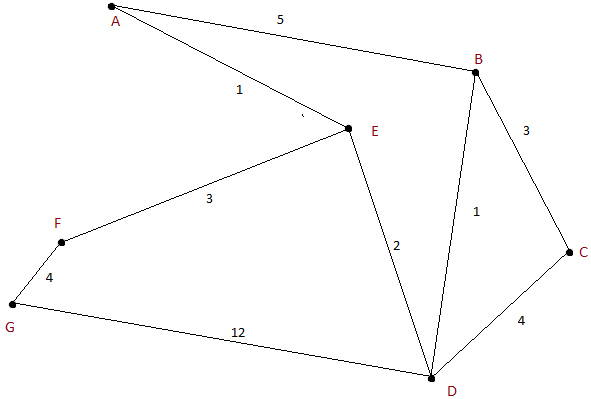
\includegraphics[width=\columnwidth]{immagini/dijkstra}
\begin{tikzpicture}
	\coordinate (A) at (-2,6);
	\coordinate (B) at (2,5);
	\coordinate (C) at (4,2);
	\coordinate (D) at (3,0);
	\coordinate (E) at (1,4);
	\coordinate (F) at (-1,3);
	\coordinate (G) at (-2.5,0.5);

	\foreach \a/\b/\d in {A/B/5, B/C/3, C/D/4, D/G/12, G/F/4, F/E/3, A/E/1, D/E/2, D/B/1}
		\draw [line width=0.5pt, color=blue] (\a) -- (\b) node [blue, sloped,midway,above] {$\d$};

	\foreach \n in {A,B,C,D,E,F,G} 
		\draw [] node [circle,draw,minimum size=1cm,top color=gray] at (\n) {\color{black}{\n}};

\end{tikzpicture}
}	\\
	\subfloat[][{\em La tabella contiene alcune distanze partendo dal vertice A. Il cammino minimo è evidenziato.}\label{tab:dij}]{
\begin{tabular}{l l l}
	\toprule
\emph{Vertice}	&\emph{Distanza}		&\emph{Percorso}		\\
	\midrule
$A$ 			&0			& /					\\
$B$ 			&\textbf{5}		&$\mathbf{AB}$			\\
$C$ 			&8; \textbf{7}	&$ABC; \mathbf{AEDC}$		\\
%$D$ 		&12; 6; \textbf{3}	&$ABCD; ABD;\mathbf{AED}$	\\
%$E$ 		&\textbf{1}		&$\mathbf{AE}$			\\
\vdots 		&\vdots 		& \vdots 				\\
	\bottomrule
\end{tabular}
}\quad
	\subfloat[][\emph{Matrice $n\times n$. Si noti che sulla diagonale ci siano solo valori nulli.}\label{tab:mat}]{
	\begin{tabular}{>$c<$ | >$c<$ >$c<$ >$c<$ >$c<$}
		&v_1		&v_2		&\dots 	&v_N 		\\
		\midrule
v_1		&0		&4.5		&\dots 	&0		\\
v_2		&3		&0		&\dots 	&5.7		\\
\vdots 	&\vdots 	&\vdots 	&\ddots 	&\vdots 	\\
v_ N		&8.9		&0		&\dots 	&0		\\
	\end{tabular}
}\\
	\subfloat[][{\em Grafo con rappresentazione per lista adiacenze e rappresentazione matriciale.}\label{fig:adi}]{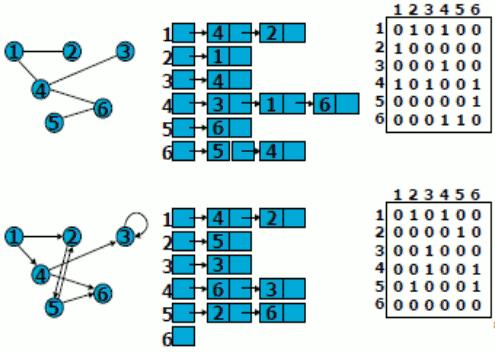
\includegraphics[width=\columnwidth]{immagini/lista_adiacenze}}
	\caption{Algoritmo di Dijkstra}
	
\end{figure}

Per \marginpar{Rappresentazioni in C} tradurre tale algoritmo in linguaggio C, c'è innanzitutto bisogno di trovare una rappresentazione per il grafo. Vi sono diverse soluzioni:
\begin{itemize}
	\item
Si rappresentano i vertici con degli interi e il lati con un record che contenga informazioni sui nodi che collega e la loro distanza;
	\item
Si usa una matrice.

Avendo dei vertici $v_{i\in\{1,\dots,N\}}\in V$, si dichiara una matrice $N\times N$ come la tabella~\vref{tab:mat} e si stabilisce che:
	\begin{itemize}
		\item
Se tra due vertici c'è un lato, si scrive nella casella corrispondente il valore $1$ (o la distanza $z\in\mathbb{R^{+}}$);
		\item
Se tra due vertici non c'è un lato, si scrive nella casella corrispondente il valore $0$.
	\end{itemize}
Si noti, che avendo dichiarato una matrice \lstinline!float m[N][N];! si ha che \lstinline!m[e][j] == 0! $\forall e,j\in\{1,\dots,N\}\mid e=j$ se non esistono archi che colleghino un punto con se stesso, come in figura~\ref{fig:dij}. Con questa rappresentazione, il costo computazionale dell'algoritmo di Dijkstra (siccome sulla diagonale ci sono solo valori nulli) è $N^2-N\thicksim N^2$ per $N\to+\infty$. Pertanto, la rappresentazione matriciale risulta piuttosto scomoda se il grafo è sparso, cioè se ci sono pochi archi.
	\item
Ci si serve di una \emph{lista adiacenze}.

Essa, come mostra la figura~\vref{fig:adi}, consiste in più serie di record ognuna delle quali si riferisce ad un nodo di partenza differente. Ogni struttura contiene un campo che tenga traccia del nome del nodo collegato e un campo puntatore alla struttura successiva. Nel campo puntatore dell'ultimo record, ormai è inutile dirlo, si pone il valore \lstinline!NULL!.

Tale rappresentazione risulta piuttosto ridondante per grafi non orientati perché si usano due record per ogni arco, ma diventa più efficiente nel caso di grafi orientati. Si noti che, volendo aggiungere il ""peso'' di ogni lato, si dovrebbe aggiungere ad ogni record un campo dedicato.
\end{itemize}
%	\chapter[Lezione XI]{Lezione XI\newline\small{\emph{06/03/2011}}}

	\section{Lezione pre-esame}

Per un manuale on-line affidabile sulla sintassi in linguaggio \lang{C}, è possibile fare riferimento a~\cite{wiki:en}. % \textsf{C syntax} su \href{http://en.wikipedia.org/wiki/Main_Page}{Wikipedia} (in inglese).

		\subsection{Modello (o struttura) dei dati}
Le strutture dati studiate finora sono le seguenti (tranne le ultime due, cui s'accennerà in seguito):
\begin{itemize}[noitemsep]
	\item
Array o vettori, matrici (vedi il paragrafo~\ref{subsec:array} a pagina~\pageref{subsec:array});
	\item
Grafi (vedi il paragrafo~\ref{subsec:grafo} a pagina~\pageref{sucsec:grafo});
	\item
Record o strutture (vedi il paragrafo~\ref{subsec:record} a pagina~\pageref{subsec:record});
	\item
Stack (vedi il paragrafo~\ref{subsec:stack} a pagina~\pageref{subsec:stack});
	\item
Liste concatenate (vedi il paragrafo~\ref{subsec:liste} a pagina~\pageref{subsec:liste});
	\item
Code (vedi il paragrafo~\ref{subsec:coda});
	\item
Alberi (vedi il paragrafo~\ref{subsec:albero}).
\end{itemize}
Ciascuno di questi modelli si caratterizza per le operazioni che permette di compiere.
Nelle liste concatenate trattate nel  paragrafo~\ref{subsec:stack}, ad esempio, sono definiti l'inserimento (con la funzione \lstinline!push()!) e la cancellazione di elementi (tramite la funzione \lstinline!pop()!).


In ogni caso, una struttura dati non è troppo vincolante: è possibile creare una lista concatenata usando una matrice, ad esempio.
Dichiarando una matrice di $n$ righe, si possono destinare le prime $n-1$ al ``carico utile'' e l'$n$-esima a puntare al nodo successivo, come campo \lstinline!*next!.
Così facendo, è come se una colonna di una matrice rappresentasse un nodo.
Tuttavia, poiché le matrici sono indicizzate tramite interi $z$ progressivi, basterà un intero per identificare l'indirizzo del nodo successivo.
Come ultimo accorgimento, basta stabilire che il nodo di coda contenga nella sua $n$-esima riga un intero negativo ad indicare la fine della lista.
Ad ogni modo, servirà comunque una variabile ausiliaria (analogamente al puntatore \lstinline!*testa!) di tipo \lstinline!int! che indichi qual è il primo nodo.


\begin{figure}
	\centering
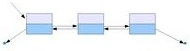
\includegraphics[width=0.45\columnwidth]{immagini/lista_bidirezionale}
	\caption[Lista concatenata bidirezionale]{Lista concatenata bidirezionale: i campi in blu sono puntatori.}
	\label{fig:blist}
\end{figure}
Per l'esame, potrebbe essere necessario apportare delle modifiche ad una struttura dati esistente, come creare una lista concatenata bidirezionale (vedi la figura~\ref{fig:blist}).
Tale struttura ha bisogno di due campi puntatore (\lstinline!*prev! e \lstinline!*next!) e può essere percorsa in entrambi i versi.
Oppure, si potrebbero dover dichiarare più campi puntatori all'interno di un record per ordinare la lista in base a criteri differenti.

	\section{Strutture dati}

		\subsection{Coda}
		\label{subsec:coda}

\begin{figure}
	\centering
%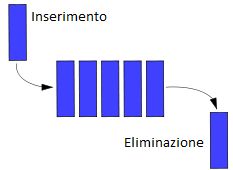
\includegraphics[width=0.45\columnwidth]{immagini/coda}
\begin{tikzpicture}[
	scale = 1.5,
	x={(1 cm,0 cm)},
	z={(-.35cm,-.22cm)},
	y={(0cm,1cm)}
]
\tikzset{zxplane/.style={canvas is zx plane at y=#1,very thin}}
\tikzset{yxplane/.style={canvas is yx plane at z=#1,very thin}}

%\begin{scope}[]
%			\node[rotate = 90] () at (-1.3,.5) {stack};
		\begin{scope}[canvas is yx plane at z=0]
			\draw [->, shorten >=4pt] (-1.3,-1.1) arc (180:90:1) node [at start,below] {\algo{inserimento}};
%			\draw [<-,shorten >=4pt] (2.5,1.1) arc (0:-90:1) node [at start,above] {\algo{push}};
		\end{scope}

		\begin{scope}[zxplane=-.3]
			\draw[fill=black!50!blue, opacity=.3] (1,0) arc (0:360:1) ;
		\end{scope}



	\foreach \x in {0,1,...,10} {
		\begin{scope}[zxplane=\x/10]
			\draw[fill=black!50, opacity=.3] (1,0) arc (0:360:1) ;
		\end{scope}
	}
		\begin{scope}[zxplane=1.3]
			\draw[fill=black!50!red, opacity=.3] (1,0) arc (0:360:1) ;
		\end{scope}

		\begin{scope}[canvas is yx plane at z=0]
%			\draw [->, shorten >=4pt] (2.3,-1.1) arc (0:90:1) node [at start,above] {\algo{pop}};
			\draw [<-,shorten >=4pt] (2.3,1.1) arc (0:-90:1) node [at start,above] {\algo{eliminazione}};
		\end{scope}
%\end{scope}

\end{tikzpicture}
	\caption[Coda]{Rappresentazione grafica di una coda.}
	\label{fig:coda}
\end{figure}
La \emph{coda}\index{coda}, mostrata in figura~\ref{fig:coda}, è una struttura dinamica lineare: gli elementi, cioè, sono ordinati.
A differenza di uno stack, tuttavia, essi seguono una disciplina del tipo \ac{fifo}.
Un nuovo oggetto inserito si colloca in fondo alla coda, mentre per estrarne uno lo si preleva dalla testa.

Risulta ora evidente l'analogia di tale struttura con una fila (o coda) reale che si fa per usufruire di un servizio ad uno sportello, da cui peraltro prende il nome.
\begin{table}
	\centering
	\caption[Costo computazionale]{La tabella mostra il costo computazionale di uno stack, una coda ed una coda con un puntatore all'ultimo elemento con $n$ elementi.}
	\label{tab:co-st}
	\begin{tabular}{l  S[parse-numbers=false] S}
		\toprule
Struttura		&{Inserimento}	&{Eliminazione}	\\
		\midrule
	Stack			&1				&1				\\
	Coda			&n				&1			\\
	Coda (puntatore)	&1				&1				\\
\bottomrule
	\end{tabular}
\end{table}
Differenze tra coda e stack si riscontrano anche nel costo computazionale, ossia sul numero di ``calcoli'' che l'esecutore deve compiere per effettuare un'operazione sulla struttura, come mostra la tabella~\ref{tab:co-st}.
Per eliminare un elemento, partendo da \lstinline!*testa!, il computer deve percorrere tutta la coda finché non giunge all'ultimo.
Per ridurre il costo computazionale della coda, è possibile introdurre un puntatore al nodo finale in modo tale che l'eliminazione comporti un solo passaggio, al pari dell'inserimento.

		\subsection{Albero}
		\label{subsec:albero}
Un \emph{albero} è un modello dei dati che sfrutta una struttura gerarchica.
Esistono diverse implementazioni di albero; in prima battuta si può considerare una rappresentazione che preveda due campi puntatore per ogni struttura, siano essi \lstinline!*min! e \lstinline!*max!.

\begin{figure}
	\centering
\subfloat[][Rapresentazione grafica di un \acs{bst}.\label{fig:albero_BST_nr}]{
	\begin{tikzpicture}[
	every node/.style = {
		circle,
		opacity=.4,
		inner sep=2pt,
%		minimum width={ width("50") + 3 pt},
%		text width={width("Magnetometer")},
%		align=center,
		text opacity=1
	},
%level distance=30pt
]
\tikzstyle{level 1}=[sibling distance = 23mm]
\tikzstyle{level 2}=[sibling distance = 15mm]
\tikzstyle{level 3}=[sibling distance = 12mm]

	\node [ball color = red] { $50$ }
		child {
			node [ball color=purple] {$17$}
				child{
					node [ball color=blue] {$12$}
						child{
							node [ball color=green] {$10$}
						}
						child{
							node [ball color=green] {$14$}
						}
				}
				child{
					node [ball color=blue] {$23$}
						child{
							node [ball color=green] {$19$}
						}
				}
		}
		child{
			node [ball color=purple] {$72$}
				child{
					node [ball color=blue] {$54$}
						child{
							node [ball color=green] {$67$}
						}
				}
				child{
					node [ball color=blue] {$76$}
				}
		};
\end{tikzpicture}
}\quad
\subfloat[][\acs{bst} con caratteri alfabetici.\label{fig:bst_2}]{
	\begin{tikzpicture}[
	every node/.style = {
		circle,
		opacity=.4,
		inner sep=3pt,
%		minimum width={ width("A") + 4 pt},
%		text width={width("Magnetometer")},
%		align=center,
		text opacity=1
	},
	every text node part/.style={font=\sffamily}
%level distance=30pt
]
\tikzstyle{level 1}=[sibling distance = 23mm]
\tikzstyle{level 2}=[sibling distance = 15mm]
\tikzstyle{level 3}=[sibling distance = 12mm]

	\node [ball color = red] { A }
		child {
			node [ball color=purple] {B}
				child{
					node [ball color=blue] {C}
				}
				child{
					node [ball color=blue] {D}
%						child{
%							node [ball color=green] {$19$}
%						}
				}
		}
		child{
			node [ball color=purple] {E}
				child{
					node [ball color=blue] {F}
						child{
							node [ball color=green] {G}
						}
				}
				child{
					node [ball color=blue] {H}
						child{
							node [ball color=green] {\,I\,}
						}
						child{
							node [ball color=green] {L}
						}
				}
		};
\end{tikzpicture}
}
	\caption{Alcuni esempi di \acs{bst}.}
	\label{fig:bst}
\end{figure}
Si supponga di aver bisogno di tenere ordinati $N$ dati numerici inseriti nello \lstinline!stdin!.
All'inserimento del primo dato $d_1$ si crea un nodo $n_1$ chiamato \emph{capostipite}\index{capostipite} o \emph{padre}\index{padre} (il pallino rosso nelle figure~\ref{fig:albero_BST_nr} e~\ref{fig:bst_2}).


All'ingresso del secondo dato $d_2$ si crea un altro nodo $n_2$ e si stabilisce che
\begin{itemize}
	\item
Se $d_1>d_2$ si assegna al puntatore \lstinline!min! l'indirizzo del nodo $n_2$;
	\item
Se $d_1<d_2$ si assegna al puntatore \lstinline!max! l'indirizzo del nodo $n_2$.
\end{itemize}
Ripetendo il procedimento $n$ volte, si avranno dei record contenenti numeri ordinati (in ordine crescente, in questo caso).

%\begin{wrapfloat}{figure}{o}{0pt}
%	\centering
%	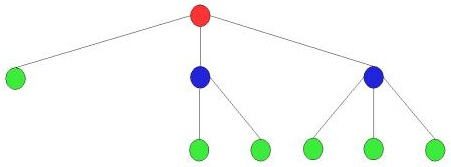
\includegraphics[width=0.5\columnwidth]{immagini/albero}
%	\caption[Albero]{Rappresentazione grafica di un albero}
%	%\label{fig:albero}
%\end{wrapfloat}

In questa implementazione ogni \emph{genitore}\index{genitore} può essere collegato al massimo a due \emph{figli}\index{figlio} pertanto l'albero prende il nome di \emph{\acl{bst}} {\small(\acs{bst})}, oppure \emph{albero binario} (figura~\ref{fig:bst}).
\`E possibile creare una struttura ``dal basso'', in cui ogni albero figlio contiene un campo puntatore al genitore.
\begin{figure}
	\centering
\begin{tikzpicture}[
	every node/.style = {
		circle,
	}
]
\tikzstyle{level 1}=[sibling distance = 25mm]
\tikzstyle{level 2}=[sibling distance = 13mm]
\tikzstyle{level 2}=[sibling distance = 10mm]

	\node [ball color = red] {}
		child {
			node [ball color=green] {}
		}
		child{
			node [ball color=blue] {}
				child{
					node [ball color=green] {}
				}
				child{
					node [ball color=green] {}
				}
		}
		child{
			node [ball color=blue] {}
				child{
					node [ball color=green] {}
				}
				child{
					node [ball color=green] {}
				}
				child{
					node [ball color=green] {}
				}
		};
\end{tikzpicture}
	\caption{Esempio di albero a più elementi.}
	\label{fig:+el-tree}
\end{figure}
Con questa modifica si possono ottenere alberi a più elementi come quello in figura~\ref{fig:+el-tree}.
%Tale modifica permette di avere un albero non più (soltanto) binario ma anche a più elementi.


%\begin{figure}
%	\centering
%\subfloat[Binary Search Tree][\emph{Binary Search Tree}\label{fig:bst1}]{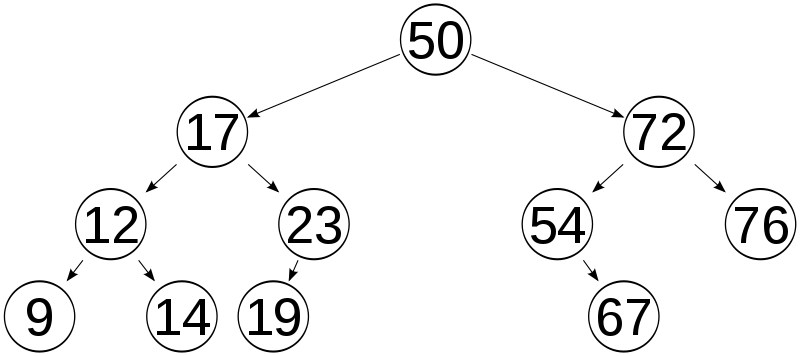
\includegraphics[width=\columnwidth]{immagini/bst_1}} \\
%\subfloat[BST con caratteri alfabetici][\emph{BST con caratteri alfabetici}\label{fig:bst_2}]{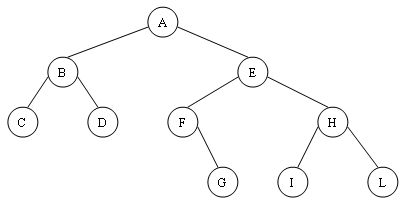
\includegraphics[width=0.45\columnwidth]{immagini/bst_2}} \quad
%\subfloat[Albero][\emph{Rappresentazione grafica di un albero}\label{fig:albero}]{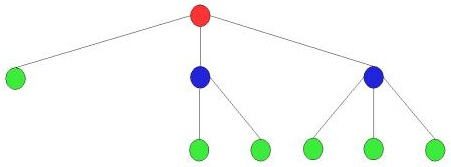
\includegraphics[width=0.45\columnwidth]{immagini/albero}}\\
%\subfloat[Lista concatenata bidirezionale][{\em Lista concatenata bidirezionale. I campi in blu sono puntatori.}\label{fig:blist}]{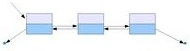
\includegraphics[width=0.45\columnwidth]{immagini/lista_bidirezionale}}\quad
%\subfloat[Coda][{\em Rappresentazione grafica di una coda.}\label{fig:coda}]{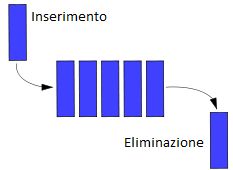
\includegraphics[width=0.45\columnwidth]{immagini/coda}}
%	\caption{Alcune strutture dati.}
%\end{figure}
%	\chapter{Domande e (alcune) risposte d'esame}
La maggior parte di questo e del prossimo capitolo è stata spudoratamente scopiazzata dalla mitica \href{http://it.wikipedia.org/wiki/Pagina_principale}{Viky Pedya} (sempre sia lodata), unica e sola fonte di salvezza degli studenti in crisi (e non). Mi sarebbe piaciuto attingere anche da siti più competenti come \href{http://nonciclopedia.wikia.com/wiki/Pagina_principale}{Nonciclopedia}, cui comunque rimando per \href{http://nonciclopedia.wikia.com/wiki/Motore_a_gatto_imburrato}{questo} articolo.


	\section{Domande d'Esame}
\begin{description}[]
	\item[Bernardinello's preface]
Questo documento ha lo scopo di aiutarvi nella preparazione dell'esame. Per superare l'esame è necessario saper rispondere correttamente alle domande che seguono (necessario ma non sufficiente).

Chi ha seguito il corso dovrebbe essere in grado di rispondere alla maggior parte delle domande. Per le domande più nozionistiche, vi è richiesto un piccolo sforzo di ricerca e documentazione. A questo scopo, sfruttate la biblioteca di ateneo; l'Internet è un'altra utile fonte di informazioni, ma va considerata inaffidabile.

Se non vi sentite in grado di rispondere a qualcuna delle domande, stabilite innanzitutto se la questione non è stata trattata a lezione in modo adeguato; in tal caso, segnalatemelo immediatamente.

L'elenco viene di tanto in tanto aggiornato. Tornate a consultarlo.
\newline
\newline
Luca Bernardinello

	

	\item[Fondamenti e Principi dell'Informatica:]\ 
	\begin{enumerate}
		\item
Chi era Alan Mathison Turing (vedi il paragrafo~\vref{subsec:turing})?
		\item
Che cos'è la Macchina di Turing? Che relazione ha con i calcolatori (vedi il paragrafo~\vref{subsec:mturing})?
		\item
Chi era John von Neumann? Descrivere la struttura generale di un calcolatore secondo von Neumann (vedi il paragrafo~\vref{sec:neu}).
		\item
Che cos'è un algoritmo? Dare una definizione il più possibile rigorosa.
	\end{enumerate}
	\item[Architettura dei Calcolatori e Sistemi Operativi:]\ 
	\begin{enumerate}[resume]
		\item
Descrivere la struttura di un calcolatore (vedi il paragrafo~\vref{sec:neu}).
		\item
 Che cos'è un \lstinline!bit!? Che cos'è un \lstinline!byte! (vedi il paragrafo~\vref{susec:bit})?
		\item
Che cos'è un \ac{os}? Quali sono le sue funzioni principali (vedi il paragrafo~\vref{subsec:sis})?
		\item
Come si interagisce con un \ac{os} (vedi il paragrafo~\vref{subsec:inter})?
	\end{enumerate}
	\item[Algoritmica e programmazione:]\ 
	\begin{enumerate}[resume]
		\item
Che cosa si intende per \emph{pseudocodice} (vedi il paragrafo ~\vref{sub:pseudo})?
		\item
Che cos'è un Linguaggio di Programmazione (vedi il paragrafo~\vref{subsec:programmazione})?
		\item
Che cosa si intende per Strutture Dati? Elencate e descrivete qualche struttura di dati dinamica (vedi il paragrafo~\vref{subsec:strutdat}).
		\item
Quali sono le Strutture di Controllo necessarie per esprimere un algoritmo (vedi il paragrafo~\vref{sec:ContStruc})?
		\item
Che cosa si intende per \emph{costo computazionale} di un algoritmo? Come si calcola?
		\item
L'algoritmo di ordinamento \emph{merge sort} ha un costo computazionale asintotico a $O(n\log_2 n)$. Che cosa vuol dire (vedi il paragrafo~\vref{subsec:eff})? (a proposito: che cos'è un algoritmo di ordinamento?)
		\item
Che differenza c'è fra costo computazionale di un algoritmo e costo computazionale di un problema?
		\item
Che cosa si intende per correttezza di un algoritmo? Come possiamo verificare se un algoritmo è corretto?
	\end{enumerate}
\end{description}

\newpage

\section{(Alcune) Risposte d'Esame}
	\subsection{Chi era Alan Mathison Turing?}
	\label{subsec:turing}

		\subsubsection{Introduzione}
\begin{wrapfloat}{figure}{i}{0pt}
	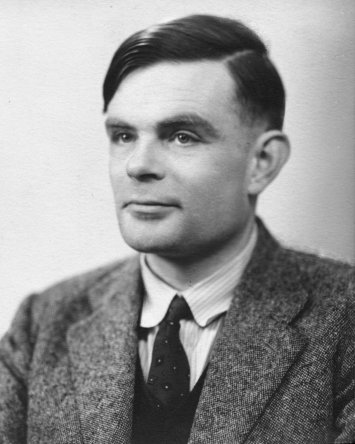
\includegraphics[width=0.6\columnwidth]{immagini/turing_photo}
	\caption[A. M. Turing]{Turing in una foto risalente al 29 Marzo 1951.}
	\label{fig:tur}
\end{wrapfloat}
Alan Mathison Turing (Londra, 23 giugno 1912 -- Wilmslow, 7 giugno 1954) è stato un matematico, logico e crittanalista britannico, considerato uno dei padri dell'informatica e uno dei più grandi matematici del Novecento. Introdusse la macchina ideale e fu anche uno dei più brillanti decrittatori che operavano in Inghilterra durante la seconda guerra mondiale per decifrare i messaggi scambiati da diplomatici e militari delle Potenze dell'Asse.

Omosessuale, morì suicida a soli 42 anni in seguito ad una persecuzione omofobica condotta nei suoi confronti. In suo onore la \ac{acm} ha creato nel 1966 il ""Turing Award'', massima riconoscenza nel campo dell'informatica, dei sistemi intelligenti e dell'intelligenza artificiale.

			\subsubsection{Biografia di Turing}
Turing\marginpar{Nascita} venne concepito in India, durante uno dei viaggi di suo padre, Julius Mathison Turing. Sia Julius che sua moglie, Ethel Sara Stoney, madre del futuro Alan Turing, decisero che il piccolo dovesse nascere sul suolo inglese. Tornarono quindi a Londra dove il 23 Giugno 1912 nacque Alan (figura~\vref{fig:tur}).

Già \marginpar{Infanzia e giovinezza} fin dalla più tenera età, Turing diede segno della genialità. Tuttavia, a causa della sua passione per le materie scientifiche divenne inviso ai professori del St. Michael, la sua prima scuola, i quali avevano sempre posto più enfasi sugli studi classici. Durante i primi anni di scuola ebbe quindi grosse difficoltà, ottenendo a stento il diploma. Poco appassionato al latino e alla religione, preferiva letture riguardanti la teoria della Relatività, i calcoli astronomici, la chimica o il gioco degli scacchi.

Nel\marginpar{Gli anni dell'Università} 1931 venne ammesso al King's College dell'Università di Cambridge dove approfondì i suoi studi sulla meccanica quantistica, la logica e la teoria della probabilità (dimostrò separatamente il \emph{Teorema Del Limite Centrale}, già dimostrato nel 1922 da Lindeberg). Nel 1934 si laureò con il massimo dei voti e nel 1936 vinse il Premio Smith (riconoscimento che veniva assegnato ai due migliori studenti ricercatori in Fisica e Matematica presso l'Università di Cambridge). Nello stesso anno si trasferì alla Princeton University dove studiò per due anni, ottenendo infine un Ph.D. In questi anni pubblicò l'articolo ""On computable Number, with an application to the Entscheidungsproblem'' dove descriveva, per la prima volta, quella che sarebbe poi stata definita come la \emph{macchina di Turing}.

Durante \marginpar{Il lavoro come crittografo} la seconda guerra mondiale, Turing mise le sue capacità matematiche al servizio del \emph{Department of Communications} inglese per decifrare i codici usati nelle comunicazioni tedesche. Con l'entrata in guerra dell'Inghilterra Turing fu ""arruolato'' nel gruppo di crittografi stabilitosi a Bletchley Park e con i suoi compagni lavorò stabilmente. Fu sul concetto di macchina di Turing che nel 1942 il matematico Max Newman progettò una macchina chiamata \emph{Colossus} (antesignana dei computer) che decifrava in modo veloce ed efficiente i codici tedeschi.

Al \marginpar{Il dopoguerra} termine della guerra Turing fu invitato al \ac{npl} a Londra per disegnare il modello di un computer. Il suo rapporto, che proponeva l'\ac{ace}, fu presentato nel marzo 1946 ma ebbe scarso successo a causa degli alti costi preventivati. Per l'anno accademico 1947/48 tornò a Cambridge e spostò i suoi interessi verso la neurologia e la fisiologia. Fu in questo periodo che iniziò ad esplorare la relazione tra i computer e la natura.

Nel \marginpar{Test di Turing} 1950 scrisse un articolo dal titolo ""Computing Machinery And Intelligence'' sulla rivista Mind in cui descriveva quello che sarebbe divenuto noto come il \emph{Test di Turing}. Su questo articolo si basa buona parte dei successivi studi sull'intelligenza artificiale.
L'anno seguente fu eletto Membro della Royal Society di Londra. Si trasferì all'Università di Manchester, dove lavorò alla realizzazione del \ac{madam}. Convinto che entro l'anno 2000 sarebbero state create delle macchine in grado di replicare la mente umana, lavorò alacremente creando algoritmi e programmi per il \ac{madam}, partecipò alla stesura del manuale operativo e ne divenne uno dei principali fruitori.

Nel \marginpar{Reclusione e morte} 1952 sviluppò un approccio matematico all'embriologia. Il 31 marzo dello stesso anno fu arrestato per omosessualità e condotto in giudizio, dove a sua difesa disse semplicemente che "<non scorgeva niente di male nelle sue azioni">. Secondo alcune fonti, Turing avrebbe denunciato per furto un suo amico ospite in casa sua ed ammesso la propria tendenza in risposta a delle domande pressanti della polizia. In quel periodo si dibatteva nel parlamento britannico l'abrogazione del reato di omosessualità e ciò probabilmente avrebbe indotto Turing ad un comportamento incauto. Fu sottoposto alla castrazione chimica, che lo rese impotente e gli causò lo sviluppo del seno; alcuni dei motivi che probabilmente lo condussero, di li a poco, al suicidio.
Nel 1954 Alan Turing morì ingerendo una mela avvelenata con cianuro di potassio, in tono col proprio carattere eccentrico e prendendo spunto dalla fiaba di Biancaneve da lui apprezzata fin da bambino. La madre sostenne che il figlio, con le dita sporche per qualche esperimento chimico, avesse ingerito per errore la dose fatale di veleno; ma il verdetto ufficiale parlò senza incertezze di suicidio:
\begin{quote}
"<Causa del decesso: cianuro di potassio autosomministrato in un momento di squilibrio mentale.">
\end{quote}


	\subsection{Che cos'è un \lstinline!bit!? Che cos'è un \lstinline!byte!?}
	\label{susec:bit}

In informatica, la parola \lstinline!bit! ha due significati molto diversi, a seconda del contesto in cui rispettivamente la si usa:
\begin{itemize}
	\item
\'E l'unità di misura dell'informazione (dall'inglese \emph{binary unit}), definita come la quantità minima di informazione che serve a discernere tra due possibili alternative equiprobabili;
	\item
\'E una \emph{cifra binaria}, (in inglese \emph{binary digit}) ovvero uno dei due simboli del sistema numerico binario, classicamente chiamati zero e uno (0 e 1).
\end{itemize}

Nella \marginpar{Il \lstinline!bit! come quantità d'informazione} prima accezione, un \lstinline!bit! rappresenta l'unità di misura della quantità d'informazione. Intuitivamente, equivale alla scelta tra due valori equiprobabili (sì/no, vero/falso\dots). Matematicamente, la quantità d'informazione in bit di un evento è l'opposto del logaritmo in base due della probabilità (sia essa $p$) di tale evento ($-\log_2 p$). La scelta del numero 2 come base del logaritmo è significativa nel caso elementare di scelta tra due alternative (informazione di un \lstinline!bit!), ma è possibile usare anche $e$ (numero di Nepero), usando dunque il logaritmo naturale ($-\ln p$). In tal caso l'unità di misura dell'informazione si dice \lstinline!Nat!.

Nel caso di due eventi equiprobabili, ognuno ha probabilità $1/2=0,5$. La loro quantità di informazione è, quindi, $-\log_2(1/2) = 1$ \lstinline!bit!.

Nella \marginpar{Il \lstinline!bit! come cifra binaria} seconda eccezione, il \lstinline!bit! rappresenta l'unità di definizione di uno stato logico. La rappresentazione logica del \lstinline!bit! è rappresentata dai soli valori \{$0$, $1$\}. Ai fini della programmazione è comune raggruppare sequenze di \lstinline!bit! in entità più vaste. Questi raggruppamenti contengono generalmente un numero di stringhe binarie pari ad una potenza binaria, pari cioè a $2^n$ con $n \in \mathbb{N} $. Il \marginpar{\emph{Il} byte} più noto è il \lstinline!byte! (chiamato anche \emph{ottetto}), corrispondente ad 8 \lstinline!bit!, che costituisce l'unità di misura più utilizzata in campo informatico.

Altri \marginpar{Altre unità di Misura} raggruppamenti di questo tipo sono i seguenti:
\begin{description}[]
	\item[Nibble:] 4 \lstinline!bit! (1/2 \lstinline!byte!);
	\item[Word:] di lunghezza variabile, corrisponde a 16, 32 o 64 \lstinline!bit!;
	\item[Double Word:] pari a 2 \lstinline!word! (\lstinline!DWORD! o \lstinline!LONGWORD!);
	\item[Quad Word:] pari a 4 \lstinline!word! (\lstinline!QWORD!);
	\item[Kibibyte:] 1024 \lstinline!byte!, indicato con \lstinline!KiB!;
	\item[Mebibyte:] 1024 \lstinline!kibibyte!, indicato con \lstinline!MiB!;
	\item[Gibibyte:] 1024 \lstinline!mebibyte!, indicato con \lstinline!GiB!;
	\item[Tebibyte:] 1024 \lstinline!gibibyte!, indicato con \lstinline!TiB!;
	\item[Pebibyte:] 1024 \lstinline!tebibyte!, indicato con \lstinline!PiB!;
	\item[Exbibyte:] 1024 \lstinline!pebibyte!, indicato con \lstinline!EiB!;
	\item[Zebibyte:] 1024 \lstinline!exbibyte!, indicato con \lstinline!ZiB!;
	\item[Yobibyte:] 1024 \lstinline!zebibyte!, indicato con \lstinline!YiB!.
\end{description}

	\subsection{Che cos'è un \acs{os}? Quali sono le sue funzioni principali?}
	\label{subsec:sis}

I'\ac{os} è un particolare software, installato su un sistema di elaborazione, senza il quale non è possibile l'utilizzo di altri software più specifici (in ultimo, del computer stesso). Esso quindi funge da ""base'' al quale si appoggiano gli altri software, che dovranno essere progettati in modo da essere riconosciuti e supportati da quel particolare sistema operativo. Per \marginpar{Definizione} \ac{os} s'intende dunque l'insieme dei componenti software che hanno il duplice scopo di gestire le risorse hardware e software del computer, ed interfacciare l'utente con l'hardware.

Secondo \marginpar{Funzioni Principali di un \ac{os}} una definizione più rigorosa, il sistema operativo è un insieme di subroutine e strutture dati responsabili di:
\begin{itemize}
	\item
Controllo e della gestione delle componenti hardware che costituiscono il computer (processi di Input/Output da/verso le periferiche collegate al sistema);
	\item
Esecuzione dei programmi che su di esso vengono eseguiti.
\end{itemize}
Se il sistema di elaborazione prevede la possibilità di memorizzazione aggiuntiva dei dati su memoria di massa, ha anche il compito di gestire l'archiviazione e l'accesso ai file. I programmi possono gestire l'archiviazione dei dati su memoria di massa (ottenendo strutture complesse, come un database), servendosi delle procedure messe a disposizione del sistema operativo. La componente dell'\ac{os} che si occupa di tutto ciò viene chiamata \emph{File System}.

Infine, se è prevista interazione con l'utente, viene solitamente utilizzata allo scopo un'interfaccia software (grafica o testuale) per accedere alle risorse hardware del sistema. Solitamente un \ac{os} installato su computer fornisce anche degli applicativi di base per svolgere elaborazioni di diverso tipo.

Al di là delle prestazioni massime offerte dall'hardware dell'elaboratore stesso, l'\ac{os} determina di fatto efficienza e buona parte delle prestazioni effettive di funzionamento dell'intero sistema ad esempio in termini di latenze di processamento, stabilità, interruzioni o crash di sistema.

Un \marginpar{Struttura} generico sistema operativo moderno si compone di alcune parti standard:
\begin{itemize}
	\item
\emph{Kernel}: gruppo di funzioni fondamentali, interconnesse fra loro e con l'hardware, che vengono eseguite con il privilegio massimo disponibile sulla macchina. Il kernel fornisce le funzionalità di base per tutte le altre componenti del sistema operativo, che assolvono le loro funzioni servendosi dei servizi che esso offre;
	\item
\emph{Gestore di File System}: si occupa di esaudire le richieste di accesso alle memorie di massa. Viene utilizzato ogni volta che si accede a un file su disco, e oltre a fornire i dati richiesti tiene traccia dei file aperti, dei permessi di accesso ai file. Inoltre si occupa anche e soprattutto dell'astrazione logica dei dati memorizzati sul computer (directory, ecc);
	\item
\emph{Sistema di Memoria Virtuale}: alloca la memoria richiesta dai programmi e dal sistema operativo stesso, salva sulla memoria di massa le zone di memoria temporaneamente non usate dai programmi e garantisce che le pagine swappate vengano riportate in memoria se richieste;
	\item
\emph{Scheduler}: che scandisce il tempo di esecuzione dei vari processi e assicura che ciascuno di essi venga eseguito per il tempo richiesto;
	\item
\emph{Spooler}: riceve dai programmi i dati da stampare e li stampa in successione, permettendo ai programmi di proseguire senza dover attendere la fine del processo di stampa;
	\item
\emph{Interfaccia utente \emph{(Shell)}}: permette agli esseri umani di interagire con la macchina.
\end{itemize}

	\subsection{Come si interagisce con un \acs{os}?}
	\label{subsec:inter}

Si distinguono due forme d'interazione con un \ac{os}:
\begin{enumerate}
	\item
Interazione gestuale;
	\item
Interazione verbale.
\end{enumerate}
Si parla d'\emph{interazione gestuale}\marginpar{Interazione Gestuale} quando l'utente impartisce comandi al sistema operativo compiendo gesti che sfruttano dispositivi fisici (mouse, tastiera\dots) ed elementi visivi (figurine, menu, finestre\dots). Questa è la forma oggi largamente più diffusa.

Si ha,\marginpar{Interazione Verbale} invece, \emph{interazione verbale} quando i comandi sono impartiti nel corso di un dialogo, sotto forma di parole o sigle. In questo caso l'interazione lascia una traccia su una console, che può occupare l'intero schermo oppure, ed è oggi il caso più frequente, una finestra sullo schermo. Le due forme di interazione possono quindi mescolarsi, e possiamo avere una sessione di interazione verbale nel contesto di un'interazione gestuale. Una \marginpar{Shell} sessione di interazione verbale è governata da un processo, quindi dall'esecuzione di un particolare programma, detto \emph{shell} (cioè ""guscio''). Nei sistemi operativi della famiglia Windows, questo guscio è denominato \emph{prompt dei comandi}. Nei sistemi UNIX, e nei suoi derivati, esistono numerose varianti di shell. Di norma, essa segnala il proprio stato di attesa di comando attraverso un invito (\emph{prompt}, appunto), cioè una particolare sequenza di caratteri visualizzata all'inizio della riga corrente nella console. La forma dell'invito varia da sistema a sistema, e può essere personalizzata da ogni singolo utente.


	\subsection{Che cosa si intende per \emph{pseudocodice}?}
	\label{sub:pseudo}
Per \emph{pseudocodice} (\emph{pseudolinguaggio} o \emph{linguaggio di progetto}) si intende un linguaggio di programmazione fittizio, non direttamente compilabile o interpretabile da un programma compilatore o interprete, il cui scopo è quello di rappresentare algoritmi. Lo pseudolinguaggio può essere utilizzato alternativamente al diagramma di flusso (\emph{flow cahrt}). Lo pseudolinguaggio dipende dal paradigma di programmazione scelto, mentre dovrebbe essere pressoché indipendente dal linguaggio di programmazione, purché quest'ultimo rispetti naturalmente il paradigma scelto.

	\subsection[Cosa si intende per Linguaggio di Programmazione?]{Che cos'è un Linguaggio di Programmazione?}
	\label{subsec:programmazione}

Un \marginpar{Definizione} \emph{linguaggio di programmazione} è un linguaggio formale, dotato di un lessico, di una sintassi e di una semantica ben definiti. È utilizzabile per il controllo del comportamento o la programmazione di una macchina formale attraverso la scrittura di un programma sotto forma di codice. \marginpar{Elementi ""obbligatori''} Tutti i linguaggi di programmazione possiedono:
\begin{itemize}
	\item
\emph{Variabile}: un dato o un insieme di dati, noti o ignoti, già memorizzati o da memorizzare; ad una variabile corrisponde sempre, da qualche parte, un certo numero (fisso o variabile) di locazioni di memoria che vengono allocate per contenere i dati stessi. Molti linguaggi attribuiscono alle variabili un tipo, con differenti proprietà;
	\item
\emph{Istruzione}: un comando o una regola descrittiva. Ogni volta che un'istruzione viene eseguita, lo stato interno del calcolatore cambia.
\end{itemize}
Alcuni \marginpar{Concetti frequenti} concetti sono poi presenti nella gran parte dei linguaggi:
\begin{itemize}
	\item
\emph{Espressione}: una combinazione di variabili e costanti, unite da operatori. Una espressione viene valutata per produrre un valore;
	\item
\emph{Strutture Dati}: meccanismi che permettono di organizzare e gestire dati complessi;
	\item
\emph{Strutture di Controllo}: permettono di governare il flusso d'esecuzione del programma, alterandolo in base al risultato o valutazione di una espressione;
	\item
\emph{Sottoprogramma} (funzione): un blocco di codice che può essere richiamato da qualsiasi altro punto del programma;
	\item
Funzionalità di input di dati da tastiera e visualizzazione dati in output (stampa a video).
\end{itemize}

	\subsection{Che cosa si intende per Strutture Dati? Elencate e descrivete qualche struttura di dati dinamica.}
	\label{subsec:strutdat}

Una \emph{struttura dati} è un'entità usata per organizzare un insieme di dati all'interno della memoria del computer. La scelta delle strutture dati è legata a quella degli algoritmi. Tale scelta, infatti, influisce inevitabilmente sull'efficienza degli algoritmi che la manipolano. La struttura dati è un metodo di organizzazione dei dati, quindi prescinde dai dati effettivamente contenuti.

I linguaggi di programmazione forniscono un insieme predefinito di tipi di dato elementari, e le strutture dati sono strumenti per costruire tipi di dati aggregati più complessi. Esse si differenziano soprattutto in base alle operazioni che si possono effettuare su di esse e alle prestazioni offerte.

		\subsubsection{Costruttori di Strutture Dati}
	
Un \marginpar{Array (o Vettore) [vedi il paragrafo~\vref{subsec:array}]} \emph{Array} è una struttura dati omogenea, che contiene un numero $n$ finito di elementi dello stesso tipo. Questi elementi sono individuati attraverso un indice numerico (da $0$ a $n-1$). La dimensione del vettore deve essere dichiarata al momento della sua creazione.

Un \marginpar{Record (o Struttura) [vedi il paragrafo~\vref{subsec:record}]}  \emph{Record} è una Struttura Dati che può essere eterogenea o omogenea. Nel primo caso contiene una combinazione di elementi che possono essere di diverso tipo. Questi sono detti \emph{campi}, e sono identificati da un nome.

		\subsubsection{Strutture Dati dinamiche}
Le Strutture Dati \emph{dinamiche} sono basate sull'uso di dati di tipo \emph{puntatore} e sull'allocazione dinamica della memoria. Lo spazio di memoria necessario per allocare i puntatori, e le operazioni necessarie alla loro manutenzione costituiscono il \emph{costo aggiuntivo} delle strutture dati dinamiche.

Una \marginpar{Lista Concatenata [vedi il paragrafo~\vref{subsec:liste}]}  \emph{Lista Concatenata} è un insieme di \emph{nodi} collegati linearmente. I nodi sono dei record che contengono un ""carico utile'' di dati, ed un puntatore all'elemento successivo della lista. L'ordine con cui sono collegati i nodi definisce un ordinamento tra di loro. Un nodo funge da testa della lista, e da questo è possibile accedere a tutti i nodi della lista. Conoscendo un nodo interno alla lista, è possibile accedere ai nodi successivi, ma non a quelli precedenti. Il costo di accesso ad un nodo della lista cresce con la dimensione della lista. Conoscendo il nodo precedente ad un nodo N, è possibile rimuovere N dalla lista, o inserire un elemento prima di lui, in un tempo costante.
	
Se \marginpar{Lista Bidirezionale}  la Lista è \emph{bidirezionale}, ogni nodo contiene un puntatore sia al precedente che al successivo. Usando la sintassi del linguaggio C, dato un nodo N il suo successore è \lstinline!N->succ!, e il suo precedente è \lstinline!N->prec!. Deve sempre essere vero che \lstinline!N->succ->prec == N!. Ogni nodo permette di accedere a tutti gli elementi della lista. Gli elementi ``strutturali'' di questa Struttura Dati, ovvero i due puntatori contenuti in ogni nodo, sono ridondanti

Un \marginpar{Alberi [vedi il paragrafo~\vref{subsec:albero}]} \emph{albero} è una rappresentazione dell'albero in teoria dei grafi. Ogni nodo contiene dei puntatori ad altri nodi che sono detti suoi \emph{figli}. Dato un nodo, è possibile accedere a tutti i suoi discendenti. Non deve essere possibile partire da un nodo, seguire i puntatori ai figli e ritornare al nodo di partenza. Inoltre ciascun nodo deve essere figlio di un solo \emph{padre}.

In alcune implementazioni, ogni nodo contiene un collegamento al suo padre. Tra i figli di un nodo esiste normalmente una relazione d'ordine, definita dall'ordine dei puntatori nel padre. In molte implementazioni, ogni nodo ha un numero fissato di figli, ad esempio due o tre. Si parla in questo caso di alberi \emph{binari} o \emph{ternari}. In altri casi, il numero di figli di un nodo è arbitrario.

Gli \marginpar{Binary Search Tree} alberi binari si prestano anche a rappresentare insiemi dotati di ordinamento: un nodo contiene un elemento dell'insieme da ordinare; tutti gli elementi collegati al primo figlio sono precedenti; quelli collegati al secondo sono successivi. Questi   alberi vengono anche definiti \emph{Binary Search Tree} (BST) ovvero alberi di ricerca binaria.
In questo modo, la ricerca di un elemento in un albero ordinato equilibrato richiede un tempo proporzionale al logaritmo del numero di elementi. L'inserimento di un elemento in un albero ordinato richiede di rispettare l'ordinamento precedentemente descritto.

		\subsubsection{Contenitori}
Le strutture dati sopra esposti possono essere utilizzate per realizzare alcuni tipi di \emph{contenitori} di utilizzo frequente, che possono forzare una particolare modalità di accesso ai dati.
	
Il \marginpar{Stack (o Pila) [vedi il paragrafo~\vref{subsec:stack}]} termine \emph{stack} (o pila) viene usato per riferirsi a strutture dati le cui modalità d'accesso seguono una politica LIFO (\emph{Last In First Out}), ovvero tale per cui i dati vengono estratti in ordine rigorosamente inverso rispetto a quello in cui sono stati inseriti. 
	Coda
Per \marginpar{Coda [paragrafo~\vref{subsec:coda}]} \emph{coda}, invece, s'intende una Struttura Dati di tipo FIFO, \emph{First In First Out} (il primo in ingresso è il primo ad uscire). Per implementare una coda viene utilizzato normalmente una Lista Concatenata. La Lista contiene due puntatori uno per la testa (il primo elemento della lista) e uno per la coda (ultimo elemento della Lista).
%	\chapter{Esempi di codici sorgenti}
\href{http://www.mc3.disco.unimib.it/lif/}{Sito} del Laboratorio d'Informatica I.
	\section{Esercitazione I}
Vai al \href{http://www.mc3.disco.unimib.it/lif/Dep/eslab1.pdf}{Testo dell'esercitazione}
		\lstinputlisting[caption=\emph{fahrchels.c}]{src/Es_1/fahrchels.c}
		\lstinputlisting[caption=\emph{valore\_assoluto.c}]{src/Es_1/valore_assoluto.c}

	\section{Esercitazione II}
Vai al \href{http://www.mc3.disco.unimib.it/lif/Dep/eslab2.pdf}{Testo dell'esercitazione}
		\lstinputlisting[caption={\em interi.c}]{src/Es_2/interi.c}
		\lstinputlisting[caption={\em pari\_dispari.c}]{src/Es_2/pari_dispari.c}

	\section{Esercitazione III}	
Vai al \href{http://www.mc3.disco.unimib.it/lif/Dep/eslab3.pdf}{Testo dell'esercitazione}
		\lstinputlisting[caption={\em euro\_dollaro.c}]{src/Es_3/euro_dollaro.c}
		\lstinputlisting[caption={\em primi.c}]{src/Es_3/primi.c}
		\lstinputlisting[caption={\em quadrati\_cubi.c}]{src/Es_3/quadrati_cubi.c}
		\lstinputlisting[caption={\em somma\_media\_max.c}]{src/Es_3/somma_media_max.c}

	\section{Esercitazione IV}
Vai al \href{http://www.mc3.disco.unimib.it/lif/Dep/eslab4.pdf}{Testo dell'esercitazione}
		\lstinputlisting[caption={\em esame.c}]{src/Es_4/esame.c}
		\lstinputlisting[caption={\em e\_nepero.c}]{src/Es_4/e_nepero.c}
		\lstinputlisting[caption={\em funzioni.c}]{src/Es_4/funzioni.c}
		\lstinputlisting[caption={\em ordinamento.c}]{src/Es_4/ordinamento.c}	

	\section{Esercitazione V}
Vai al \href{http://www.mc3.disco.unimib.it/lif/Dep/eslab5.pdf}{Testo dell'esercitazione}
		\lstinputlisting[caption={\em dadi.c}]{src/Es_5/dadi.c}
		\lstinputlisting[caption={\em distribuzione.c}]{src/Es_5/distribuzione.c}
		\lstinputlisting[caption={\em schemaop\_complessi.c}]{src/Es_5/schemaop_complessi.c}

	\section{Esercitazione VI}
Vai al \href{http://www.mc3.disco.unimib.it/lif/Dep/eslab6.pdf}{Testo dell'esercitazione}
		\lstinputlisting[caption={\em calcolo\_postfissa.c}]{src/Es_6/calcolo_postfissa.c}
		\lstinputlisting[caption={\em infix\_postfix.c}]{src/Es_6/infix_postfix.c}
		\lstinputlisting[caption={\em radice.c}]{src/Es_6/radice.c}

	\section{Esercitazione VII}
Vai al \href{http://www.mc3.disco.unimib.it/lif/Dep/eslab7.pdf}{Testo dell'esercitazione}	
		\lstinputlisting[caption={\em binario\_decimale.c}]{src/Es_7/binario_decimale.c}

		\appendix
	\chapter{Appunti vari}
	\section{Stack}
	\label{sec:vari:stack}
Come già detto, si può usare un vettore come \emph{stack} (pila), dichiarandolo abbastanza lungo e supponendo che le operazioni aritmetiche stiano all'interno della lunghezza del vettore.
Ci si può servire di una variabile intera che punti alla prima posizione libera del vettore.
Per ogni operazione \emph{push}, si copia il nuovo valore nella posizione dell'indice e s'aggiorna il valore di quest'ultimo.
Nel caso dell'operazione \emph{pop} si dovrà leggere il valore della variabile due caselle a sinistra dell'indice e spostare quest'ultimo di una posizione a sinistra.

	\section[Editor di testo \textsf{vi(m)}]{Editor di testo vi(m)}

Sull'editor di testo \textsf{Vi} o, nella versione corrente, \textsf{Vim} cioè \emph{Vi Improved}, ci sono due modalità:
\begin{itemize}
	\item Modo inserimento;
	\item Modo comando.
\end{itemize}
Quando il programma viene avviato è in \emph{modalità comando}, in attesa di riceverne uno dall'utente.
Premendo il tasto \key{I}, l'editor passa in \emph{modalità inserimento}: è possibile scrivere alla sinistra del cursore e modificare il documento.
Premendo il tasto \key{A} in modalità comando, invece, si comincia a scrivere a destra del cursore mentre per uscire dalla modalità inserimento si usa \key{Esc}.
Il tasto \key{O}, in modalità comando, apre una nuova riga sotto la posizione del cursore mentre la combinazione \key{Maiusc + O} ne apre una sopra la posizione del cursore.


Quando il cursore si sposta su una parentesi aperta, il programma evidenzia la parentesi chiusa corrispondente.
Per cancellare un carattere in modo comando basta spostare il cursore sopra il carattere da cancellare e premere il tasto \key{X}; per cancellare l'intera riga, ci si sposta all'inizio della riga e si preme il tasto \key{D} due volte.


In modalità comando, alla pressione del tasto \key{:}, ossia \key{Maiusc + .}, il programma aspetta si dei comandi.
Ad esempio, per salvare le modifiche al file si usa \lstinline!:w! (che sta per \emph{write}); per uscire e ritornare all'ambiente \emph{shell} da cui il programma è stato lanciato si usa \lstinline!:q! (ossia \emph{quit}).
%A questo punto, volendo, è possibile tornare a lavorare sul file salvato.
Il comando \lstinline!:w! può salvare il documento in un file diverso da quello su cui si sta lavorando tramite la sintassi 
\begin{lstlisting}
:w £!\MyComment{nome del file}!£
\end{lstlisting}
mentre la combinazione \lstinline!:wq! salva ed esce.

	\section{Debugger}
Il \emph{debugger}\index{debugger} è un programma progettato per l'analisi e l'eliminazione dei bug (vedi il paragrafo~\ref{sec:bug}) presenti in altri software.
Assieme al compilatore è fra i più importanti strumenti di sviluppo a disposizione di un programmatore.
Il compito principale del debugger è di mostrare il frammento di codice che genera il problema (tipicamente un \emph{crash}).

	\section{Bug}
	\label{sec:bug}
Nell'informatica il termine \emph{bug}\index{bug} (o baco) identifica un errore nella scrittura di un programma software.
Meno comunemente, può indicare un difetto di progettazione in un componente hardware.
Un bug di un programma è un errore che porta al malfunzionamento dello stesso.
La causa del maggior numero di bug è spesso il codice sorgente scritto da un programmatore, ma può anche accadere che venga prodotto dal compilatore.


\backmatter
	\listoffigures
%	\addcontentsline{toc}{chapter}{\tocEntry{\listfigurename}}
	\addcontentsline{toc}{chapter}{\listfigurename}

	\listoftables
%	\addcontentsline{toc}{chapter}{\tocEntry{\listtablename}}
	\addcontentsline{toc}{chapter}{\listtablename}

	\lstlistoflistings
%	\addcontentsline{toc}{chapter}{\tocEntry{\lstlistlistingname}}
	\addcontentsline{toc}{chapter}{\lstlistlistingname}

	\chapter{Elenco degli acronimi}
\begin{acronym}[MADAM]
	\acro{cpu}[CPU]{Central Process Unit}
{\small\par\noindent L'\emph{Unità Centrale d'Elaborazione} è la parte del computer che si occupa di trasformare e manipolare i dati.}
	\acro{ram}[RAM]{Random Access Memory}
{\small\par\noindent La \emph{Memoria di Lavoro} conserva i dati durante l'esecuzione di un programma o la loro elaborazione.}
	\acro{io}[I/O]{Input/Output}
{\small\par\noindent Le unità di \emph{Ingresso/Uscita} consentono di immettere/acquisire i dati dal calcolatore}
	\acro{os}[OS]{Operating System}
	\acro{acm}[ACM]{Association for Computing Machinery}
	\acro{npl}[NPL]{National Physical Laboratory}
	\acro{ace}[ACE]{Automatic Computing Engine}
	\acro{madam}[MADAM]{Manchester Automatical Digital Machine}
\end{acronym}

%\clearpage
%\phantomsection
\addcontentsline{toc}{section}{\indexname}
\printindex


	\nocite{*}
	\printbibliography
%	\bibliographystyle{plainnat}
%	\bibliography{bibliografia}
%	\addcontentsline{toc}{chapter}{\tocEntry{\bibname}}
	\addcontentsline{toc}{chapter}{\bibname}
\end{document}